\documentclass[11pt,a4paper]{article}
\usepackage[T1]{fontenc}
\usepackage[utf8]{inputenc}
\usepackage{lmodern}
\usepackage[margin=25mm,headheight=15pt]{geometry}
\usepackage{amsmath,amssymb,amsthm,mathtools}
\usepackage{booktabs,tabularx,array,longtable}
\usepackage{enumitem,microtype,xcolor,fancyhdr}
\usepackage{tikz}
\usetikzlibrary{positioning,arrows.meta,calc}
\usepackage[hyphens]{url}
\usepackage{hyperref}
\definecolor{inkblue}{RGB}{27,48,72}
\definecolor{aworld}{RGB}{160,60,40}
\definecolor{bworld}{RGB}{30,90,140}
\definecolor{wild}{RGB}{40,110,70}
\hypersetup{colorlinks=true,linkcolor=inkblue,citecolor=inkblue,urlcolor=inkblue,
 pdftitle={The two-world search for Euler's constant},pdfauthor={KEIO}}
\newcommand{\Q}{\mathbb Q}
\newcommand{\R}{\mathbb R}
\newcommand{\Z}{\mathbb Z}
\newcommand{\C}{\mathbb C}
\newcommand{\Qbar}{\overline{\mathbb Q}}
\newcommand{\Ein}{\operatorname{Ein}}
\newcommand{\EE}{\mathbf E}
\newcommand{\GG}{\mathbf G}
\newcommand{\DD}{\mathbf D}
\newcommand{\MM}{\mathbf M}
\newcommand{\Sring}{\mathbf S}
\newcommand{\Vring}{\mathbf V}
\newcommand{\Dhat}{\widehat D}
\newcommand{\Fld}{\mathbb F}
\newcommand{\Th}{\mathcal K}
\newcommand{\Tth}{\mathcal T}
\newcommand{\shear}{\mathfrak s}
\newcommand{\Tz}{T_0}
\newcommand{\Pc}{\mathcal P}
\newcommand{\Aff}{\mathcal A}
\DeclareMathOperator{\trdeg}{trdeg}
\DeclareMathOperator{\den}{den}
\DeclareMathOperator{\house}{house}
\DeclareMathOperator{\Bsum}{\mathcal S}
\DeclareMathOperator{\Ht}{H}
\DeclareMathOperator{\spn}{span}
\DeclareMathOperator{\Nm}{N}
\DeclareMathOperator{\Res}{Res}
\newtheorem{theorem}{Theorem}[section]
\newtheorem{proposition}[theorem]{Proposition}
\newtheorem{lemma}[theorem]{Lemma}
\newtheorem{corollary}[theorem]{Corollary}
\theoremstyle{definition}
\newtheorem{definition}[theorem]{Definition}
\newtheorem{problem}[theorem]{Problem}
\newtheorem{example}[theorem]{Example}
\newtheorem{specification}[theorem]{Specification}
\newtheorem{question}[theorem]{Question}
\theoremstyle{remark}
\newtheorem{remark}[theorem]{Remark}
\numberwithin{equation}{section}
\setlist[enumerate]{topsep=4pt}
\setlength{\emergencystretch}{3em}
\setlength{\parskip}{2pt}
\allowdisplaybreaks[2]
\pagestyle{fancy}
\fancyhf{}
\fancyhead[L]{\small KEIO}
\fancyhead[R]{\small The two-world search for Euler's constant}
\fancyfoot[C]{\thepage}
\renewcommand{\headrulewidth}{0.3pt}
\newenvironment{partsummary}[1]{\begin{quotation}\small\noindent\textbf{Summary of Part~#1.}\ }{\end{quotation}}

\title{\bfseries The Two-World Search for Euler's Constant\\[6pt]
\large Shear invariance, collision worlds, forgeries, and the map of possible worlds}
\author{KEIO\thanks{Prepared in a working session with Claude (Anthropic), 10--11 September 2026,
as a companion to the cumulative manuscript \cite{M} and its companions \cite{K001,K002}.
The five parts were written in sequence, each derived for this work and then compared with
the literature; coincidences with published results are indicated where they occur. Every
number was recomputed by the archived scripts (Appendix~\ref{app:archive}). No claim of
external review is made; each part was checked by an internal referee pass whose findings
were incorporated.}}
\date{11 September 2026}

\begin{document}
\maketitle

\begin{abstract}
Let $\gamma$ be Euler's constant, $\Ein(z)=\sum_{n\ge1}(-1)^{n-1}z^n/(n\,n!)$, and
$\delta=eE_1(1)$ the Euler--Gompertz constant, so that $\Ein(1)=\gamma+\delta/e$. We
study the alternative $\mathrm A$: $\gamma\in\Qbar$ against $\mathrm B$: $\gamma\notin\Qbar$
by building inside each world and asking what ordinary mathematics can reject. The
outcome is a structure theorem rather than a decision. Every unconditional arithmetic
theorem in which $\gamma$ occurs that we could identify is invariant under a
\emph{framing shear} $\gamma\mapsto c$, $E_1(\lambda)\mapsto E_1(\lambda)+\gamma-c$,
$\delta\mapsto\delta+e(\gamma-c)$, and the theory generated by shear-invariant statements
and finitely many numerical enclosures has models in which the constant standing for
$\gamma$ is algebraic and models in which it is transcendental; more generally no
shear-invariant theorem places $\gamma$ inside or outside any class that is dense with
dense complement (algebraic numbers, $E$-, $G$-, $D$-values, periods, logarithms). On the
level of functions the shear is the twist $\Gamma\mapsto\Gamma(s)e^{\tau(1-s)}$, which
preserves every connection identity and moves the Euler constant to $\gamma+\tau$; on
linear forms it forces the tie $|b-ec|\le2\eta/\ell$, so shear-invariant families of integer
forms in $1,\gamma,\delta$ have exponent at most $1$, generically $\tfrac12$, which
Rivoal's forms realise ($b_n/c_n-e=1.4\cdot10^{-255}$ at $n=39$). The sharpest consequences
of $\mathrm A$ are derived (the collision $\delta\in(\EE\cap\DD)\setminus\Qbar$; the floor
$|a+b\gamma+c\delta|\ge H^{-(d3^d-1)-\varepsilon}$; $\mu(\delta)=2$ if $\gamma\in\Q$; the
reduction to ``is $\delta$ an $E$-value''; the collision spectrum of the polyexponential
tower) and compared with what is provable; a ledger of twelve $\mathrm A$-constructions
shows that every one expected to be false is a membership statement whose rejection is a
known conjecture at one element. Built for their own sake, the worlds acquire shadow
systems of honest $E$-values, phantom Galois conjugates, a Galois norm, certificate loci
dual to the $\mathrm A$-world's Beukers theory, a gallery of forgeries (explicit members
of ten worlds agreeing with $\gamma$ to $30$ and $100$ digits at the uniform price
$\Ht\approx10^{p/(m+1)}$), and a map of the possible worlds on which the expected truth is
the wild region where no integer-relation search can succeed. Certified lattice
computations accompany every finite claim. Nothing here proves the irrationality or
transcendence of $\gamma$ or $\delta$; what is proved is why the available tools cannot,
and what the first tool that could would have to look like.
\end{abstract}

\tableofcontents

\section{Introduction}\label{sec:introduction}

\subsection{The question and the programme}

Whether Euler's constant $\gamma=\lim_n(H_n-\log n)$ is irrational, let alone
transcendental, is open. The cumulative manuscript \cite{M} and its companions
\cite{K001,K002} developed the arithmetic of $\gamma$ through the exponential integral:
the $E$-function $\Ein(z)$ satisfies the connection formula
$\Ein(z)=\gamma+\log z+E_1(z)$, its value at $1$ is $\gamma+\delta/e$ with $\delta$ the
Euler--Gompertz constant, and the pair $(\gamma,\delta)$ sits at the meeting point of the
two rings of Fischler and Rivoal: the ring $\EE$ of values of $E$-functions at algebraic
points and the ring $\DD$ of Borel sums of arithmetic Gevrey series.

This paper records a programme proposed in the working session that produced it. Instead
of attacking $\gamma$ directly, one splits mathematics into two worlds,
\[
 \mathrm A:\ \gamma\in\Qbar\qquad\text{and}\qquad\mathrm B:\ \gamma\notin\Qbar ,
\]
builds inside each---derives consequences, constructs objects, computes---and asks
whether the real world $\mathrm C$ (mathematics as it stands) rejects anything so built.
Fermat's Last Theorem is the model: the consequence ``a Frey curve exists'' was rejected by
modularity, a theorem about objects of a different kind. The question is whether $\gamma$
admits an analogue of the Frey curve. The programme was run in five stages, and the five
parts of this paper are those stages, lightly edited and cross-referenced but otherwise as
written, so that the reader can see what was tried, in what order, and where each attempt
stopped.

\subsection{What was found}

The answer to the programme's question is structural, and it is the main result.

\emph{The shear.} Every unconditional arithmetic theorem in which $\gamma$ occurs that we
could identify reaches $\gamma$ only through connection formulas of the type
$\Ein(\lambda)=\gamma+\log\lambda+E_1(\lambda)$, and is therefore invariant under the
\emph{framing shear} $\gamma\mapsto c$, $E_1(\lambda)\mapsto E_1(\lambda)+\gamma-c$,
$\delta\mapsto\delta+e(\gamma-c)$ (Part~I, Section~\ref{I:sec:shear}). The theory
$\Th(\Fld;\mathcal C)$ generated by shear-invariant statements together with finitely many
numerical enclosures has models in which the constant standing for $\gamma$ is algebraic
and models in which it is transcendental (Theorem~\ref{I:thm:two-models}); no
shear-invariant theorem places $\gamma$, $\delta$ or $E_1(\lambda)$ inside or outside any
class that is dense with dense complement (Theorem~\ref{III:thm:density},
Corollary~\ref{III:cor:invisible}); and in every terminating pair of construction and
rejection at least one half must use an analytic definition of the constant
(Corollary~\ref{III:cor:filter}). At the level of functions the shear is the twist
$\Gamma_\tau(s)=\Gamma(s)e^{\tau(1-s)}$, which preserves every connection identity, moves
the Euler constant to $\gamma+\tau$, acts on the polyexponential tower as the rescaling
$\lambda\mapsto\lambda e^\tau$, and breaks only the normalisations of the classical
Gamma identities (Proposition~\ref{IV:prop:twist}, Remark~\ref{IV:rem:bohr}); it extends to
the incomplete Gamma function and to the mixed values of Fischler--Rivoal, fixing the
$E$-side and moving the $D$-side (Propositions~\ref{V:prop:incgamma}
and~\ref{V:prop:mixed}). On the period matrix of Fres\'an--Jossen it is a $\C$-linear
change of de Rham basis fixing the period $\Ein(1)$ of the cycle $\sigma_1+\sigma_2$
(Remark~\ref{IV:rem:FJ}).

\emph{The quantitative shadow of the shear.} A bound $|a+b\Gamma+c\Delta|<\eta$ proved
shear-invariantly forces $|b-ec|\le2\eta/\ell$ (Theorem~\ref{III:thm:tie}); hence
shear-invariant families of integer forms in $1,\gamma,\delta$ have exponent at most $1$,
generically $\tfrac12$, and can never meet Nesterenko's threshold
(Corollary~\ref{III:cor:ceiling}). Rivoal's forms are verified to be tied, $b_n/c_n\to e$
(Proposition~\ref{III:prop:rivoal-tie}), lattice-optimal shear-invariant forms sit at
exponent $0.50$--$0.54$, and the $D$-side Stieltjes forms are untied but grow
(Proposition~\ref{III:prop:stieltjes}). The first Diophantine construction that could
matter is thereby specified: integer forms smaller than their own tie defect, equivalently
engine ratios $-(a_n+c_ne\Ein(1))/(b_n-ec_n)$ converging to $\gamma$ with a proof that uses
a bridge (Specification~\ref{III:spec}).

\emph{What $\mathrm A$ implies.} Under $\mathrm A$, $\delta\in(\EE\cap\DD)\setminus\Qbar$
(Proposition~\ref{I:prop:A-basic}); integer forms obey the floor
$|a+b\gamma+c\delta|\ge c_\varepsilon H^{-(d3^d-1)-\varepsilon}$ (Theorem~\ref{I:thm:floor});
$\mu(\delta)=2$ if $\gamma\in\Q$ (Proposition~\ref{I:prop:rational}); the whole question
reduces to ``is $\delta$ an $E$-value'' (Theorem~\ref{I:thm:E-reduction}); the
polyexponential tower has an explicit collision spectrum, $\omega_{\lambda,r}\in\EE$ iff
$P_r(\lambda)=[t^r]\bigl(\Gamma(1-t)\lambda^t\bigr)\in\EE$
(Theorem~\ref{II:thm:spectrum}), and $\mathrm A$ forces only the collision at $(1,1)$
(Corollary~\ref{II:cor:forced}); the $\mathrm A$-world proves, by Beukers' theorem, that
$\{1,e^\lambda,\Ein(\lambda)-\gamma\}_{\lambda\in\Lambda}$ is linearly independent for
every finite $\Lambda$ (Theorem~\ref{IV:thm:Aworld}), a sentence $\mathrm C$ does not at
present prove. The ledger of Part~III (Table~\ref{III:tab:ledger},
Proposition~\ref{III:prop:pattern}) shows the pattern: every $\mathrm A$-construction
expected to be false is a membership, dependence or splitting statement whose rejection
is a known conjecture---$\EE\cap\DD=\Qbar$, fullness of the period realisation,
$\gamma\notin\EE$---evaluated at one element; every Diophantine construction is expected
to be true or is a finite certificate. A linear hierarchy
$\mathrm B\Leftarrow\mathrm X(\Qbar+\Qbar e)\Leftarrow\mathrm X(W)\Leftarrow\mathrm X(\EE)$
grades the distance between what is known and what is wanted
(Theorem~\ref{III:thm:hierarchy}).

\emph{The worlds for their own sake.} For every algebraic $c$ the \emph{shadow system}
$(c,\delta_c=e(\Ein(1)-c),E_1(\lambda)_c)$ satisfies all connection identities and consists
of $E$-values, $\delta_c=\sum_n(H_n-c)/n!$ (Proposition~\ref{IV:prop:shadowE}); the
$\mathrm A$-world has $d-1$ phantom Galois conjugates and a Galois norm
$P_\gamma(\Ein(1))=\prod_\sigma E_1(1)^{(\sigma)}$ (Proposition~\ref{IV:prop:galois}). Every
certificate is a camouflage read backwards: the lattice vector certifying ``no relation of
degree $\le12$ below height $\approx10^{p/13}$'' is the minimal polynomial of an algebraic
number within $10^{-p}$ of $\gamma$ (Proposition~\ref{IV:prop:duality}), and the same holds
on every certificate locus, giving the gallery of forgeries of Part~V
(Proposition~\ref{V:prop:gallery}) with the uniform price $\Ht\approx10^{p/(m+1)}$. The
$\mathrm A$-world's theorems dualise into \emph{certificate loci} of the $\mathrm B$-world
(Proposition~\ref{IV:prop:dual}), searched in Proposition~\ref{IV:prop:zoo}; the expected
truth is the \emph{wild world}, where no integer-relation search can succeed
(Proposition~\ref{IV:prop:wild}). The map of possible worlds (Figure~\ref{IV:fig:map})
records which theorem certifies against, and which conjecture is expected to remove, each
region.

\emph{The verdict.} No contradiction was found in either world, and by
Lemma~\ref{III:lem:bookkeeping} none could be found without proving $\mathrm B$. What the
programme produced is a classification of the tools by their relation to the shear, three
quantified barriers (Section~\ref{III:sec:outcome}), and three sharpened targets: forms
below their tie defect; the point conjecture $\mathrm B_\delta$:
$\delta\in\EE\Rightarrow\delta\in\Qbar$ (Definition~\ref{II:def:dichotomy}); and fullness of
the period realisation for the Euler--Mascheroni motive.

\subsection{Conventions}

\textbf{Status conventions.} As in \cite{M}: \emph{auxiliary theorem} (proved here with
displayed hypotheses), \emph{published input} (attributed), \emph{preprint input}
(attributed to an unpublished but publicly available source and used only in explicitly
labelled statements), \emph{finite certificate} (a computation with exact
re-verification), \emph{conditional implication}, \emph{open target}. Nothing in this
paper proves the irrationality or transcendence of $\gamma$ or $\delta$. Where a statement
coincides with a published result this is said explicitly; the framework of Fischler and
Rivoal \cite{FR2016,FR2018,FRmixed}, Beukers' lifting theorem \cite{Beukers}, and the
exponential motives of Fres\'an and Jossen \cite{FJ} are used throughout.

\textbf{Notation.} We write $H_n=\sum_{k\le n}1/k$ and $\Ein_r(z)=\sum_{n\ge1}(-1)^{n-1}z^n/(n^rn!)$,
with $\Ein=\Ein_1$; $E_1(z)=\int_z^\infty e^{-t}\,dt/t$ is the exponential integral and
$\delta=eE_1(1)=\int_0^\infty e^{-t}(1+t)^{-1}\,dt$ the Euler--Gompertz constant. The
connection formula is $\Ein(z)=\gamma+\log z+E_1(z)$ (principal logarithm), with the
instance $\Ein(1)=\gamma+\delta/e$. The rings $\EE$, $\GG$, $\DD$, $\Sring$ and
$\Vring=\Sring\cdot\EE$ are defined in Part~II, Section~\ref{II:sec:setup}; $\Ht$ is the
naive height and $\mu$ the irrationality exponent. Each part opens with its original
summary and closes with its computations; the scripts are collected in
Appendix~\ref{app:archive}. Cross-references between parts are internal.

\textbf{Reading order.} Part~I is the framework and can be read alone. Part~II re-runs the
search on the ring dichotomy and is independent of Part~III. Part~III is the ledger and
uses Parts~I--II. Parts~IV and~V build without aiming at termination and use everything
before them; a reader interested only in the shear as a twist of the Gamma function can
read Part~IV, Section~\ref{IV:sec:twist}, and Part~V, Section~\ref{V:sec:twist}, after
Part~I, Section~\ref{I:sec:shear}.

\part{The framework: symmetry of finite observations, the framing shear, and the two models}
\begin{partsummary}{I}
The cumulative manuscript names the two arithmetic alternatives for Euler's constant
$\mathrm A$: $\gamma\in\Qbar$ and $\mathrm B$: $\gamma\notin\Qbar$, and asks whether
consequences derived under $\mathrm A$ and under $\mathrm B$ must eventually collide
with an established fact. This note runs that search as far as it can currently go and
records the outcome. No collision is obtained. Instead we observe that every
unconditional arithmetic theorem in which $\gamma$ occurs that we could identify is
invariant under a \emph{framing shear} $\gamma\mapsto c$,
$E_1(\lambda)\mapsto E_1(\lambda)+\gamma-c$, which fixes all $E$-values, exponentials,
logarithms and periods, and we prove that the theory generated by shear-invariant
statements together with finitely many numerical enclosures has models in which the
constant standing for $\gamma$ is interpreted by an algebraic number and models in which
it is interpreted by a transcendental number, so the search cannot terminate on that
theory. We then derive the sharpest consequences of $\mathrm A$ that we
can state with published inputs---$\delta\in\EE\cap\DD$ with $\delta\notin\Qbar$, an
explicit lower bound $|a+b\gamma+c\delta|\ge H^{-(d3^d-1)-\varepsilon}$ for integer
linear forms when $\gamma$ has degree $d$, and $\mu(\delta)=2$ when $\gamma$ is rational---and
compare them with what the established world can supply (Rivoal-type explicit forms are
guaranteed exponent $1/2-o(1)$ and deliver about $1/4$; continued-fraction data give
$2.000$). Finally we show that
the whole search reduces to the single question ``is $\delta$ (equivalently $\gamma$, or
$E_1(1)$) a value of an $E$-function at an algebraic point?'': a positive answer makes the
algebraicity of $\gamma$ a terminating computation (Adamczewski--Rivoal) once an explicit
representation is given, and a
negative answer proves transcendence. Neither answer is presently available, and the only
known certificates of non-membership in $\EE$ are Diophantine. Finite certificates are
pushed further with exact LLL data (no relation of degree $\le30$ and height
$<10^{73}$), and a degree-$12$ algebraic integer agreeing with $\gamma$ to $30$ decimals with
full local counts at $2$ and $3$ is exhibited to show why such certificates cannot close the
question.
\end{partsummary}


\section{The proposal and the outcome}\label{I:sec:scope}

Throughout,
\begin{equation}\label{I:eq:defs}
\begin{gathered}
 \gamma=\lim_{n\to\infty}(H_n-\log n),\qquad
 \Ein(z)=\sum_{n\ge1}\frac{(-1)^{n-1}z^n}{n\,n!},\\
 E_1(x)=\int_x^\infty\frac{e^{-t}}t\,dt,\qquad
 \delta=\int_0^\infty\frac{e^{-t}}{1+t}\,dt=eE_1(1),
\end{gathered}
\end{equation}
and on the positive real axis $\Ein(x)=\gamma+\log x+E_1(x)$, so that
$\eta:=\Ein(1)=\gamma+\delta/e$. Let $\Tth$ be the body of established mathematics
(any fixed consistent effectively axiomatized theory containing the definitions above will
do), let $\mathrm A$ be the sentence $\gamma\in\Qbar$ and $\mathrm B=\neg\mathrm A$.
The proposal is: derive in $\Tth+\mathrm A$, derive in $\Tth+\mathrm B$, and wait for a
contradiction in $\Tth$.

The bookkeeping is recorded in the cumulative manuscript
\cite[Part~VI]{M}: $\Tth+\mathrm A\vdash\bot$ if and only if $\Tth\vdash\mathrm B$, and
$\Tth+\mathrm B\vdash\bot$ if and only if $\Tth\vdash\mathrm A$, so the parallel search
terminates exactly when $\Tth$ decides $\mathrm A$. The practical question is therefore
not whether the search terminates in principle but on which \emph{sub-theory}
$\Th\subset\Tth$ it can be run, namely on the theorems actually available. The outcome
of this note is the following.

\begin{enumerate}[leftmargin=*]
\item \textbf{The available sub-theory does not decide $\mathrm A$.} Section~\ref{I:sec:shear}
proves that the theory $\Th$ generated by (i) all true statements about any field of
constants $\Fld$---in particular the engine field $\Fld_0$ generated by all $E$-values and
all classical periods, hence by all exponentials, logarithms, $G$-values, Bessel and Gamma
values---, (ii) the connection identities
$E_1(\lambda)=\Ein(\lambda)-\gamma-\log\lambda$ and $\delta=eE_1(1)$, and (iii) finitely
many true numerical enclosures, has a model in which the constant standing for $\gamma$
is algebraic and a model in which it is transcendental (Theorem~\ref{I:thm:two-models}). Every unconditional
arithmetic theorem about $\gamma$ known to us is provable in $\Th$
(Remark~\ref{I:rem:inventory}), because each of them reaches $\gamma$ only through the
connection identities. The manuscript's Stokes-framing barrier
\cite[\S``The Stokes-framing barrier'']{K002} is the differential-Galois face of the same
shear.
\item \textbf{The $\mathrm A$-world makes sharp, testable-looking predictions, and all of
them survive every test.} Section~\ref{I:sec:A} derives them:
$\delta\in\EE\cap\DD$ and $\delta\notin\Qbar$ (Proposition~\ref{I:prop:A-basic});
a lower bound for integer linear forms in $1,\gamma,\delta$ with explicit exponent
$d3^d-1$ (Theorem~\ref{I:thm:floor}); $\mu(\delta)=2$ if $\gamma\in\Q$
(Proposition~\ref{I:prop:rational}). Section~\ref{I:sec:computations} compares them with the
best explicit constructions: Rivoal-type linear forms are guaranteed exponent
$1/2-o(1)$ and deliver about $1/4$ (Table~\ref{I:tab:rivoal}), continued-fraction
convergents of $\delta$ have exponent $2.000$
(Table~\ref{I:tab:cf}).
\item \textbf{The search reduces to membership in the ring $\EE$.}
Theorem~\ref{I:thm:E-reduction}: $\mathrm A\Rightarrow\delta\in\EE$; if $\delta\in\EE$ with an
explicit $E$-function representation, then $\mathrm A$ is decidable by the
Adamczewski--Rivoal algorithm \cite{AR}; if $\delta\notin\EE$, then $\mathrm B$. So whichever
way ``$\delta\in\EE$?'' is answered, the search terminates. The expected answer
(\cite{Rivoal2017}) is negative, but the only known certificates of non-membership in
$\EE$ are Diophantine (\cite[Cor.~1, Cor.~3]{FRliouville}).
\item \textbf{Finite work sharpens parameters and nothing else.} Exact LLL certificates
(Table~\ref{I:tab:lll}) exclude every relation of degree $\le30$ with height $<10^{73}$, and
Proposition~\ref{I:prop:degree12} exhibits an algebraic integer of degree $12$ within
$5\cdot10^{-31}$ of $\gamma$ with full local root counts at $2$ (depth $10$) and $3$
(depth $5$), which is why no finite certificate of this kind can terminate the search.
\end{enumerate}

\section{Algebraic inertness of the two alternatives}\label{I:sec:inert}

Under $\mathrm A$ with primitive minimal polynomial $f$ of degree $d$, and under $\mathrm B$,
the manuscript gives complete descriptions of $\Q[\gamma]$: the relation lattice
$f\Z[X]$ versus $0$, the vanishing versus existence of a $\Q$-derivation with $D\gamma=1$,
the local counts $N_{p,k}(\gamma)\le dp^{s}$ versus $p^k$, and the value counts
$W_D(\gamma)\le1+[D(D+1)]^dM(f)^D$ versus $(D+1)^{D+1}$
\cite[Part~VI]{M}. Each of these statements is \emph{uniform}: it holds for every algebraic
number of degree $d$, respectively for every transcendental number. They are therefore
inert against any established fact about $\gamma$ that also holds for a set of real
numbers containing algebraic numbers of every large degree and transcendental numbers.
The manuscript proves that finite observations are of this kind; we record the combined
statement once, in the form in which it will be used.

\begin{theorem}[Symmetry of finite observations]\label{I:thm:symmetry}
Let $\Phi(x)$ be the conjunction of finitely many strict polynomial inequalities with
real algebraic coefficients, finitely many rational interval enclosures, and finitely many
local conditions $N_{p,k}(x)=p^k$ ($p\in S$, $1\le k\le L_p$, $S$ finite), and suppose
$\Phi(\gamma)$ holds. Put $M=\prod_{p\in S}p^{L_p}$ and $\mu(M)=\min\{m:M\mid m!\}$.
Then $\Phi(x)$ holds for some algebraic integer $x$ of degree exactly $\max(1,\mu(M))$,
for algebraic numbers of every degree $\ge\max(1,\mu(M))$, and for a dense set of
transcendental numbers in a neighbourhood of $\gamma$ (with the convention $\mu(1)=0$
when $S=\varnothing$).
\end{theorem}
\begin{proof}
The inequalities and enclosures define an open set $U\ni\gamma$. The optimal-camouflage
theorem \cite[Thm.~``Optimal finite camouflage'']{M} produces an algebraic integer in any
prescribed open interval $J\subset U$ of degree exactly $\mu(M)$ with the prescribed full
counts, and its proof (adding $M\ell^2A(bX-a)$, with an Eisenstein prime $\ell\notin S$,
to a monic polynomial congruent to $(X)_m$ modulo $M$) works verbatim with $m$ replaced by
any $m\ge\max(1,\mu(M))$, since $M\mid(a)_m$ for every integer $a$ whenever $M\mid m!$. Transcendental numbers have full counts at every
prime and depth \cite[eq.~``free counts'']{M}, and are dense in $U$.
\end{proof}

By Tarski's quantifier elimination for real closed fields, every property of $\gamma$
definable without parameters in the ordered field $(\R;+,\cdot,<)$ is a Boolean combination
of polynomial equalities and inequalities with integer coefficients; if none of the
polynomials occurring vanishes at $\gamma$, the property is open at $\gamma$ and
Theorem~\ref{I:thm:symmetry} applies. So first-order real-algebraic facts never terminate the search unless one of them
\emph{is} a polynomial equation for $\gamma$.

The following example makes the theorem concrete at a scale beyond the manuscript's
degree-four, depth-three, six-digit example.

\begin{proposition}[A degree-twelve camouflage of $\gamma$]\label{I:prop:degree12}
Let $a=577215664901532860606512090082=\operatorname{round}(10^{30}\gamma)$ and
\begin{align*}
 f_0(X)&=X^{12}+746430X^{11}+1925X^{10}+1211490X^{9}+606255X^{8}+846090X^{7}+897935X^{6}\\
 &\quad+38190X^{5}+2140X^{4}+371880X^{3}+1104480X^{2}+1140480X+3732480,\\
 f(X)&=f_0(X)+6220800\cdot10^{45}\,(10^{30}X-a).
\end{align*}
Then $f$ is monic, irreducible over $\Q$ (Eisenstein at $5$), has a real root
$\xi$ with $|\xi-\gamma|=4.02\cdot10^{-31}$, and its root counts satisfy
\[
 N_{2,k}(\xi)=2^k\ (1\le k\le10),\qquad N_{3,k}(\xi)=3^k\ (1\le k\le5),
\]
while $N_{2,11}(\xi)=512$. Its degree $12=\mu(2^{10}3^5)$ is the least possible for these
counts.
\end{proposition}
\begin{proof}
$f_0\equiv X(X-1)\cdots(X-11)\pmod{2^{10}3^5}$ by construction (coefficientwise Chinese
remaindering with the conditions ``lower coefficients $\equiv0\pmod5$, constant term
$\equiv5\pmod{25}$''), and $6220800=2^{10}3^5\cdot25$, so $f\equiv(X)_{12}$ modulo
$M=2^{10}3^5$; since $(a)_{12}=12!\binom a{12}$ is divisible by $M$ for every integer $a$,
every residue class modulo $2^k$ ($k\le10$) and modulo $3^k$ ($k\le5$) is a root.
Eisenstein's criterion at $5$ gives irreducibility. The real root near $a/10^{30}$
is at distance at most $|f_0(a/10^{30})|/(6220800\cdot10^{75})<10^{-75}$ from $a/10^{30}$,
because $f'$ is dominated by the constant $6220800\cdot10^{75}$ there,
and $|a/10^{30}-\gamma|=4.02\cdot10^{-31}$ by the choice of $a$. Minimality of the degree is the manuscript's
fixed-divisor bound. All counts were verified by exhaustive residue enumeration
(script \texttt{exp05\_camouflage.py}).
\end{proof}

\section{The framing shear and the two models}\label{I:sec:shear}

The manuscript's Part~VII observes that the analytic comparison vector, not the
differential module, carries $\gamma$, and \cite{K002} proves that under
$\gamma\in\Qbar$ an algebraic change of Frobenius framing removes the Euler entry of the
connection matrix. We now show that the same shear acts on the entire body of available
arithmetic theorems, and we make the resulting no-termination statement precise. The
formal statement is elementary; its content lies in the inventory of
Remark~\ref{I:rem:inventory}.

\begin{definition}[Engine theory over a field of constants]\label{I:def:K}
Let $T_0$ be a sound background theory in which the classical theorems are proved (ZFC
with its standard model will do), and let $\Fld\subset\C$ be any subfield. Expand the
language of $T_0$ by a constant symbol for every element of $\Fld$ and by three further
families of constant symbols $\Gamma$, $Z_\lambda$ ($\lambda\in\Qbar\setminus(-\infty,0]$),
$\Delta$. The theory $\Th(\Fld;\mathcal C)$ is $T_0$ together with
\begin{enumerate}[label=(K\arabic*)]
\item every sentence with parameters in $\Fld$ that is true in the standard model (the
complete elementary diagram of the standard model relative to the parameters $\Fld$);
\item the connection axioms $Z_\lambda=\Ein(\lambda)-\Gamma-\log\lambda$ for all
$\lambda$ (principal logarithm), and $\Delta=e\,Z_1$, in which $\Ein(\lambda)$,
$\log\lambda$ and $e$ are the $T_0$-definable numbers;
\item a finite set $\mathcal C$ of true \emph{strict} rational enclosures $r<\Gamma<s$,
$r<Z_\lambda<s$ (for finitely many real $\lambda$), $r<\Delta<s$.
\end{enumerate}
Write $\mathrm A_\Gamma$ for the sentence $\Gamma\in\Qbar$ and $\mathrm B_\Gamma$ for its
negation. The intended interpretation is $\Gamma=\gamma$, $Z_\lambda=E_1(\lambda)$,
$\Delta=\delta$, under which $\mathrm A_\Gamma$ becomes $\mathrm A$; but the theory does
\emph{not} contain the analytic definitions of these three families (as limits, integrals,
Borel sums or asymptotic constants), nor any identification of them with elements of
$\Fld$ or with $T_0$-definable numbers. The \emph{engine field} is
\[
 \Fld_0=\Qbar\bigl(\EE,\ \mathcal P\bigr),
\]
the field generated by all values of $E$-functions at algebraic points and by the ring
$\mathcal P$ of classical periods; it contains all $G$-values, $\pi$, $\log\lambda$ for
$\lambda\in\Qbar^\times$, the Bessel values $J_\nu(\lambda)$ ($\nu\in\Q$), and the Gamma
values $\Gamma(a/b)$ (whose $b$-th powers are periods). Whether $\gamma$, $E_1(1)$ or
$\delta$ belongs to $\Fld_0$ is not known; under $\mathrm A$ all three do
(Proposition~\ref{I:prop:A-basic}).
\end{definition}

\begin{theorem}[Two models]\label{I:thm:two-models}
Let $\Fld\subset\C$ be a subfield and $\mathcal C$ finite. Then
$\Th(\Fld;\mathcal C)+\mathrm A_\Gamma$ and $\Th(\Fld;\mathcal C)+\mathrm B_\Gamma$ are
both satisfiable, each by an expansion of the standard model of $T_0$ in which every
constant naming an element of $\Fld$ is interpreted by that element. Consequently no
sentence about $\Gamma$ that is provable in $\Th(\Fld;\mathcal C)$ decides
$\mathrm A_\Gamma$.
\end{theorem}
\begin{proof}
For $c\in\R$ let $\shear_c$ be the expansion of the standard model of $T_0$ that sends
every constant of $\Fld$ to itself and
\[
 \Gamma\mapsto c,\qquad Z_\lambda\mapsto\Ein(\lambda)-c-\log\lambda,\qquad
 \Delta\mapsto e\bigl(\Ein(1)-c\bigr).
\]
Axioms (K1) do not mention the new constants and hold in the standard model. Axioms (K2)
hold by definition. Each enclosure in (K3) is a strict inequality between a rational
number and a quantity that is an affine function of $c$ with slope $\pm1$ or $\pm e$;
since it holds at $c=\gamma$, it holds for all $c$ in an open interval $I\ni\gamma$
(finitely many enclosures, finite intersection). Choosing $c\in I\cap\Qbar$ gives a model
of $\Th+\mathrm A_\Gamma$, choosing $c\in I\setminus\Qbar$ a model of
$\Th+\mathrm B_\Gamma$. The last sentence follows.
\end{proof}

The theorem concerns the symbol $\Gamma$, which $\Th$ ties to the rest of mathematics only
through (K2)--(K3). The sentence $\mathrm A$ itself, about the $T_0$-definable number
$\gamma=\lim(H_n-\log n)$, may of course be decided by $T_0$; the passage from
$\mathrm A_\Gamma$ to $\mathrm A$ is the assessment of Remark~\ref{I:rem:inventory} that the
established theorems about $\gamma$ reach it only through (K2)--(K3), i.e.\ that they are
theorems about $\Gamma$.

We call $\shear_c$ the \emph{framing shear}. On the intended constants it reads
\begin{equation}\label{I:eq:shear}
 \shear_c:\quad \gamma\mapsto c,\qquad E_1(\lambda)\mapsto E_1(\lambda)+(\gamma-c),
 \qquad \delta\mapsto\delta+e(\gamma-c),
\end{equation}
with every element of $\Fld$ fixed. It is exactly the change of framing $U_t$,
$t=\gamma-c$, of \cite[Thm.~``Euler Stokes-framing barrier'']{K002}, now acting on
numbers rather than on solution bases. We \emph{define} a theorem $\varphi$ about
$\gamma$ to be \emph{shear-invariant} (relative to $\Fld$) if it is the intended
interpretation of a sentence $\psi(\Gamma)$ provable in $\Th(\Fld;\mathcal C)$ for some
finite $\mathcal C$. Equivalently, $\varphi$ is shear-invariant if the statement obtained
by substituting the sheared constants \eqref{I:eq:shear} holds for every $c$ in some open
interval $(r,s)\ni\gamma$ with rational endpoints: indeed
``$\forall c\in(r,s)\,\psi(c)$'' is then an axiom of type (K1), and with the enclosure
$r<\Gamma<s$ in $\mathcal C$ one obtains $\Th\vdash\psi(\Gamma)$. In practice the
condition is checked on the proof: it must use about $\gamma,E_1(\lambda),\delta$ only
(K2)--(K3). Theorem~\ref{I:thm:two-models} says that shear-invariant theorems never decide
$\mathrm A_\Gamma$, and the reason is transparent: such a theorem holds equally for the
constant $c$, and a neighbourhood of $\gamma$ contains algebraic and transcendental $c$.

\begin{remark}[Inventory]\label{I:rem:inventory}
The unconditional theorems in which $\gamma$ appears fall, as far as we can see, into
two classes. The first class consists of shear-invariant theorems relative to
$\Fld_0$; this is an assessment of proofs, not a theorem, and it is checked theorem by
theorem:
\begin{itemize}[leftmargin=*]
\item Rivoal's theorem that at least one of $\gamma+\log z$, $G_0(z)$ is transcendental
for algebraic $z\notin(-\infty,0]$ \cite[Thm.~2]{Rivoal2012}, and his quantitative
simultaneous-approximation bound
$|\gamma+\log z-p/q|+|G_0(z)-r/q|\ge d(\varepsilon,z)H^{-3-\varepsilon}$ for rational
$z>0$ \cite[Thm.~1]{Rivoal2012}: the proofs construct integer forms in the $E$-values
$1,e^{\pm z},E(\pm z)$ and transfer them through
$\Ein(z)=(\gamma+\log z)+e^{-z}G_0(z)$, which is (K2). Under $\shear_c$ the sheared pair
$(c+\log z,\,G_0(z)+e^z(\gamma-c))$ satisfies the same identity, the same forms are small
for the same reason, and the conclusions hold verbatim.
\item The multipoint theorem and its corollaries: the six-constant theorem, the
conditional ideals, the $T_m$-detectors and the fixed-degree detector of \cite{K001};
Powers' independence of $\{\gamma^{(n)}+\delta^{(n)}/e\}$ \cite{Powers2025} (with
symbols for the $\delta^{(n)}$ and their connection formulas added in the same way as
for $Y_0$ below); Mahler's
theorem that $\tfrac{\pi}{2}Y_0(2)/J_0(2)-\gamma$ is transcendental, where $\gamma$ enters
only through the connection formula
$Y_0(x)=\tfrac2\pi(\log\tfrac x2+\gamma)J_0(x)+\tfrac2\pi\sum_{k\ge1}(-1)^{k+1}H_k(x/2)^{2k}/k!^2$
and the two remaining constants are $E$-values. (To make the last statement literally a
sentence of $\Th$ one adds a symbol for $Y_0(2)$ with this connection formula as a
further axiom of type (K2); the sheared model reinterprets it together with $\Gamma$.)
\item All finite certificates: nonvanishing boxes, Sturm counts, modular escapes, LLL
data (Section~\ref{I:sec:computations}); these are instances of (K3) together with (K1).
\item The algebraic descriptions of Section~\ref{I:sec:inert}: they are consequences of
$\mathrm A_\Gamma$ or of $\mathrm B_\Gamma$ alone.
\end{itemize}
The second class consists of theorems that \emph{identify} $\gamma$ with an analytic
expression and are therefore not sentences about $\Gamma$ at all: $\gamma=-\Gamma'(1)$;
Rivoal's representations of $\gamma$ as a convergent twisted primitive of an $E$-function
and as a Mahler-type integral \cite{Rivoal2017}; the period matrix
$\bigl(\begin{smallmatrix}1&\gamma\\0&2\pi i\end{smallmatrix}\bigr)$ of the
Euler--Mascheroni motive \cite{FJ}; Fischler--Rivoal's containment theorem for the Stokes
constants of $E$-functions in the $\GG[\gamma]$-module $\Sring$ generated by Gamma values
at rationals \cite[Thm.~2]{FR2016}, together with their observation that $\gamma$
``always appears through $\gamma-\log(1/z)$''. These are the natural starting points of a
shear-breaking argument, but none of them has so far produced a statement about
$\Gamma$ beyond (K2).

Not shear-invariant are the conditional routes, precisely because each of them ties a
constant of the family $(\gamma,E_1(\lambda),\delta)$ to a subset of $\Fld_0$ by a
property other than (K2): the intersection conjecture $\EE\cap\DD=\Qbar$ \cite{FRmixed}
together with the analytic fact ``$\delta$ is the Borel sum of Euler's series at $1$''
(so $\delta\in\DD$); the exponential period conjecture, or the matched-line lifting
problem \cite[\S``The Euler--Tate matched-line target'']{K002}, together with the
motivic non-splitting theorem of Fres\'an--Jossen \cite{FJ}; and the expectation
$\gamma\notin\EE\cup\GG\cup\mathbf M$ \cite{Rivoal2017}. Each of these uses a
hypothesis about $\Gamma$, $Z_\lambda$ or $\Delta$ that is not available in $\Th$ and
fails in the sheared model for suitable $c$: for instance the route through
$\EE\cap\DD=\Qbar$ needs ``$\Delta\in\DD$'', whereas $\shear_c$ sends $\delta$ to
$\delta+e(\gamma-c)$ and nothing in $\Th$ asserts that this number lies in $\DD$.
\end{remark}

\begin{corollary}[What a terminating fact must look like]\label{I:cor:terminating}
Say that a theorem $\varphi\in\Tth$, read as a sentence $\psi(\Gamma)$, \emph{terminates
the search} if $\Th(\Fld_0;\mathcal C)+\psi(\Gamma)$ proves $\mathrm A_\Gamma$ or
$\mathrm B_\Gamma$ for some finite $\mathcal C$. Such a $\varphi$ is not shear-invariant
relative to $\Fld_0$: its proof must use the analytic definition of $\gamma$, of some
$E_1(\lambda)$, or of $\delta$ in a way that is not reducible to (K1)--(K3). Concretely,
it must either identify one of these constants with an element of $\Fld_0$
(``$\gamma=F(\alpha)$ for an explicit $E$-function $F$'', Theorem~\ref{I:thm:E-reduction}),
or exclude such an identification (``$\delta\notin\EE$''), or relate the constant to a
subset of $\C$ defined independently of $\gamma$ by a property that is not preserved
under \eqref{I:eq:shear}.
\end{corollary}

The corollary is a triviality once Theorem~\ref{I:thm:two-models} is available; its value
is that it turns ``look for a contradiction'' into ``look for a shear-breaking theorem'',
and Section~\ref{I:sec:terminating} lists the shear-breaking statements that are currently
on the table. One more consequence deserves to be stated: $E_1(1)$, $\delta$, the
second-kind Bessel values $Y_0(\lambda)$, $K_0(\lambda)$, and the derivatives
$\Gamma^{(k)}(1)$ are all related to $\gamma$ and to elements of $\Fld_0$ ($E$-values,
zeta values) by connection formulas of the form (K2); if symbols for them are added to the language with those formulas as
axioms, the sheared model reinterprets all of them simultaneously. No established theorem
attaches arithmetic information to any one of these ``second-kind'' constants
individually, and this is the same phenomenon.

\section{Consequences of $\mathrm A$ and their tests}\label{I:sec:A}

Let $\EE$ be the ring of values at algebraic points of $E$-functions, $\GG$ the ring of
$G$-values, and $\DD$ the ring of values at algebraic points, in a non-anti-Stokes
direction, of arithmetic Gevrey series of order one (Fischler--Rivoal
\cite{FR2016,FRmixed}). $E$-functions are taken with coefficients in $\Qbar$; when a number
field $K$ is specified, the coefficients lie in $K$.

\begin{proposition}[Basic consequences]\label{I:prop:A-basic}
Assume $\mathrm A$, let $K=\Q(\gamma)$, $d=[K:\Q]$. Then:
\begin{enumerate}[label=(\roman*)]
\item $\Ein(z)-\gamma$ and $e^z(\Ein(z)-\gamma)$ are $E$-functions with coefficients in
$K$, so $E_1(1)=\Ein(1)-\gamma\in\EE$ and $\delta=e\,E_1(1)\in\EE$;
\item $\delta$ is transcendental and $\trdeg_{\Qbar}\Qbar(e,\delta)=2$;
\item $\delta\in\EE\cap\DD$ and $\delta\notin\Qbar$;
\item no element of $\EE$, in particular neither $\delta$ nor $E_1(1)$, is a Liouville
number or a $U$-number \cite[Cor.~1, Cor.~3]{FRliouville};
\item for every $\lambda\in\Qbar\cap\R_{>0}$, $\log\lambda+E_1(\lambda)$ is
transcendental, and the family $\{\log\lambda+E_1(\lambda)\}$ is algebraically
independent over $\Qbar(e^\mu:\mu\in\Qbar)$.
\end{enumerate}
\end{proposition}
\begin{proof}
(i) Sums and products of $E$-functions are $E$-functions and constants in $K$ are
$E$-functions with coefficients in $K$. (ii) $\Ein(1)$ and $e$ are algebraically
independent over $\Qbar$ \cite[Thm.~``Multipoint $\Ein$ input'']{M}, so
$\Qbar(e,\delta)=\Qbar(e,\Ein(1)-\gamma)=\Qbar(e,\Ein(1))$ has transcendence degree two.
(iii) $\delta=\int_0^\infty e^{-t}/(1+t)\,dt$ is the Borel sum in direction $0$ of Euler's
series $\sum(-1)^nn!\,z^{-n-1}$ at $z=1$, whose Borel transform $1/(1+\xi)$ is a
$G$-function with its singularity on the negative axis \cite[\S``The mixed-Gevrey
aperture'']{K002}; hence $\delta\in\DD$, and (i), (ii) give the rest. (iv) is the cited
theorem applied to (i). (v) $\log\lambda+E_1(\lambda)=\Ein(\lambda)-\gamma$; apply the
multipoint theorem.
\end{proof}

None of these statements can be tested against an established fact. Items (ii) and
(v) are expected to be true unconditionally and would follow in the $\mathrm B$-world
from the exponential period conjecture; item (iv) is expected but follows from no
standard conjecture. The membership statements in (i) and (iii) are expected to be
\emph{false}
($\gamma\notin\EE$ is Rivoal's expectation \cite{Rivoal2017}, and $\EE\cap\DD=\Qbar$ is
the intersection conjecture of \cite{FRmixed}), but they are compatible with every proved
property of $\EE$ and $\DD$: no explicit computable number is known to lie outside $\EE$
except through Diophantine approximation (item (iv) read backwards). The next statements
are sharper.

\begin{theorem}[$\mathrm A$-world floor for linear forms in $1,\gamma,\delta$]\label{I:thm:floor}
Assume $\gamma$ is algebraic of degree $d$. For every $\varepsilon>0$ there is
$c_\varepsilon>0$ such that for all $(a,b,c)\in\Z^3$ with $a+b\gamma+c\delta\ne0$,
\begin{equation}\label{I:eq:floor}
 |a+b\gamma+c\delta|\ \ge\ c_\varepsilon\,\max(|a|,|b|,|c|)^{-(d\,3^d-1)-\varepsilon}.
\end{equation}
Moreover $a+b\gamma+c\delta=0$ with $(a,b,c)\ne0$ forces $c=0$ and $d=1$.
\end{theorem}
\begin{proof}
Let $K=\Q(\gamma)$ and $D=\den(\gamma)$. The vector $f=(1,e^z,e^z\Ein(z))^t$ consists of
$E$-functions with rational coefficients and satisfies $f'=Af$ with
\[
 A=\begin{pmatrix}0&0&0\\0&1&0\\-z^{-1}&z^{-1}&1\end{pmatrix}\in M_3(\Q(z)),
\]
because $(e^z\Ein(z))'=e^z\Ein(z)+(e^z-1)/z$. Since $\delta=e\Ein(1)-e\gamma$,
\[
 D(a+b\gamma+c\delta)=\lambda_1\cdot1+\lambda_2\cdot e+\lambda_3\cdot e\Ein(1),\qquad
 (\lambda_1,\lambda_2,\lambda_3)=\bigl(D(a+b\gamma),\,-Dc\gamma,\,Dc\bigr)\in\mathcal O_K^3,
\]
with $\max_j\house(\lambda_j)\le C_\gamma\max(|a|,|b|,|c|)$. The linear independence
measure of Fischler--Rivoal \cite[Thm.~1]{FRliouville} for $E$-functions with
coefficients in a number field of degree $d$ at a point of $K$ gives, for nonzero values,
$|\Lambda|>c\,H^{-d3^d+1-\varepsilon}$ with $H=\max_j\house(\lambda_j)$ and $N=3$. This is
\eqref{I:eq:floor}. If $a+b\gamma+c\delta=0$ with $c\ne0$, then $\delta\in K\subset\Qbar$,
contradicting Proposition~\ref{I:prop:A-basic}(ii); if $c=0$, then $a+b\gamma=0$ forces
$\gamma\in\Q$.
\end{proof}

\begin{corollary}[A transcendence criterion with an auxiliary constant]\label{I:cor:criterion}
Write $H(a,b,c)=\max(|a|,|b|,|c|)$. If for every $\kappa>0$ there are integers
$(a,b,c)$ with $H(a,b,c)\ge2$ and $0<|a+b\gamma+c\delta|<H(a,b,c)^{-\kappa}$, then
$\gamma$ is transcendental. If for some fixed $\kappa>2$ there are infinitely many
triples with $0<|a+b\gamma+c\delta|<H(a,b,c)^{-\kappa}$, then $\gamma\notin\Q$.
\end{corollary}
\begin{proof}
Suppose $\gamma$ algebraic of degree $d$ and apply \eqref{I:eq:floor} with
$\varepsilon=1$: $|a+b\gamma+c\delta|\ge c_1H^{-d3^d}$ for nonzero values. A triple with
$|a+b\gamma+c\delta|<H^{-\kappa}$ and $\kappa\ge d3^d+1$ then has $H<1/c_1$, so it lies in
a finite set $\mathcal F$ of triples with nonzero values, whose values are bounded below
by some $m>0$; for $\kappa>\max(d3^d+1,\log(1/m)/\log2)$ no triple with $H\ge2$ can satisfy
$|a+b\gamma+c\delta|<H^{-\kappa}\le2^{-\kappa}<m$. This contradicts the hypothesis. The
second statement is \eqref{I:eq:floor} with $d=1$ (exponent $3-1=2$) and
$\varepsilon<\kappa-2$: infinitely many triples force $H\to\infty$, and
$c_\varepsilon H^{-2-\varepsilon}<H^{-\kappa}$ fails for large $H$.
\end{proof}

The criterion is the linear, three-term instance of the family of detectors in
\cite[Cor.~``Fixed-degree approximation detector'']{K001}; its interest is that the
auxiliary number $\delta$ is allowed to enter the form. It should be compared with the
classical route: forms of exponent $\kappa>1$ with regular growth already give
$\dim_\Q\operatorname{span}(1,\gamma,\delta)\ge3$, hence $\gamma\notin\Q$, by Nesterenko's
criterion \cite{Nesterenko,Fischler}. Roth's theorem gives $\gamma\notin\Qbar$ from
rational approximations of exponent $>2$ without any auxiliary constant.

\begin{proposition}[What the established world supplies]\label{I:prop:supply}
\begin{enumerate}[label=(\roman*)]
\item (Dirichlet) For every $H\ge1$ there is $(a,b,c)\ne0$ with $\max(|b|,|c|)\le H$,
$|a|\le2H+1$ and $|a+b\gamma+c\delta|<1/H^2$; the exponent $2$ is exactly the $d=1$
floor \eqref{I:eq:floor}, so Theorem~\ref{I:thm:floor} is compatible with Dirichlet for
every $d$.
\item (Rivoal-type forms) The integer forms $L_n\in\Z+\Z\gamma+\Z\delta$ obtained from the
construction of \cite[\S\S3--6]{Rivoal2012} at $\alpha=0$ and Rivoal's parameter
$z=-1$, i.e.\ at the point $1$ of $\Ein$ (the determinant elimination below) satisfy $|L_n|\le C^n/n!$ and $H(L_n)\le C'^{\,n}(n!)^2$; hence, for
every $n$ with $L_n\ne0$, the exponent $\tau_n:=-\log|L_n|/\log H(L_n)$ satisfies
$\tau_n\ge\tfrac12-o(1)$. The computed values for $1\le n\le39$ (all nonzero) lie between
$0.037$ and $0.27$ (Table~\ref{I:tab:rivoal}). Upper bounds for $\tau_n$ are not proved;
heuristically $\tau_n\to\tfrac12$.
\end{enumerate}
\end{proposition}
\begin{proof}
(i) Among the $(H+1)^2$ fractional parts of $b\gamma+c\delta$, $0\le b,c\le H$, two lie
in one of $(H+1)^2-1$ equal subintervals of $[0,1)$, hence at distance less than
$1/(H^2+2H)<1/H^2$; subtract the two expressions. (ii) With
Rivoal's notation, $R_{n,0}(-1)=A_n(-1)e^{-1}+B_n(-1)E(-1)+C_n(-1)$,
$E(-1)=-\Ein(1)=-\gamma-\delta/e$, so $R_{n,0}(-1)=e^{-1}P_n+Q_n$ with
$P_n=A_n(-1)-B_n(-1)\delta$, $Q_n=C_n(-1)-B_n(-1)\gamma$, and
$P_{n+1}R_{n,0}(-1)-P_nR_{n+1,0}(-1)=P_{n+1}Q_n-P_nQ_{n+1}$ is the form
\[
 (A_{n+1}C_n-A_nC_{n+1})+(A_nB_{n+1}-A_{n+1}B_n)\gamma+(B_nC_{n+1}-B_{n+1}C_n)\delta
\]
(all polynomials at $-1$), in which the $\gamma\delta$ terms cancel. Lemma~4 of
\cite{Rivoal2012} gives $|R_{n,0}(-1)|\le C^n/(n!)^2$,
$\max(|A_n|,|B_n|,|C_n|)\le C^nn!$, and integrality of $d_nA_n(-1)$, $B_n(-1)$,
$d_nC_n(-1)$ with $d_n=\operatorname{lcm}(1,\dots,n)\le e^{n(1+o(1))}$; the stated
bounds follow, and $\tau_n\ge(\log n!-n\log C)/(2\log n!+n\log C')$.
\end{proof}

So the $\mathrm A$-world floor demands exponent above $d3^d-1\ge2$, the nonconstructive
Dirichlet forms sit exactly at $2$, and the best explicit construction is guaranteed only
$1/2-o(1)$, delivers about $1/4$ in the computable range, and is not expected to exceed
$1/2$. In the language of the
manuscript, this is the ``fast analytic decay disappears after taking primitive heights''
gap, measured: a factor of at least four in the exponent, and unboundedly more as $d$ grows.

\begin{proposition}[The rational case is Diophantinely rigid]\label{I:prop:rational}
\textup{(Preprint input.)} Assume $\gamma\in\Q$. Then the irrationality exponents satisfy
$\mu(\delta)=\mu(E_1(1))=2$. Unconditionally $\mu(\Ein(1))=2$.
\end{proposition}
\begin{proof}
Fischler--Rivoal \cite[Thm.~1]{FRexponent} prove: if $f\in\Q[[z]]$ is an $E$-function and
$r\in\Q$, then $f(r)\in\Q$ or $\mu(f(r))=2$. Apply it to $f=e^z(\Ein(z)-\gamma)$,
$f=\Ein(z)-\gamma$ (rational coefficients because $\gamma\in\Q$) and $f=\Ein$ at $r=1$;
the values are $\delta$, $E_1(1)$, $\Ein(1)$, which are irrational because
$\delta$ is transcendental under $\mathrm A$ (Proposition~\ref{I:prop:A-basic}) and
$\Ein(1)$ is transcendental.
\end{proof}

Thus the $\mathrm A$-world with rational $\gamma$ predicts that $\delta$ behaves like an
almost-all real number with respect to rational approximation. Table~\ref{I:tab:cf} shows
that the first $2{,}873$ partial quotients of $\delta$ are consistent with this prediction
(convergent exponents $2.0004$ on average over the last $500$, maximal partial quotient
$17871$), as they are with $\mathrm B$. The refutation route ``$\mu(\delta)>2$'' is weaker
than Nesterenko's criterion, as noted after Corollary~\ref{I:cor:criterion}; we record it
because it is the sharpest statement that the rational $\mathrm A$-world makes about a single
explicitly computable number.

\begin{theorem}[Reduction to the ring $\EE$]\label{I:thm:E-reduction}
\begin{enumerate}[label=(\roman*)]
\item $\gamma\in\EE\iff E_1(1)\in\EE\iff\delta\in\EE$, and $\mathrm A\Rightarrow\gamma\in\EE$.
\item Suppose an $E$-function $F$ and $\alpha\in\Qbar$ with $F(\alpha)=\gamma$ are given in
the sense of \cite[\S2.1]{AR}: a linear differential operator over $\Qbar(z)$ annihilating
$F$, enough Taylor coefficients to determine $F$, and the guarantee that $F$ is an
$E$-function. Then $\mathrm A$ is settled by a terminating computation of proved
correctness: the algorithm of
\cite[Thm.~2]{AR} first decides whether $F$ is transcendental (if not, $F\in\Qbar[z]$ and
$\gamma=F(\alpha)\in\Qbar$), and if it is, outputs the finite list of algebraic $\beta$
with $F(\beta)\in\Qbar$ together with the values; $\mathrm A$ holds if and only if
$\alpha$ is on the list.
\item If $\delta\notin\EE$ then $\mathrm B$.
\item Consequently the two-world search terminates as soon as ``$\delta\in\EE$'' is decided
in either direction; in the affirmative direction, given an explicit representation, it
terminates algorithmically.
\end{enumerate}
\end{theorem}
\begin{proof}
(i) $\EE$ is a ring containing $\Qbar$, $e^{\pm1}$ and $\Ein(1)$ \cite[\S1, after
Def.~2]{FR2016};
$\gamma=\Ein(1)-E_1(1)$ and $\delta=e\,E_1(1)$, $E_1(1)=e^{-1}\delta$. The implication
$\mathrm A\Rightarrow\gamma\in\EE$ is $\Qbar\subset\EE$. (ii) is the cited theorem; note that
a representation $\delta=G(\beta)$ with $G$ an $E$-function yields
$\gamma=F(1)$ with $F(z)=\Ein(z)-e^{-z}G(\beta z)$, again an $E$-function given with its
operator. (iii) is the contrapositive of (i). (iv) combines (ii) and (iii).
\end{proof}

\begin{remark}[Three cases, and the position of the conjectures]\label{I:rem:trichotomy}
Exactly one of the following holds: $\gamma\in\Qbar$; $\gamma\in\EE\setminus\Qbar$;
$\gamma\notin\EE$. Rivoal \cite{Rivoal2017} expects the third and shows instead that
$\gamma$ lies in the extended set $\widetilde{\EE}$ of convergent twisted primitives
$\int_0^zQ(x)F(x)\,dx$ of $E$-functions, e.g.\
$\gamma=\int_0^\infty\frac{1-(1+x)e^{-x}}{x(1+x)}\,dx$. In the second case the
algebraicity question would be decidable but the $E$-function is unknown. Under
$\mathrm A$, Proposition~\ref{I:prop:A-basic}(iii) says that $\EE\cap\DD$ contains the
transcendental number $\delta$; hence the intersection conjecture $\EE\cap\DD=\Qbar$ of
\cite{FRmixed} implies $\mathrm B$ (this recovers the conditional transcendence of
\cite{FRmixed} and \cite[Thm.~``Conditional simultaneous dilation theorem'']{K002}),
and in the second case it implies $\delta\in\Qbar$. The reduction does not lower the
difficulty of the negative direction: the only explicit computable numbers currently
known to lie outside $\EE$ are Liouville numbers and, more generally, $U$-numbers
\cite[Cor.~1, 3]{FRliouville}, i.e.\ non-membership in $\EE$ is certified only
Diophantinely, exactly as transcendence itself.
\end{remark}

\begin{remark}[Why the reduction is not circular]
Theorem~\ref{I:thm:E-reduction}(ii) is not the tautology ``if $\gamma$ were known to be a
value of a function with computable Galois theory, its nature would be computable''. The
content is Beukers' lifting theorem: algebraic relations among values of $E$-functions at
a nonsingular algebraic point come from functional relations, and functional relations
are computable from the operator \cite{Beukers,AR,BRS}. This is a property of the ring
$\EE$ that no other ring of constants containing $\gamma$ is known to have. It also
explains how a representation $\gamma=F(\alpha)$ interacts with the shear of
Section~\ref{I:sec:shear}: for algebraic $t$, $F-t$ is again an $E$-function with
$(F-t)(\alpha)=\gamma-t$, so a representation is stable under algebraic shifts and
cannot by itself tell $\gamma$ from $\gamma-t$; what Beukers' theorem adds is that, for
the given $F$ and $\alpha$, whether $F(\alpha)$ is algebraic---whether one of these
shifts lands on $0$---is decidable.
\end{remark}

\section{Consequences of $\mathrm B$ and their tests}\label{I:sec:B}

Under $\mathrm B$ the ring $\Z[\gamma]$ is free, $n_p(\gamma)=p$ and $N_{p,k}(\gamma)=p^k$
for all $p,k$, $W_D(\gamma)=(D+1)^{D+1}$, and there is a discontinuous $\Q$-derivation with
$D\gamma=1$ \cite[Part~VI]{M}. Each statement is uniform over transcendental numbers, so by
Theorem~\ref{I:thm:symmetry} none can be refuted by finite observation, and by
Theorem~\ref{I:thm:two-models} none can be refuted by the engine theory. There is no
established theorem asserting an algebraic relation for $\gamma$, so the
$\mathrm B$-branch of the search is vacuous at present: every consequence of $\mathrm B$
is either uniform or expected. The refinement offered by Theorem~\ref{I:thm:E-reduction} is
that $\mathrm B$ splits into $\gamma\in\EE\setminus\Qbar$, in which case a proof of
$\mathrm B$ could be algorithmic once a representation is found, and $\gamma\notin\EE$,
which is the expected case and is currently reachable only through the shear-breaking
conjectures of Remark~\ref{I:rem:inventory}.

\section{What would terminate the search}\label{I:sec:terminating}

By Corollary~\ref{I:cor:terminating}, a terminating fact must break the shear
\eqref{I:eq:shear}. The following are the shear-breaking statements currently on the table,
with what each would give and where each stands.

\begin{center}\small
\begin{tabularx}{\linewidth}{@{}p{.27\linewidth}p{.30\linewidth}X@{}}
\toprule
Shear-breaking input & Would give & Present distance\\
\midrule
Rational approximations $|\gamma-p/q|<q^{-2-\varepsilon}$ i.o. (Roth) & $\mathrm B$ &
convergent exponents $2.000$ (Table~\ref{I:tab:cf}); no explicit family of exponent $>1$
\cite[Parts~I--III]{M}\\
Linear forms in $1,\gamma,\delta$ of exponent $\kappa$ & $\kappa>1$ with regular
growth: $\gamma\notin\Q$ (Nesterenko); $\kappa\to\infty$: $\mathrm B$
(Cor.~\ref{I:cor:criterion}) &
best explicit forms: exponent $\ge1/2-o(1)$ proved, $\approx1/4$ computed, $1/2$
expected (Table~\ref{I:tab:rivoal})\\
Polynomial values with $\mathcal R_\gamma(P_n)\to\infty$ \cite[Thm.~``Equivalent
infinite-family target'']{M} & $\mathrm B$ & finite boxes only; canonical family collapses
under $\mathrm A$\\
An $E$-function representation $\delta=G(\beta)$ & decidability of $\mathrm A$
(Thm.~\ref{I:thm:E-reduction}) & expected not to exist \cite{Rivoal2017}; would contradict
$\EE\cap\DD=\Qbar$ unless $\delta\in\Qbar$\\
A proof that $\delta\notin\EE$ & $\mathrm B$ & no non-Diophantine tool
\cite{FRliouville}\\
$\EE\cap\DD=\Qbar$ \cite{FRmixed} & $\mathrm B$, all-order Gamma-jet independence
\cite{K002} & conjecture\\
Matched-line lifting for $M(\gamma)$ \cite{K002}, or the exponential period conjecture
\cite{FJ} & $\gamma\notin\Qbar+\pi\Qbar$ & conjecture; motivic non-splitting is a theorem,
its period-level content is not\\
A relation-preserving map $\Z[\gamma]\to\Z_p$ with unbounded counts \cite[Parts~VI--VII]{M}
& $\mathrm B$ & no construction; prescribed simultaneous limits do not preserve
relations\\
\bottomrule
\end{tabularx}
\end{center}

Two remarks on the table. First, the entries are not independent: an $E$-function
representation of $\delta$ would, by Beukers' theorem, either produce the minimal
polynomial of $\gamma$ or a proof of $\mathrm B$, and would in the latter case also
disprove $\EE\cap\DD=\Qbar$ unless $\delta$ is algebraic. Second, nothing in the table
is a lemma that current fixed-point $E$-function theory can supply: the manuscript's
Problem ``Common-coefficient separation'' \cite{K002} is equivalent to $\mathrm B$, the
$E$-representation question is a Siegel-type existence problem, and the Diophantine
entries are the classical obstructions measured in Section~\ref{I:sec:computations}.

\section{Computations for Part~I}\label{I:sec:computations}

All scripts are in the accompanying archive and use only \texttt{mpmath}, \texttt{sympy}
and \texttt{fpylll}; exact rational arithmetic is used wherever a certificate is claimed.
Floating-point evaluations are performed at $400$--$900$ digits, far beyond the sizes
involved.

\paragraph{Identities (\texttt{exp01}).} $\Ein(1)=\gamma+\delta/e$,
$\delta=eE_1(1)=\int_0^\infty e^{-t}/(1+t)\,dt$, $\Ein(x)=\gamma+\log x+E_1(x)$ at
$x=\tfrac12,1,2,3,\tfrac73$, and Rivoal's normalisation
$\gamma+\log z=\Ein(z)-e^{-z}G_0(z)$ at $z=1,2,\tfrac13$ were checked to $80$ digits
(residuals below $3\cdot10^{-81}$), together with $e^{-1}<\Ein(1)<1$.

\paragraph{Rivoal's construction (\texttt{exp03}).} The polynomials $A_n,B_n,C_n$ of
\cite[Prop.~4]{Rivoal2012} were obtained exactly from the series
$R_{n,0}(z)=z^{3n+1}\sum_{k\ge0}\frac{z^k}{k!}\bigl[\frac{(2n+k)!}{(3n+k+1)!}\bigr]^2$
(Beta integrals) by solving the $3n+3$ leading coefficient equations and verifying six
further orders; the integrality statements of \cite[Lemma~4(i)]{Rivoal2012} at $z=-1$
were confirmed for $n\le40$. Table~\ref{I:tab:rivoal} lists the derived forms.

\begin{table}[h]\centering\small
\begin{tabular}{@{}rrrr@{}}
\toprule
$n$ & $\log_{10}H(L_n)$ & $\log_{10}|L_n|$ & $\tau_n=-\log|L_n|/\log H(L_n)$\\
\midrule
5 & 18.9 & $-3.0$ & 0.159\\
10 & 43.5 & $-7.6$ & 0.174\\
15 & 69.6 & $-13.7$ & 0.197\\
20 & 96.7 & $-21.1$ & 0.218\\
25 & 128.1 & $-25.7$ & 0.201\\
30 & 157.7 & $-33.5$ & 0.213\\
35 & 185.2 & $-44.3$ & 0.239\\
39 & 207.6 & $-53.3$ & 0.257\\
\bottomrule
\end{tabular}
\caption{Rivoal-type integer linear forms $L_n=\alpha_n+\beta_n\gamma+\kappa_n\delta$
at the point $1$ of $\Ein$ (Rivoal's $z=-1$), reduced to primitive integer coefficients.
Throughout,
for $10\le n\le39$, $\log|L_n|/\log((n+1)!)\in[-1.12,-0.89]$, and
$\log H(L_n)/\log((n+1)!)$ decreases from $10.0$ at $n=1$ to $4.33$ at $n=39$, consistent with $|L_n|\asymp C^n/n!$ and $H(L_n)\asymp C'^{n}(n!)^2$;
the $\mathrm A$-world floor of Theorem~\ref{I:thm:floor} requires $\tau>d3^d-1\ge2$.}
\label{I:tab:rivoal}
\end{table}

\paragraph{Continued fractions (\texttt{exp04}).} From $3000$-digit values (cross-checked
against $7000$-digit values: all $2873$, respectively $2910$, partial quotients agree) we
obtained the data in Table~\ref{I:tab:cf}. The Stieltjes--Pad\'e convergents of $\delta$,
whose denominators $q_n=\sum_kk!\binom nk^2$ appear in \cite{K001}, have approximation
exponent decreasing to about $0.25$ by $k=60$: they are exponentially worse than the
continued-fraction convergents, in agreement with the manuscript's denominator analysis.

\begin{table}[h]\centering\small
\begin{tabular}{@{}lrrrr@{}}
\toprule
 & partial quotients & largest $a_k$ (index) & max exponent, $k>10$ & mean exponent, last $500$\\
\midrule
$\delta$ & 2873 & 17871 (945) & 2.271 & 2.00043\\
$\gamma$ & 2910 & 2076 (528) & 2.225 & 2.00042\\
\bottomrule
\end{tabular}
\caption{Simple continued fractions computed from $3000$ digits; ``exponent'' is
$-\log|x-p_k/q_k|/\log q_k$ along convergents. Empirical Khinchin means $2.732$ and
$2.686$.}
\label{I:tab:cf}
\end{table}

\paragraph{Exact LLL certificates (\texttt{exp06}).}
Let $\tilde x$ be $\gamma$ rounded to $p$ decimals, $\varepsilon=10^{-p}$,
$N=\lfloor10^p/(2D(D+1))\rfloor$, and $L\subset\Z^{D+2}$ the lattice spanned by
$b_i=(e_i,\operatorname{round}(N\tilde x^{\,i}))$, $0\le i\le D$. If
$\sum_{i\le D}a_i\gamma^i=0$ with $\max|a_i|\le H$, then $v=\sum a_ib_i$ has
$|v_{D+1}|\le NH\varepsilon D(D+1)/2+(D+1)H/2\le(D+1)H$, hence
$\|v\|_2\le(D+1)H\sqrt{D+2}$. For a $(\vartheta,\eta)$-LLL-reduced basis with
$\vartheta=0.99$, $\eta=0.51$, $\alpha=1/(\vartheta-\eta^2)$, every nonzero lattice vector
has norm $\ge\alpha^{-D/2}\|b_1\|$. The reduction was computed with \texttt{fplll} and the
reduction conditions and the unimodularity of the transformation were re-verified in
exact rational arithmetic. The certificate depends only on the correctness of the
$p$-digit value of $\gamma$ (\texttt{mpmath}, Brent--McMillan).

\begin{table}[h]\centering\small
\begin{tabular}{@{}rrr@{}}
\toprule
$D$ & digits $p$ & no relation of degree $\le D$ with height $<10^{h}$, $h=$\\
\midrule
2 & 300 & 98.6\\
3 & 300 & 73.4\\
4 & 300 & 58.3\\
6 & 400 & 55.1\\
8 & 500 & 53.2\\
10 & 600 & 52.0\\
12 & 800 & 58.8\\
16 & 1000 & 55.7\\
20 & 1400 & 63.3\\
24 & 1800 & 68.3\\
30 & 2400 & 73.3\\
\bottomrule
\end{tabular}
\caption{Finite certificates: for each row, every nonzero $P\in\Z[X]$ with
$\deg P\le D$ and $H(P)<10^h$ satisfies $P(\gamma)\ne0$. Compare the manuscript's
exhaustive degree-$4$, height-$4$ box.}
\label{I:tab:lll}
\end{table}

These certificates push the $\mathrm A$-world to $\deg f>30$ or $H(f)\ge10^{73}$ and
nothing more: Proposition~\ref{I:prop:degree12} and Theorem~\ref{I:thm:symmetry} produce
algebraic numbers of any larger degree, or of small degree and larger height, that pass
every finite test performed.

\section{Outcome}\label{I:sec:outcome}

The search was run on the largest sub-theory of established mathematics that we could
identify as relevant, and it did not terminate. This is not for lack of consequences:
the $\mathrm A$-world predicts $\delta\in\EE\cap\DD$ with $\delta$ transcendental, a
Diophantine floor of exponent $d3^d-1$ for linear forms in $1,\gamma,\delta$, and
$\mu(\delta)=2$ when $\gamma$ is rational; the $\mathrm B$-world predicts free local
arithmetic at every prime. It is because every established theorem that says something
arithmetic about $\gamma$ and that we could identify reaches $\gamma$ only through
connection identities and is therefore invariant under the framing shear
\eqref{I:eq:shear}, so that it cannot tell $\gamma$ from $\gamma+t$ for small algebraic
$t$, while the sentence $\mathrm A$ is precisely the statement that some such shear lands
on zero; the theorems that identify $\gamma$
analytically have not yet been turned into shear-breaking arithmetic statements, and the
statements that would break the shear are all conjectures at present. The one genuinely new lever is structural rather than
Diophantine: the question ``is $\delta$ an $E$-value?'' is at least as hard as the original
one in its negative direction, but in its positive direction, given an explicit
representation, it would make the
algebraicity of $\gamma$ a finite computation.


\part{The collision world: the search on the ring dichotomy $\EE\cap\DD=\Qbar$}
\begin{partsummary}{II}
Part~I showed that the alternative $\gamma\in\Qbar$ versus $\gamma\notin\Qbar$ is invisible to
every established theorem, because those theorems reach $\gamma$ only through connection
identities and are invariant under a framing shear. Here the search is re-run on the
dichotomy chosen in its place: $\mathrm A_{\Sring}$, ``some value of an $E$-function at an
algebraic point coincides with a transcendental Borel sum of an arithmetic Gevrey series''
($\EE\cap\DD\supsetneq\Qbar$), against $\mathrm B_{\Sring}$, the intersection conjecture
$\EE\cap\DD=\Qbar$ of Fischler and Rivoal. The framework is theirs: their paper on relations
between values of arithmetic Gevrey series already contains the identity
$\delta=e\Ein(1)-e\gamma$, the implication ``$\EE\cap\DD=\Qbar\Rightarrow\gamma\notin\Qbar$'',
the mechanism $\gamma\in\EE\Leftrightarrow\delta\in\EE$, and a conditional lifting theorem for
mixed functions. What this note adds is the following. The polyexponential tower has an
explicit collision spectrum: the Borel sum $\omega_{\lambda,r}$ of the order-$r$ Euler series
at $\lambda$ is an $E$-value if and only if $P_r(\lambda)=[t^r]\bigl(\Gamma(1-t)\lambda^t\bigr)$,
an explicit polynomial in $\gamma$, zeta values and $\log\lambda$, is an $E$-value (an
elementary proof through the incomplete Gamma function is given); the $r=1$ locus is empty
or a coset of the group $\{\beta:\log\beta\in\EE\}$; and the only collision that
$\gamma\in\Qbar$ is known to force is $\omega_{1,1}=\delta$. We then determine the logical
geometry of the route: the collision world formally strengthens the original problem
(refuting the one-parameter witness family $e^z(\Ein z-c)$, $c\in\Qbar$, \emph{is} the
original problem), its only possible advantage is structural, linear disjointness of
$\Sring$ and $\EE$ would not refute $\gamma\in\Qbar$ while $\EE\cap\DD=\Qbar$ does, and
every available tool---Beukers' lifting, the Fischler--Rivoal containment theorems,
Diophantine measures, $E$-approximations, adelic product formulas, exponential
motives---is collision-compatible: each can explain a collision, none can exclude one, and
we know of no separation theorem between any two of the rings $\EE,\GG,\DD$. Certified
lattice probes in natural finite windows (a $34$-element basis of classical $E$-values,
$13$ $D$-values, $8$ $\Sring$-values, and $78$ quadratic monomials) find exactly the known
$\Sring$-mediated identities and nothing else, with explicit height bounds. The outcome is
a sharper target, not a contradiction: the single statement
``$\delta\in\EE\Rightarrow\delta\in\Qbar$'', which is the intersection conjecture at the
one element $\delta$, would end the search.
\end{partsummary}


\section{The rings and the dichotomy}\label{II:sec:setup}

Notation from Part~I: $\gamma$, $\Ein$, $E_1$, $\delta=eE_1(1)$,
$\Ein_r(z)=\sum_{n\ge1}(-1)^{n-1}z^n/(n^rn!)$, and
$\Ein(x)=\gamma+\log x+E_1(x)$ for $x>0$. We use the rings of Fischler and Rivoal:
\begin{itemize}[leftmargin=*]
\item $\EE$, the values of $E$-functions at algebraic points; $\GG$, the values of
$G$-functions at algebraic points (including analytic continuations); both are rings
containing $\Qbar$ \cite{FR2016,FR2014}.
\item $\Sring$, the $\GG[\gamma]$-module generated by the values $\Gamma(a/b)$,
$a/b\in\Q\setminus\Z_{\le0}$; it is a ring, equal to the $\GG$-module generated by all
derivatives $\Gamma^{(k)}(a/b)$ \cite[\S1]{FR2016}.
\item $\DD$, the values $f_\theta(1)$, where $f$ is an arithmetic Gevrey series of order
one---a series $\sum_{n\ge0}n!\,c_nz^{-n-1}$ whose Borel transform $\sum c_n\xi^n$ is a
$G$-function---and $f_\theta$ its Borel (Ramis $1$-)sum in a non-anti-Stokes direction
$\theta$; evaluation at $1$ costs nothing by rescaling. $\DD$ is a ring containing $\Qbar$
and $\delta$ \cite[\S1]{FRmixed}, \cite[\S4]{FR2018}.
\item $\Vring$, the $\Sring$-module generated by $\EE$; since $\EE$ and $\Sring$ are rings,
$\Vring$ is a ring.
\end{itemize}

\begin{theorem}[Structure theorems; Fischler--Rivoal]\label{II:thm:FR2018}
\textup{(Published inputs.)}
\begin{enumerate}[label=(\roman*)]
\item \cite[Thm.~3]{FR2018} The $\Sring$-module generated by the numbers
$e^{\rho}\chi$, $\rho\in\Qbar$, $\chi\in\DD$, equals $\Vring$. In particular
$\DD\subset\Vring=\Sring\cdot\EE$: every element of $\DD$ is a finite sum
$\sum_i s_i\varepsilon_i$ with $s_i\in\Sring$, $\varepsilon_i\in\EE$.
\item \cite[Thm.~1]{FRmixed} Every element of $\GG$ is a polynomial with algebraic
coefficients in elements of $\EE$ and $\DD$.
\item \cite[eqs.~(4.4)--(4.5)]{FRmixed} For rational $a>0$ and $s\ge0$,
$\Gamma^{(s)}(a)=(-1)^ss!\,E_{a,s+1}(-1)+e^{-1}f_{a,s+1;0}(1)$ with
$E_{a,s}(z)=\sum_{n\ge0}z^n/(n!(n+a)^s)$ an $E$-function and $f_{a,s+1;0}(1)\in\DD$; for
$a=1$, $s=1$ this is $\gamma=\Ein(1)-e^{-1}\delta$.
\end{enumerate}
\end{theorem}

For $\delta$, (i) is the connection formula $\delta=e\Ein(1)-e\gamma$, with
$\Sring$-coefficients $1$ and $-\gamma$; (iii) is the same identity. Theorem~\ref{II:thm:FR2018}
says that this is the general shape: a $D$-value is an $E$-value \emph{decorated} by elements
of $\Sring$, and conversely $G$-values are built from $E$- and $D$-values. The three rings
are entangled; the question is whether they are entangled \emph{only} through such
decorations.

\begin{definition}[The collision dichotomy]\label{II:def:dichotomy}
$\mathrm A_{\Sring}$: $\EE\cap\DD\ne\Qbar$, i.e.\ there exist an $E$-function $F$, an
arithmetic Gevrey series $\Dhat$ of order one, $\alpha\in\Qbar$ and a non-anti-Stokes
direction $\theta$ with $F(\alpha)=\Bsum_\theta\Dhat(\alpha)\notin\Qbar$ (a
\emph{collision}; one may take $\alpha=1$ by rescaling both series). $\mathrm B_{\Sring}$:
$\EE\cap\DD=\Qbar$, Conjecture~1 of \cite{FRmixed}. The \emph{point dichotomy} at $\delta$
is $\mathrm A_\delta$: $\delta\in\EE\setminus\Qbar$, $\mathrm B_\delta$:
$\delta\notin\EE\setminus\Qbar$.
\end{definition}

\begin{proposition}[Position of the original alternative]\label{II:prop:position}
With $\mathrm A$: $\gamma\in\Qbar$ and $\mathrm B$: $\gamma\notin\Qbar$,
\[
 \mathrm A\ \Longrightarrow\ \mathrm A_\delta\ \Longrightarrow\ \mathrm A_{\Sring},
 \qquad
 \mathrm B_{\Sring}\ \Longrightarrow\ \mathrm B_\delta\ \Longrightarrow\ \mathrm B .
\]
Moreover $\delta\in\EE\iff\gamma\in\EE\iff E_1(1)\in\EE$, so that
$\mathrm A_\delta\iff(\gamma\in\EE)\wedge(\delta\notin\Qbar)$ and
$\mathrm B_\delta\iff(\gamma\in\EE\Rightarrow\delta\in\Qbar)$.
\end{proposition}
\begin{proof}
$\delta\in\DD$ always. If $\gamma\in\Qbar$ then $F(z)=e^z(\Ein(z)-\gamma)$ is an
$E$-function with $F(1)=\delta$, and $\delta\notin\Qbar$ by Rivoal's theorem that at least
one of $\gamma,\delta$ is transcendental \cite[Thm.~2]{Rivoal2012}; hence
$\delta\in(\EE\cap\DD)\setminus\Qbar$. The remaining implications are contrapositives, and
the equivalences follow from $\delta=eE_1(1)$, $\gamma=\Ein(1)-E_1(1)$, $e^{\pm1},\Ein(1)\in\EE$
and the ring property.
\end{proof}

\begin{remark}[Attribution]
The implication $\mathrm B_{\Sring}\Rightarrow\mathrm B$ is \cite[Thm.~2]{FRmixed} for
$(a,s)=(1,1)$, proved there by the same argument; the equivalence
$\gamma\in\EE\Leftrightarrow\delta\in\EE$ is the mechanism of \cite[Prop.~1]{FRmixed}, which
derives $\gamma\notin\EE$ from Conjectures~1 and~2 of that paper; and
\cite[Cor.~1]{FRmixed} derives $\delta\notin\Qbar$ from their Conjecture~2 (zero removal for
Gevrey series) alone. Proposition~\ref{II:prop:position} only arranges these facts as a
dichotomy. Note that Conjecture~2 alone does not refute $\mathrm A$: $\mathrm A$ implies
$\delta\notin\Qbar$ anyway.
\end{remark}

\section{The collision spectrum of the polyexponential tower}\label{II:sec:spectrum}

For $\lambda\in\Qbar$, $\lambda>0$, and $r\ge1$, the companion manuscript \cite[\S``The
mixed-Gevrey aperture'']{K002} considers the order-$r$ Euler series
\[
 \Dhat_{\lambda,r}(z)=\sum_{n\ge0}(-1)^n\genfrac{[}{]}{0pt}{}{n+1}{r}\lambda^{-n-1}z^{-n-1},
\]
with unsigned Stirling numbers of the first kind, whose Borel transform
$\frac{(-1)^{r-1}}{\lambda(r-1)!}\,\frac{\log^{r-1}(1+\xi/\lambda)}{1+\xi/\lambda}$ is a
$G$-function with its singularity on the negative axis; hence direction $0$ is admissible and
\begin{equation}\label{II:eq:omega}
 \omega_{\lambda,r}:=\Bsum_0\Dhat_{\lambda,r}(1)
 =\int_0^\infty e^{-\xi}\,\frac{(-1)^{r-1}\log^{r-1}(1+\xi/\lambda)}{\lambda\,(r-1)!\,(1+\xi/\lambda)}\,d\xi\ \in\DD .
\end{equation}
For $\lambda=1$ these are, up to the factor $(-1)^{r-1}r!$, the values $f_{1,r+1;0}(1)$ of
\cite[\S4]{FRmixed}; $\omega_{1,1}=\delta$. Write
\begin{equation}\label{II:eq:P}
 \Gamma(1-t)=\sum_{j\ge0}g_jt^j=\exp\Bigl(\gamma t+\sum_{k\ge2}\frac{\zeta(k)}kt^k\Bigr),
 \qquad
 P_r(\lambda):=[t^r]\bigl(\Gamma(1-t)\lambda^t\bigr)=\sum_{j+k=r}g_j\frac{(\log\lambda)^k}{k!},
\end{equation}
so that $g_1=\gamma$, $g_2=\tfrac12(\gamma^2+\zeta(2))$,
$g_3=\tfrac16\gamma^3+\tfrac12\gamma\zeta(2)+\tfrac13\zeta(3)$, and
$P_1(\lambda)=\gamma+\log\lambda$, $P_2(\lambda)=\tfrac12\bigl((\gamma+\log\lambda)^2+\zeta(2)\bigr)$.

\begin{theorem}[Collision spectrum]\label{II:thm:spectrum}
For every $\lambda\in\Qbar_{>0}$ and $r\ge1$,
\begin{equation}\label{II:eq:spectrum}
 \omega_{\lambda,r}=e^{\lambda}\Ein_r(\lambda)-e^{\lambda}P_r(\lambda),
 \qquad\text{hence}\qquad
 \omega_{\lambda,r}\in\EE\iff P_r(\lambda)\in\EE .
\end{equation}
In particular $\delta\in\EE\iff\gamma\in\EE$; $\omega_{\lambda,1}\in\EE\iff\gamma+\log\lambda\in\EE$;
$\omega_{1,2}\in\EE\iff\gamma^2+\zeta(2)\in\EE$; and
$\omega_{1,3}\in\EE\iff\gamma^3+3\gamma\zeta(2)+2\zeta(3)\in\EE$.
At $\lambda=1$ the identity is \cite[eq.~(4.4)]{FRmixed} with $a=1$, $s=r-1$.
\end{theorem}
\begin{proof}
Substitute $u=1+\xi/\lambda$ in \eqref{II:eq:omega}:
\[
 \omega_{\lambda,r}=e^\lambda\int_1^\infty e^{-\lambda u}\frac{(-\log u)^{r-1}}{(r-1)!}\,\frac{du}u,
 \qquad
 \sum_{r\ge1}\omega_{\lambda,r}t^r=e^\lambda t\int_1^\infty e^{-\lambda u}u^{-t-1}\,du
 =e^\lambda\,t\,\lambda^{t}\,\Gamma(-t,\lambda),
\]
with the upper incomplete Gamma function, for $|t|$ small. Now
$\Gamma(-t,\lambda)=\Gamma(-t)-\sum_{n\ge0}(-1)^n\lambda^{n-t}/(n!(n-t))$, and
$t\Gamma(-t)=-\Gamma(1-t)$, while for $n\ge1$, $-t/(n-t)=-\sum_{k\ge1}t^k/n^k$; the $n=0$
term contributes $\lambda^{-t}$. Hence
\[
 t\,\Gamma(-t,\lambda)=-\Gamma(1-t)+\lambda^{-t}+\lambda^{-t}\sum_{k\ge1}t^k\sum_{n\ge1}\frac{(-1)^{n-1}\lambda^n}{n^k\,n!}
 =-\Gamma(1-t)+\lambda^{-t}\Bigl(1+\sum_{k\ge1}\Ein_k(\lambda)t^k\Bigr),
\]
and therefore $\sum_{r\ge1}\omega_{\lambda,r}t^r=e^\lambda\bigl(1+\sum_k\Ein_k(\lambda)t^k-\Gamma(1-t)\lambda^t\bigr)$.
Comparing coefficients of $t^r$, $r\ge1$, gives \eqref{II:eq:spectrum} (the constant terms
cancel). The same identity follows from the generating function of
\cite[Prop.~``All-order mixed jet'']{K002} at $z=1$; it was also checked by direct quadrature
of \eqref{II:eq:omega} to $60$ digits for eight pairs $(\lambda,r)$ (script \texttt{exp07}).
The equivalence follows because $e^{\pm\lambda}$ and $\Ein_r(\lambda)$ lie in the ring
$\EE$. The special cases are $P_1(1)=\gamma$, $P_1(\lambda)=\gamma+\log\lambda$, $2g_2$ and
$6g_3$.
\end{proof}

\begin{corollary}[The $r=1$ locus]\label{II:cor:locus}
Let $L_\EE=\{\beta\in\Qbar_{>0}:\log\beta\in\EE\}$ and
$\Lambda_1=\{\lambda\in\Qbar_{>0}:\omega_{\lambda,1}\in\EE\}$. Then $L_\EE$ is a
multiplicative group containing $1$, and $\Lambda_1$ is either empty or a coset
$\lambda_0L_\EE$. If $\EE\cap\GG=\Qbar$, then $L_\EE=\{1\}$ and $\Lambda_1$ has at most one
element. Under $\mathrm A$, $1\in\Lambda_1$; under $\mathrm A$ and $\EE\cap\GG=\Qbar$,
$\Lambda_1=\{1\}$.
\end{corollary}
\begin{proof}
$\log(\beta_1\beta_2)=\log\beta_1+\log\beta_2$ and $\log(1/\beta)=-\log\beta$, and $\EE$ is a
ring, so $L_\EE$ is a group. If $\lambda,\mu\in\Lambda_1$ then
$\log(\lambda/\mu)=(\gamma+\log\lambda)-(\gamma+\log\mu)\in\EE$, and conversely
$\lambda\in\Lambda_1$, $\beta\in L_\EE$ give $\lambda\beta\in\Lambda_1$. Logarithms of
positive algebraic numbers are $G$-values, so $\EE\cap\GG=\Qbar$ forces
$\log\beta\in\Qbar$ for $\beta\in L_\EE$, whence $\beta=1$ by the Hermite--Lindemann
theorem. Under $\mathrm A$, $\gamma\in\Qbar\subset\EE$.
\end{proof}

\begin{corollary}[What $\mathrm A$ is known to force in the tower]\label{II:cor:forced}
Assume $\mathrm A$. Then $\omega_{1,1}=\delta\in(\EE\cap\DD)\setminus\Qbar$. For
$(\lambda,r)\ne(1,1)$ the statement $\omega_{\lambda,r}\in\EE$ is equivalent, under
$\mathrm A$, to $P_r(\lambda)\in\EE$, where $P_r(\lambda)$ is now a polynomial with algebraic
coefficients in $\log\lambda,\zeta(2),\dots,\zeta(r)$, hence a $G$-value. Under
$\EE\cap\GG=\Qbar$ such a collision requires $P_r(\lambda)\in\Qbar$, which is excluded for
$r=1$, $\lambda\ne1$ (Hermite--Lindemann) and for $(\lambda,r)=(1,2)$ ($\pi$ is
transcendental); for $(\lambda,2)$ with $\lambda\ne1$ it would require
$(c+\log\lambda)^2+\pi^2/6\notin\Qbar$, and for $r\ge3$ statements about
$\zeta(3),\zeta(5),\dots$, all of which are open. No collision other than $(1,1)$ is known to
be forced by $\mathrm A$, and none other than $(1,1)$ is known not to be.
\end{corollary}

\begin{remark}
The theorem is the collision-world form of the Stokes-framing barrier
\cite[\S``The Stokes-framing barrier'']{K002}: the $\Sring$-decorations of the tower are exactly
the Taylor coefficients of $\Gamma(1-t)\lambda^t$, i.e.\ the unipotent connection data of the
polyexponential $E$-operators, and a collision means that one of these decorations is
itself an $E$-value. The framing shear of Part~I moves $\gamma$ inside these decorations
and fixes $\EE$; a collision is a statement that the shear is \emph{not} free at that
decoration.
\end{remark}

\section{Logical geometry of the collision route}\label{II:sec:geometry}

\begin{proposition}[Three facts about the route]\label{II:prop:geometry}
\begin{enumerate}[label=(\roman*)]
\item $\mathrm A\Rightarrow\gamma\in\EE$ carries no information ($\Qbar\subset\EE$). The
content of $\mathrm A\Rightarrow\mathrm A_\delta$ is entirely in $\delta\notin\Qbar$.
\item The witness supplied by $\mathrm A$ is the one-parameter family
$F_c(z)=e^z(\Ein(z)-c)$, $c\in\Qbar$, at $z=1$. Refuting the collisions of this family alone,
``$\delta\ne F_c(1)$ for all $c\in\Qbar$'', is verbatim the statement $\mathrm B$. Hence
$\mathrm B_\delta$ and $\mathrm B_{\Sring}$ are formally stronger than $\mathrm B$ (they are
not known to be equivalent to it), and the only possible advantage of the collision route is
structural: a statement about all $E$-functions at once may be provable where its
one-parameter special case is not (the Lindemann--Weierstrass phenomenon).
\item Let $\ell(\Sring,\EE)$ denote the hypothesis that $\Sring$ and $\EE$ are linearly
disjoint over $\Qbar$ ($\Qbar$-linearly independent elements of $\Sring$ remain
$\EE$-linearly independent). Then $\ell(\Sring,\EE)$ implies
$(\gamma\notin\Qbar\Rightarrow\delta\notin\EE)$ but does \emph{not} refute $\mathrm A$;
the hypothesis that refutes $\mathrm A$ through $\delta$ is $\EE\cap\DD=\Qbar$, and its
content at $\delta$ is exactly $\mathrm B_\delta$.
\end{enumerate}
\end{proposition}
\begin{proof}
(i) and (ii) are immediate from Proposition~\ref{II:prop:position}. (iii) Write
$\delta=e\Ein(1)\cdot1+e\cdot(-\gamma)$. If $\gamma\notin\Qbar$, then $1,\gamma$ are
$\Qbar$-linearly independent elements of $\Sring$, and $\delta-\varepsilon_0=0$ with
$\varepsilon_0\in\EE$ would be the $\EE$-linear relation
$(e\Ein(1)-\varepsilon_0)\cdot1+(-e)\cdot\gamma=0$, so $\ell(\Sring,\EE)$ gives $e=0$,
absurd; thus $\delta\notin\EE$. If $\gamma\in\Qbar$, the decorations are algebraic and
$\ell(\Sring,\EE)$ says nothing. Finally, $\EE\cap\DD=\Qbar$ at the element $\delta\in\DD$
reads $\delta\in\EE\Rightarrow\delta\in\Qbar$, which is $\mathrm B_\delta$ by
Proposition~\ref{II:prop:position}.
\end{proof}

The routes to $\mathrm B$ that the manuscripts and \cite{FRmixed} identify sit differently
with respect to $\mathrm A$: $\EE\cap\DD=\Qbar$ refutes $\mathrm A$ through the transcendence
of $\delta$; the expectation $\gamma\notin\EE$ \cite{Rivoal2017} refutes it because $\Qbar\subset\EE$; the
exponential period conjecture through the non-splitting of the Euler--Mascheroni motive;
Conjecture~2 of \cite{FRmixed} gives $\delta\notin\Qbar$ but not $\mathrm B$. Among the
ring-theoretic statements considered, the smallest one that still refutes $\mathrm A$ is
$\mathrm B_\delta$.

\section{The attempts and where each stops}\label{II:sec:ledger}

We ran the collision world against every tool we could bring to bear. The ledger records,
for each tool, the exact point of failure. The pattern is uniform: every tool is
\emph{collision-compatible}, in the sense that it can explain a collision but cannot exclude
one.

\paragraph{Beukers' lifting theorem ($E$-side).}
Suppose $\delta=F(1)$ for an $E$-function $F$. Combined with $\delta=e\Ein(1)-e\gamma$
this is the relation $F(1)-e\Ein(1)+e\gamma=0$. If $\gamma\in\Qbar$, its coefficients are
algebraic, and Beukers' theorem \cite[Thm.~1.3]{Beukers} lifts it (at any point where the
system is regular; apparent singularities can be removed, \cite[Thm.~1.5]{Beukers}) to a
functional relation: $F$ lies in the $\Qbar(z)$-span of $e^z\Ein(z)$, $e^z$ and the
remaining functions of the joint system, with the specialisation prescribed at $1$. The
witness $F_\gamma=e^z(\Ein z-\gamma)$ realises this. Thus Beukers \emph{confirms} the
collision that $\mathrm A$ forces; it cannot refute it. If $\gamma\notin\Qbar$, the number
$e\gamma$ is not known to be an $E$-value, so there is no relation among $E$-values to lift
unless $\gamma\in\EE$, in which case the same lifting shows that every $\delta$-witness $F$
is a $\Qbar(z)$-combination of $e^z\Ein(z)$, $e^zP(z)$ and system functions, for any
$\gamma$-witness $P$: collisions for $\delta$ are \emph{explained} by collisions for
$\gamma$, again with no contradiction. What the route needs is a lifting theorem for
relations among $E$-values \emph{and} $D$-values; such a theorem exists, but only
conditionally: \cite[Thm.~4]{FRmixed} lifts relations among values of mixed functions
under their Conjecture~3, and Conjecture~3 already implies $\EE\cap\DD=\Qbar$.

\paragraph{Containment theorems ($D$-side).}
Theorem~\ref{II:thm:FR2018} and \cite[Thm.~2]{FR2016} (Stokes constants lie in $\Sring$) are
one-directional: they place $\DD$ inside $\Sring\cdot\EE$, $\GG$ inside $\Qbar[\EE,\DD]$, and
Stokes data inside $\Sring$. Nothing places $\Sring$ or $\DD$ \emph{outside} $\EE$. The
direction needed is a separation statement, and we are not aware of one for any pair among
$\EE,\GG,\DD$: Fischler and Rivoal remark that $\EE\cap\GG=\Qbar$ and $\GG\cap\DD=\Qbar$
``seem currently out of reach'' \cite{FRmixed}, and even a proof that $e\notin\GG$ is not
known to us.

\paragraph{Diophantine measures.}
$\mathrm A_\delta$ implies that $\delta$ is not a $U$-number \cite[Cor.~3]{FRliouville} and,
if the witness has rational coefficients (the point $1$ being rational),
$\mu(\delta)=2$ \cite[Thm.~1]{FRexponent} (preprint input). The continued fraction of
$\delta$ (Part~I, Table~\ref{I:tab:cf} has convergent exponents $2.000$ and Khinchin-typical partial
quotients; nothing to contradict.

\paragraph{$E$-approximations.}
By \cite[Thm.~3]{FR2016}, every element of $\EE$ has $E$-approximations (sequences
$P_n/Q_n\to\xi$ whose generating series are algebraic functions times $E$-functions
composed with algebraic functions), so $\mathrm A_\delta\Rightarrow\gamma$ has
$E$-approximations; Fischler and Rivoal conjecture it has none. The known approximations to
$\gamma$ (Aptekarev, Rivoal) are of the extended type with a $\log(1-z)$ factor,
\cite[eq.~(1.8)]{FR2016}, and are not counterexamples. The conjecture is of the same kind
as $\gamma\notin\EE$ and no tool attacks it.

\paragraph{Adelic product formulas.}
Matala-aho and Zudilin's global-relation theorem for Euler's factorial series \cite{MZ} and
the $p$-adic Pad\'e radius transition of \cite{K001} constrain relations that hold
simultaneously at many places. The real Borel sum $\delta$ is not the ``value'' of the
divergent series at the real place in the sense required, and Part~VII of \cite{M} shows
that prescribed simultaneous limits do not preserve relations. The collision is a
statement at one place.

\paragraph{Exponential motives.}
$E$-values are integrals of $G$-functions against $e^{\pm t}$ over bounded chains, $D$-values
over rapid-decay rays; a collision equates periods of two exponential motives paired with
different chains. The period conjecture for exponential motives \cite{FJ} would exclude a
transcendental coincidence, but nothing unconditional does; this is the same barrier as the
matched-line lifting problem of \cite{K002}.

\paragraph{Finite windows.}
A lattice search can only find witnesses of small height. The witness that $\mathrm A$
supplies, $\delta=e\Ein(1)-e\gamma$ with $\gamma=p/q$, is an integer relation of height
about $q$, and $q>10^{244663}$ if $\gamma$ is rational (Papanikolaou 1997; later continued
fraction computations give far larger bounds, see \cite{Lagarias}); for algebraic $\gamma$
of degree $d$ the relation is not an integer relation at all but one of degree $d$ over
$\Q$. So finite windows cannot see the forced collision; they probe for \emph{independent}
low-complexity collisions, which the $\mathrm B_{\Sring}$-world predicts do not exist.
Section~\ref{II:sec:probes} reports them.

\section{Probes (computations for Part~II)}\label{II:sec:probes}

All numbers were computed with \texttt{mpmath} at $1660$ (linear, $E$--$D$, $E$--$\Sring$,
$D$--$\Sring$ windows) or $1560$ (quadratic window) digits, the reductions with
\texttt{fplll}, and the reduction conditions and unimodularity re-verified in exact
rational arithmetic as in Part~I. For a vector $x=(x_0,\dots,x_m)$ rounded to $p$ decimals
with $N=\lfloor10^p/2\rfloor$, an integer relation of height $H$ yields a lattice vector of
norm at most $(m+1)H\sqrt{m+2}$, so that no relation exists with
$H<\|b_1\|/\bigl(\alpha^{m/2}(m+1)\sqrt{m+2}\bigr)$, $\alpha=1/(0.99-0.51^2)$. When the
reduced basis contains a short vector with tiny last coordinate, it is an integer relation
among the rounded values, and it is re-checked against the exact numbers.

\paragraph{The $E$-basis.} Thirty-four classical $E$-values with no known $\Q$-linear
relation: $1$; $e^{\pm1},e^{\pm2},e^{\pm1/2},e^3,e^{1/3}$; $\Ein(\pm1),\Ein(\pm2),\Ein(\pm\tfrac12),\Ein(3)$,
$\Ein_2(\pm1),\Ein_2(2),\Ein_3(1)$; $I_0,I_1,J_0,J_1$ at $1$ and $2$;
${}_1F_1(\tfrac12;\tfrac32;\pm1)$, ${}_1F_1(\tfrac13;\tfrac43;\pm1)$,
${}_1F_1(\tfrac14;\tfrac54;1)$, ${}_1F_1(\tfrac23;\tfrac53;1)$. Kummer-transform partners
and contiguous triples were excluded to avoid known linear dependencies.

\paragraph{Validation.} With $e\Ein(1)$ and $e\gamma$ adjoined, the search returns exactly
$\delta-e\Ein(1)+e\gamma=0$ (residual $<10^{-1659}$, with $\delta$ computed independently as
$e\,E_1(1)$); with $\gamma$ adjoined, $E_1(1)-\Ein(1)+\gamma=0$. These two runs show that
the machinery detects the $\Sring$-mediated identities. A third run returns
$\omega_{1,2}-e\Ein_2(1)+eg_2=0$, but since $\omega_{1,2}$ was computed through
Theorem~\ref{II:thm:spectrum} it only checks the lattice code; the independent check of that
identity is the $60$-digit quadrature of script \texttt{exp07}.


\part{Building the $\mathrm A$-world: an axiom-search ledger}
\begin{partsummary}{III}
Parts~I and~II showed that the alternative $\gamma\in\Qbar$ (world $\mathrm A$) versus
$\gamma\notin\Qbar$ (world $\mathrm B$) is invisible to every theorem that reaches $\gamma$
through its connection formulas, and re-ran the search on the ring dichotomy
$\EE\cap\DD=\Qbar$. This note carries out the programme proposed in the session: build
freely inside each world, without aiming at the proof, and look for a construction that
ordinary mathematics (world $\mathrm C$) rejects. We first make the programme precise. A
bookkeeping lemma identifies termination with the refutation of a single consequence; a
\emph{density obstruction} theorem shows that no shear-invariant theorem places $\gamma$ (or
$\delta$, or any $E_1(\lambda)$) inside or outside \emph{any} class that is dense with dense
complement---algebraic numbers, $E$-, $G$-, $D$- and $\Sring$-values, periods, logarithms of
algebraic numbers, numbers of irrationality exponent two; hence every terminating pair
(construction, rejection) passes through an analytic definition of the constant. We then
build the $\mathrm A$-world along ten definitions of $\gamma$ and compute the Diophantine
content that $\mathrm A$ forces through each: the Euler--Maclaurin and Kummer
representations force approximations of $\log n$ by algebraic numbers of exponent
$0.42\to0.17$ and $0.18\to0.07$ (at most $0.36$ under the most favourable truncation),
decaying like $1/\log n$, far below every transcendence measure; Mertens' product forces
none. For linear forms we prove a \emph{tie theorem}: a
bound $|a+b\Gamma+c\Delta|<\eta$ proved shear-invariantly forces $|b-ec|\le2\eta/\ell$,
so shear-invariant families of integer forms in $1,\gamma,\delta$ have exponent at most
$1$, generically $1/2$, and can never meet Nesterenko's threshold. Rivoal's forms are
verified to be tied ($b_n/c_n-e=1.4\cdot10^{-255}$ at $n=39$), LLL-reduced
shear-invariant forms sit at exponent $0.50$--$0.54$, and the $D$-side Stieltjes forms
are untied but grow to $10^{44}$. This gives a precise specification of the first
Diophantine construction that could matter: forms in $1,\gamma,\delta$ that are smaller
than their own tie defect, equivalently approximations of $\gamma$ by ratios of engine
numbers whose convergence is proved through a bridge. A linear hierarchy
$\mathrm X(V)$ of statements between ``$\gamma\notin\Qbar$'' and ``$\delta\notin\EE$'' is
established, with the equivalences $\mathrm X(\Qbar+\Qbar e)\Leftrightarrow
\gamma\notin\Qbar+\Qbar e^{-1}$ and, under the point conjecture of Part~II,
$\mathrm X(W)\Leftrightarrow\delta\notin\Qbar$. The ledger (twelve $\mathrm A$-entries,
three $\mathrm B$-entries) shows a uniform pattern: every entry expected to be false in
$\mathrm C$ is a membership or splitting statement whose rejection is a known conjecture
at one element, and every Diophantine entry is expected to be true or is inert. No
contradiction is found; three sharpened targets remain.
\end{partsummary}


\section{The programme, made precise}\label{III:sec:programme}

\subsection{Worlds, constructions, termination}

Let $\Tz$ be the background theory of Part~I (ZFC with its standard model), in which
$\gamma=\lim(H_n-\log n)$, $\Ein(z)=\sum_{n\ge1}(-1)^{n-1}z^n/(n\,n!)$, $E_1$, and
$\delta=eE_1(1)$ are definable numbers. The worlds are the theories
\[
 \mathrm W_{\mathrm A}=\Tz+\mathrm A,\qquad \mathrm W_{\mathrm B}=\Tz+\mathrm B,\qquad
 \mathrm C=\Tz,
\]
with $\mathrm A$: $\gamma\in\Qbar$ and $\mathrm B$: $\gamma\notin\Qbar$. An
\emph{$\mathrm A$-construction} is a sentence $X$ of $\Tz$ with
$\mathrm W_{\mathrm A}\vdash X$; a $\mathrm B$-construction is a sentence $Y$ with
$\mathrm W_{\mathrm B}\vdash Y$. The programme is: build many $X$ and $Y$, and try to
prove $\neg X$ or $\neg Y$ in $\mathrm C$.

\begin{lemma}[Bookkeeping]\label{III:lem:bookkeeping}
The following are equivalent: (i) some $\mathrm A$-construction $X$ has $\Tz\vdash\neg X$;
(ii) $\mathrm W_{\mathrm A}$ is inconsistent; (iii) $\Tz\vdash\mathrm B$. Symmetrically
for $\mathrm B$-constructions and $\Tz\vdash\mathrm A$. Since exactly one of
$\mathrm A,\mathrm B$ is true and $\Tz$ is sound, the true world has the standard model
and is consistent; at most one of the two worlds is inconsistent.
\end{lemma}
\begin{proof}
(i)$\Rightarrow$(ii): $\mathrm W_{\mathrm A}\vdash X\wedge\neg X$.
(ii)$\Rightarrow$(iii): deduction theorem. (iii)$\Rightarrow$(i): take $X=\mathrm A$.
\end{proof}

So the programme is not a new proof strategy in the logical sense---termination is the
same event as proving $\mathrm B$---but it is a \emph{search} strategy: it replaces the
single target $\mathrm B$ by the set of all consequences of $\mathrm A$, any one of which
may be easier to refute than $\mathrm A$ itself. Fermat's Last Theorem is the model:
the consequence ``a Frey curve exists'' was refuted by modularity, a theorem about
objects of a different kind. The question is whether $\gamma$ admits an analogue of the
Frey curve: a consequence of $\mathrm A$ living in a domain where $\mathrm C$ has
rejecting power.

\subsection{The density obstruction}

Part~I introduced the engine theory $\Th(\Fld;\mathcal C)$ (Definition~\ref{I:def:K} there): $\Tz$
with constants for the elements of a field $\Fld\subset\C$ and their complete elementary
diagram (K1), and with constant symbols $\Gamma$, $Z_\lambda$, $\Delta$ tied to the
definable numbers only by the connection axioms $Z_\lambda=\Ein(\lambda)-\Gamma-\log\lambda$,
$\Delta=eZ_1$ (K2) and finitely many strict rational enclosures $\mathcal C$ (K3). Theorem~\ref{I:thm:two-models} there (two models)
shows that $\Th+\mathrm A_\Gamma$ and $\Th+\mathrm B_\Gamma$ are both satisfiable, by the
sheared models $\shear_c$: $\Gamma\mapsto c$, $Z_\lambda\mapsto\Ein(\lambda)-c-\log\lambda$,
$\Delta\mapsto e(\Ein(1)-c)$. Write $I=I(\mathcal C)$ for the set of $c\in\R$ satisfying
all enclosures of $\mathcal C$ after this substitution; it is an open interval containing
$\gamma$, of length $\ell(\mathcal C)>0$. The obstruction is much more general than the
alternative $\Qbar$/$\notin\Qbar$.

\begin{theorem}[Density obstruction]\label{III:thm:density}
Let $\Pc\subset\R$ be a $\Tz$-definable set such that both $\Pc$ and $\R\setminus\Pc$
are dense in some neighbourhood of $\gamma$. Then, for every subfield $\Fld\subset\C$ and
every finite $\mathcal C$, neither $\Gamma\in\Pc$ nor $\Gamma\notin\Pc$ is provable in
$\Th(\Fld;\mathcal C)$. The same holds for $\Delta\in\Pc'$ and $Z_\lambda\in\Pc''$
($\lambda$ real) whenever $\Pc'$, $\Pc''$ are dense with dense complement near $\delta$,
resp.\ $E_1(\lambda)$.
\end{theorem}
\begin{proof}
$I(\mathcal C)$ is an open interval around $\gamma$, so it meets both $\Pc$ and its
complement; pick $c_1\in I\cap\Pc$, $c_2\in I\setminus\Pc$. Both $\shear_{c_1}$ and
$\shear_{c_2}$ are models of $\Th(\Fld;\mathcal C)$ (Part~I, proof of Theorem~\ref{I:thm:two-models}, and
since they are expansions of the standard model, $\Gamma\in\Pc$ holds in $\shear_{c_i}$
iff $c_i\in\Pc$. For $\Delta$ and $Z_\lambda$ use that $c\mapsto e(\Ein(1)-c)$ and
$c\mapsto\Ein(\lambda)-c-\log\lambda$ are affine bijections of $\R$, so density near
$\delta$ or $E_1(\lambda)$ transfers to density near $\gamma$.
\end{proof}

\begin{corollary}[Every arithmetic dichotomy is shear-invisible]\label{III:cor:invisible}
Each of the following $\Tz$-definable sets is countable and dense, or dense of measure
zero (the Liouville numbers), or of full measure with dense complement (exponent exactly
$2$), hence satisfies the hypothesis of Theorem~\ref{III:thm:density}: $\Q$; $\Qbar$;
$\R\cap\EE$, $\R\cap\GG$, $\R\cap\DD$, $\R\cap\Sring$; the real periods; the real
exponential periods; $\{\log\alpha:\alpha\in\Qbar\cap\R_{>0}\}$; $\Qbar+\Qbar\pi$;
$\R\cap e^{-1}V$ for every countable definable $\Qbar$-subspace $V\ni e$ of $\C$
(Section~\ref{III:sec:linear});
the Liouville numbers; the numbers of irrationality exponent exactly $2$. Consequently no
shear-invariant theorem decides whether $\gamma$, $\delta$ or $E_1(\lambda)$ belongs to
any of these classes. In particular the point dichotomy $\mathrm A_\delta/\mathrm B_\delta$
of Part~II (Definition~\ref{II:def:dichotomy} there), the sub-dichotomies of the $\mathrm B$-world
($\gamma\in\EE$?, $\delta\in\Qbar$?), and the geometric alternative
$\gamma\in\Qbar+\Qbar\pi$ are all in the same position as $\mathrm A/\mathrm B$.
\end{corollary}

Theorem~\ref{III:thm:density} explains, after the fact, why the change of dichotomy in
Part~II could not by itself help: the obstruction is not a property of the set $\Qbar$
but of the way $\gamma$ enters the established theorems. Note that for some of the pairs
listed the membership is a \emph{theorem} of $\Tz$: $\gamma\in\Sring$ by definition of
$\Sring$, $\delta\in\DD$ by (D6), and $\gamma,\delta$ are exponential periods by (D5).
The corollary says that these theorems are reached only through a bridge, which is
precisely the point.

\subsection{The shear-filter rule}

Call an $\mathrm A$-construction $X=\psi(\gamma)$ \emph{shear-invariantly derived} if
$\Th(\Fld_0;\mathcal C)+\mathrm A_\Gamma\vdash\psi(\Gamma)$ for some finite $\mathcal C$
(the derivation uses about $\gamma,E_1(\lambda),\delta$ only the connection formulas
and enclosures), and call a rejection $\Tz\vdash\neg\psi(\gamma)$ shear-invariant if
$\Th(\Fld_0;\mathcal C')\vdash\neg\psi(\Gamma)$.

\begin{corollary}[Shear-filter rule]\label{III:cor:filter}
In a terminating pair (an $\mathrm A$-construction $X=\psi(\gamma)$ together with a
rejection $\Tz\vdash\neg X$), at most one of the two halves is shear-invariant. The same
holds for $\mathrm B$-constructions.
\end{corollary}
\begin{proof}
If both were, $\Th+\mathrm A_\Gamma$ would prove $\psi(\Gamma)\wedge\neg\psi(\Gamma)$
(take $\mathcal C\cup\mathcal C'$), contradicting its satisfiability.
\end{proof}

The rule turns the programme into a bookkeeping discipline. For each entry of the ledger
we record which \emph{bridge}---which analytic definition of $\gamma$---the derivation
uses, and which the rejection would have to use. The bridges are the theorems of $\Tz$
that identify $\gamma$ with an analytic expression; none of them is available in $\Th$:
\begin{enumerate}[label=(D\arabic*),leftmargin=*]
\item Euler--Maclaurin: $\gamma=H_n-\log n-\frac1{2n}+\sum_{k=1}^K\frac{B_{2k}}{2k\,n^{2k}}
+R_{n,K}$, the remainder being bounded by the first omitted term.
\item Kummer/$\Ein$: $\gamma=\Ein(n)-\log n-E_1(n)$, $0<E_1(n)<e^{-n}/n$.
\item Mertens: $e^{-\gamma}=\lim_{x\to\infty}\log x\prod_{p\le x}(1-1/p)$, with error
$O(1/\log x)$ elementarily.
\item Laurent: $\gamma=\lim_{s\to1}\bigl(\zeta(s)-\frac1{s-1}\bigr)$, the zeroth
Stieltjes constant $\gamma_0$.
\item Period: $\gamma=-\Gamma'(1)=-\int_0^\infty e^{-t}\log t\,dt$, an exponential
period; period matrix $\bigl(\begin{smallmatrix}1&\gamma\\0&2\pi i\end{smallmatrix}\bigr)$
of the Euler--Mascheroni motive \cite{FJ}.
\item Connection at $1$ and Borel sum: $\gamma=\Ein(1)-E_1(1)$,
$\delta=eE_1(1)=\int_0^\infty e^{-t}(1+t)^{-1}dt$, the Borel sum of Euler's series
$\sum(-1)^nn!$; so $\delta\in\DD$.
\item Vacca: $\gamma=\sum_{n\ge1}(-1)^n\lfloor\log_2n\rfloor/n$; Mahler-type integral
representations \cite{Rivoal2017}.
\item Sondow: $\gamma=\iint_{[0,1]^2}\frac{x-1}{(1-xy)\log(xy)}\,dx\,dy$ \cite{Sondow2005}
and the rationality criteria of \cite{Sondow}.
\item Expansions: the decimal and continued-fraction expansions of $\gamma$ (the latter
computed to $2910$ partial quotients in Part~I).
\item Exponentiation: $e^{\gamma}$ as the Mertens constant, $\lim(\log x)^{-1}\prod(1-1/p)^{-1}$.
\end{enumerate}
Each bridge, combined with $\mathrm A$, yields a statement of $\Tz$ about a definable
object of a different kind (a sequence of rationals, a product over primes, a Laurent
coefficient, a period matrix, a Borel sum, a Mahler integral, an expansion), and it is in
these other domains that $\mathrm C$ might have rejecting power. Section~\ref{III:sec:Aworld}
runs through them.

\section{The $\mathrm A$-world along the definitions}\label{III:sec:Aworld}

Throughout this section assume $\mathrm A$, write $c=\gamma\in\Qbar$, $d=[\Q(c):\Q]$,
and $\Ht(\rho)=\max(|p|,|q|)$ for $\rho=p/q$ in lowest terms.

\subsection{Bridges (D1), (D2): forced approximations of $\log n$}

Under $\mathrm A$, every representation $\gamma=X_n-\rho_n+\varepsilon_n$ with $X_n$ a
transcendental ``engine number'' ($\log n$, $\Ein(n)$), $\rho_n$ rational and
$\varepsilon_n$ an explicit error becomes an approximation $X_n\approx\rho_n-c$ of an
engine number by an algebraic number of degree $\le d$. This is the place where the
analytic definitions produce a statement of a Diophantine kind for which $\mathrm C$ has
testers: transcendence measures of $\log n$ (Baker, Feldman) and irrationality
measures ($\mu(\log2)\le3.575$ \cite{Marcovecchio}). Define the \emph{forced exponent}
\[
 \kappa_{n,K}:=-\frac{\log|\varepsilon_{n,K}|}{\log\Ht(\rho_{n,K})} .
\]

\begin{proposition}[Forced approximations are trivial]\label{III:prop:forced}
\textup{(Finite certificate; script \texttt{exp10}.)} For the Euler--Maclaurin approximants
$\rho_{n,K}=H_n-\frac1{2n}+\sum_{k\le K}B_{2k}/(2kn^{2k})$, optimised over $K$, and for
the Kummer approximants $S_{n,K}=\sum_{k\le K}(-1)^{k-1}n^k/(k\,k!)$ (for which $\mathrm A$
forces $|\log n+c-S_{n,K}|=|E_1(n)-\text{tail}_K|$), truncated by the declared rule
$K^*=\min\{K:|\Ein(n)-S_{n,K}|\le E_1(n)/10\}$, the exponents are those of
Table~\ref{III:tab:forced}: they decrease from $0.42$ to $0.17$ and from $0.18$ to $0.07$; the
most favourable truncation, which can profit from an accidental cancellation between the
tail and $E_1(n)$, gives $0.36$ at $n=5$ and $0.17\to0.07$ for $n\ge10$. Under $\mathrm A$
of degree $d$ the algebraic number $\alpha=\rho_{n,K}-c$ has degree $\le d$ and height
$\Ht(\alpha)\le C_c\Ht(\rho_{n,K})^d$, so
\[
 C_1\Ht(\alpha)^{-\kappa_{n,K}/d}\ \le\ |\log n-\alpha|\ \le\ C_2\,\Ht(\alpha)^{-\kappa_{n,K}/d},
 \qquad \kappa_{n,K}/d\le0.43 :
\]
the exponent of the forced approximation relative to the height of $\alpha$ is exactly
$\kappa_{n,K}/d$. Approximations of this quality exist for every real number---already
the rational approximations of Dirichlet's theorem have exponent $2$---so no
transcendence measure of $\log n$ is contradicted, for any $d$; in the rational case
$d=1$ one would need $\kappa>\mu(\log n)\ge2$.
\end{proposition}
\begin{proof}
The first statement is the computation. For the height of $\alpha$: if $P_c$ is the
minimal polynomial of $c$, then $\alpha$ is a root of $q^dP_c(p/q-x)$, an integer
polynomial of degree $d$ and height $\le2^{d+1}\Ht(P_c)\Ht(\rho)^d$; conversely, with
$h$ the absolute logarithmic height, $\log\Ht(\rho)=h(\rho)=h(\alpha+c)\le
h(\alpha)+h(c)+\log2$ and $h(\alpha)\le d^{-1}\log(\sqrt{d+1}\,\Ht(\alpha))$, so
$\Ht(\rho)\le C\Ht(\alpha)^{1/d}$. Substituting $\Ht(\rho)=|\varepsilon|^{-1/\kappa}$
gives the two displayed inequalities. The last sentence is Dirichlet's theorem.
\end{proof}

\begin{table}[t]
\centering\small
\caption{Forced approximations under $\mathrm A$ (script \texttt{exp10}, $1500$ digits).
(EM): $\log n+c\approx\rho_{n,K}$ at the optimal $K$; (Kummer): $\log n+c\approx S_{n,K}$ at
the declared truncation $K^*$, where the forced error equals $E_1(n)$ up to $10\%$; in
parentheses, the largest exponent over $1\le K\le K^*+n$ (most favourable truncation);
(Mertens): $e^{-c}/\log x\approx\prod_{p\le x}(1-1/p)$, the height being that of the
product.}
\label{III:tab:forced}
\begin{tabular}{@{}lrrrrr@{}}
\toprule
route & $n$ (or $x$) & $K$ & $\log_{10}\Ht$ & $\log_{10}|\varepsilon|$ & $\kappa$\\
\midrule
EM & 5 & 15 & 33.0 & $-14.0$ & 0.4237\\
EM & 10 & 31 & 87.4 & $-27.8$ & 0.3179\\
EM & 20 & 63 & 215.1 & $-55.2$ & 0.2568\\
EM & 40 & 125 & 506.5 & $-110.0$ & 0.2171\\
EM & 80 & 251 & 1174.6 & $-219.3$ & 0.1867\\
EM & 160 & 502 & 2642.2 & $-437.7$ & 0.1657\\
\midrule
Kummer & 5 & 16 & 16.2 & $-2.98$ & 0.1834 (0.3580)\\
Kummer & 10 & 34 & 35.9 & $-5.40$ & 0.1505 (0.1736)\\
Kummer & 20 & 70 & 93.2 & $-10.02$ & 0.1076 (0.1142)\\
Kummer & 40 & 141 & 231.9 & $-18.96$ & 0.0817 (0.0829)\\
Kummer & 80 & 284 & 559.6 & $-36.70$ & 0.0656 (0.0676)\\
\midrule
Mertens & $10^2$ & -- & 27.4 & $-2.13$ & 0.078\\
Mertens & $10^3$ & -- & 321.4 & $-2.66$ & 0.008\\
Mertens & $10^4$ & -- & 3503.0 & $-3.16$ & 0.0009\\
Mertens & $10^5$ & -- & 36171.3 & $-3.77$ & 0.0001\\
\bottomrule
\end{tabular}
\end{table}

\begin{remark}[Why the exponents decay]\label{III:rem:decay}
For (D1) the optimal truncation is at $K\approx\pi n$ with error $\approx e^{-2\pi n}$
($\log_{10}|\varepsilon|=-437.7$ at $n=160$ against $-2\pi\cdot160/\log10=-436.6$), while
the height is dominated by the denominators $n^{2K}$ and $\operatorname{lcm}(1,\dots,n)$,
$\log\Ht\approx2\pi n\log n$; hence $\kappa_n\approx1/\log n$ (heuristic; the table gives
$0.166$ at $n=160$ against $1/\log160=0.197$). For (D2) the error forced by $\mathrm A$ is
$E_1(n)\approx e^{-n}/n$ whatever the truncation (apart from accidental cancellations
such as the one at $n=5$, $K=14$), while the height of the partial sum grows like
$K!\,n^K$. This is the manuscript's ``fast analytic decay disappears after
taking primitive heights'' \cite{M}, now measured along the definitions themselves. Note
also that the difference of two instances, $\log(m/n)\approx\rho_{m,K}-\rho_{n,K'}$, does
not involve $c$ at all: the $c$-free content of (D1) is a theorem of $\Tz$, and the only
$\mathrm A$-specific content is that a \emph{single} algebraic $c$ makes all the
residues $\log n+c-\rho_{n,K}$ small simultaneously. We know of no tester in $\mathrm C$
that uses more than one $n$ at a time.
\end{remark}

\subsection{Bridges (D3), (D10): Mertens and the exponential}

The rational product $P_x=\prod_{p\le x}(1-1/p)$ satisfies
$P_x=e^{-\gamma}(\log x)^{-1}(1+O(1/\log x))$ elementarily, and
$1+O(\exp(-c\sqrt{\log x}))$ by the prime number theorem; in the computed range the error
$|\log x\cdot P_x-e^{-\gamma}|$ decays like $x^{-0.55}$ (Table~\ref{III:tab:forced}) while
the height of $P_x$ grows like $e^{0.6x}$--$e^{0.83x}$. Under $\mathrm A$ this is a
rational approximation of the number $e^{-c}/\log x$ with exponent tending to zero;
there is nothing to test. Under $\mathrm A$ the
exponential bridge gives, by the Hermite--Lindemann theorem, that $e^{\gamma}=e^{c}$ is
transcendental. This statement is expected to be true in $\mathrm C$; its rejection,
$e^\gamma\in\Qbar$, would itself prove $\mathrm B$ (again by Hermite--Lindemann, since
$\gamma\ne0$). So bridge (D10) produces an $\mathrm A$-construction that can only be
rejected by proving $\mathrm B$ in another way: inert.

\subsection{Bridges (D4), (D7), (D8), (D9): no tester}

(D4) says under $\mathrm A$ that the constant term of the Laurent expansion of $\zeta$ at
$1$ is algebraic; no theorem constrains the arithmetic of Stieltjes constants. (D7) says
that a Mahler-type integral has an algebraic value; Mahler's method applies to values of
Mahler functions at algebraic points, not to their integrals, and the expectation
$\gamma\notin\EE\cup\GG\cup\mathbf M$ recorded in \cite{Rivoal2017} is exactly the
statement that this bridge is not covered by a theorem. (D8) gives, for $d=1$, equivalent
reformulations of rationality \cite{Sondow}; they are tests, not testers. (D9) gives
finite certificates only: under $\mathrm A$ with $d\le30$ the minimal polynomial of
$\gamma$ has height above the bounds of Part~I, Table~\ref{I:tab:lll} (above $10^{98}$ for $d=2$),
and under $d=2$ the continued fraction is eventually periodic with a period that the
$2910$ computed partial quotients do not display; neither is a rejection.

\subsection{Bridges (D5), (D6): the two non-Diophantine constructions}

These are the two bridges through which $\mathrm A$ produces statements that are
\emph{expected to be false}. (D6): $\mathrm A$ gives $\delta=e(\Ein(1)-c)\in\EE$, and
(D6) gives $\delta\in\DD$; so $\delta\in(\EE\cap\DD)\setminus\Qbar$, a collision (Part~II,
Proposition~\ref{II:prop:position}. The rejecting statement is the intersection conjecture of
Fischler--Rivoal \cite{FRmixed} at the single element $\delta$, i.e.\ $\mathrm B_\delta$:
$\delta\in\EE\Rightarrow\delta\in\Qbar$ (Part~II, Definition~\ref{II:def:dichotomy} and Proposition~\ref{II:prop:position}.
(D5): $\mathrm A$ makes
the period matrix of the Euler--Mascheroni motive $\Qbar$-split, whereas Fres\'an--Jossen
prove that the motive itself is non-split \cite{FJ}; the rejecting statement is the
fullness of the period realisation for this one motive (a case of the exponential period
conjecture), equivalently the impossibility of removing the Euler entry by an algebraic
change of Stokes framing \cite{K002}. In both derivations the bridge is what ties
$\Delta$ to $\DD$, resp.\ $\Gamma$ to the motive; nothing in $\Th$ does. Note that the
point statement $\mathrm B_\delta$ itself is never shear-invariant: in $\shear_c$ with $c$
algebraic, $\Delta\in\EE$ and $\Delta\notin\Qbar$ (Theorem~\ref{III:thm:hierarchy}(i)), so
$\mathrm B_\delta(\Gamma)$ fails there. A shear-invariant rejection of L2 would have to
be the universal conjecture $\EE\cap\DD=\Qbar$, a sentence of type (K1), which then
rejects $\Delta\in(\EE\cap\DD)\setminus\Qbar$ in every model. Either way the two
rejecting statements are precisely the two conjectures already on the table, and neither
has a proof. Everything else in the $\mathrm A$-world is expected to be true.

\section{The $\mathrm B$-world}\label{III:sec:Bworld}

\begin{proposition}[One-sidedness]\label{III:prop:onesided}
\begin{enumerate}[label=(\roman*)]
\item Every $\mathrm B$-construction obtainable from the tools at hand is a universal
negative statement (``no algebraic relation of type $T$ holds for $\gamma$'', ``no
algebraic change of framing removes the Euler entry'', ``the continued fraction is not
eventually periodic''), and its rejection is a certificate of a specific relation, hence
a proof of $\mathrm A$ or of a stronger relation.
\item The certified lattice searches (Part~I, Table~\ref{I:tab:lll}; Part~II, Section~\ref{II:sec:probes} exclude every
such relation below explicit heights ($10^{98}$ in degree $2$, $10^{41}$ against the
$34$-element $E$-basis, $10^{11.5}$ against $78$ quadratic monomials). Hence no
$\mathrm B$-construction can currently be rejected, and the programme can terminate only
on the $\mathrm A$-side.
\item The $\mathrm B$-world is itself layered by shear-invisible sub-dichotomies
(Corollary~\ref{III:cor:invisible}): $\gamma\in\EE$ or not (equivalently $\delta\in\EE$ or
not), $\delta\in\Qbar$ or not, $\gamma\in\Qbar+\Qbar e^{-1}$ or not
(Section~\ref{III:sec:linear}). Rivoal's theorem \cite[Thm.~2]{Rivoal2012} excludes only the
corner $\gamma,\delta$ both algebraic.
\end{enumerate}
\end{proposition}
\begin{proof}
(i) is an inventory: $\mathrm B$ is $\forall P\in\Qbar[x]\setminus0:\ P(\gamma)\ne0$, and
every consequence derived without a bridge is an instance of it; the framing statement
is \cite[Thm.~``Euler Stokes-framing barrier'']{K002} read in the $\mathrm B$-world; the
continued-fraction statement is Lagrange's theorem. (ii) is the record of the
certificates. (iii) is Theorem~\ref{III:thm:density} with $\Pc=\R\cap\EE$, $\Qbar$ (at
$\delta$), $\Qbar+\Qbar e^{-1}$.
\end{proof}

The asymmetry is structural: $\mathrm A$ is existential (it asserts a polynomial) and its
consequences are rich; $\mathrm B$ is universal and its consequences are its instances.
The $\mathrm B$-world's usefulness is indirect: it is where the \emph{expected} truth
values of the $\mathrm A$-entries are read off (Section~\ref{III:sec:ledger}).

\section{Linear forms: the tie theorem and the linear hierarchy}\label{III:sec:linear}

\subsection{The tie theorem}

The Diophantine $\mathrm A$-constructions of Part~I (the floor Theorem~\ref{I:thm:floor} and the
criterion Corollary~\ref{I:cor:criterion} would be rejected by integer forms $a_n+b_n\gamma+c_n\delta$ of
large exponent. We show that shear-invariance forces the coefficients of $\gamma$ and
$\delta$ to be tied, and that this caps the exponent.

\begin{theorem}[Tie theorem]\label{III:thm:tie}
Let $a,b,c$ be $\Tz$-definable complex numbers (or constants of $\Fld$), $\eta>0$, and
suppose that the sentence $|a+b\Gamma+c\Delta|<\eta$ is provable in $\Th(\Fld;\mathcal C)$,
where $\mathcal C$ contains at least one enclosure, so that $I(\mathcal C)$ is bounded, of
length $\ell$ and with endpoints of absolute value $\le M$. Then
\begin{equation}\label{III:eq:tie}
 |b-ec|\le\frac{2\eta}{\ell},\qquad |a+c\,e\Ein(1)|\le\eta\Bigl(1+\frac{2M}{\ell}\Bigr).
\end{equation}
\end{theorem}
\begin{proof}
In the model $\shear_{c'}$, $a+b\Gamma+c\Delta$ is interpreted as
$a+bc'+ce(\Ein(1)-c')=\bigl(a+c\,e\Ein(1)\bigr)+(b-ec)\,c'$, an affine function
$f(c')=\alpha+\beta c'$ of $c'$, and the sentence holds in $\shear_{c'}$ for every
$c'\in I(\mathcal C)$. An affine function bounded by $\eta$ in modulus on an interval of
length $\ell$ has $|\beta|\ell\le2\eta$, and then $|\alpha|\le\eta+|\beta|M$.
\end{proof}

(If $\mathcal C$ is empty, $I=\R$ and the conclusion reads $b=ec$, $|a+ce\Ein(1)|<\eta$.)
The theorem is elementary; its content is that it is the exact quantitative shadow of
Part~I's two-model theorem on linear forms. The ``shear derivative'' of a form is
$\partial_\Gamma-e\,\partial_\Delta$, and a shear-invariantly small form must have small
shear derivative, i.e.\ $b\approx ec$: the form sees $\gamma$ and $\delta$ only through
$e\gamma+\delta=e\Ein(1)$, which is an $E$-value.

\begin{corollary}[Exponent ceiling for shear-invariant families]\label{III:cor:ceiling}
Let $(a_n,b_n,c_n)\in\Z^3$, $H_n=\max(|a_n|,|b_n|,|c_n|)\to\infty$, $\eta_n>0$, and
suppose the single sentence $\forall n\ |a_n+b_n\Gamma+c_n\Delta|<\eta_n$ is provable
in some $\Th(\Fld;\mathcal C)$. Then for every $\varepsilon>0$ there is $C_\varepsilon>0$
with $\eta_n\ge C_\varepsilon H_n^{-1-\varepsilon}$ for all $n$ with $(b_n,c_n)\ne(0,0)$;
hence $\limsup_n(-\log\eta_n/\log H_n)\le1$. Consequently:
\begin{enumerate}[label=(\roman*)]
\item no shear-invariant family meets the hypothesis of Nesterenko's criterion
\cite{Nesterenko} for $\dim_\Q\spn(1,\gamma,\delta)=3$, which needs exponent $>1$
(with its regularity conditions), nor the hypothesis of Part~I, Corollary~\ref{I:cor:criterion} (exponent
$\to\infty$), nor a Roth-type exponent $>2$;
\item a shear-invariant family in $1,\Gamma$ alone ($c_n=0$) is trivial for
$\eta_n<\min(1,\ell/2)$;
\item exponent $\tfrac12-o(1)$ is always attainable shear-invariantly, by Dirichlet's
simultaneous approximation of the pair $(e,e\Ein(1))$, and $\tfrac12$ is the exponent of
almost every pair (Khintchine); the ceiling $1$ would require $b_n/c_n$ to be a
convergent-quality approximation of $e$ and, simultaneously, $-a_n/c_n$ one of
$e\Ein(1)$ with the same denominator.
\end{enumerate}
\end{corollary}
\begin{proof}
By Theorem~\ref{III:thm:tie}, $|b_n-ec_n|\le2\eta_n/\ell$. If $c_n=0$ then $b_n\ne0$ forces
$\eta_n\ge\ell/2$, which is $\ge(\ell/2)H_n^{-1}$; if $b_n=0$ too, the form is $a_n$ and
$|a_n|<\eta_n$ gives $\eta_n>H_n$. If $c_n\ne0$, the irrationality exponent of $e$
equals $2$ (from its continued fraction; \cite{Davis}), so
$|b_n-ec_n|\ge C'_\varepsilon|c_n|^{-1-\varepsilon}\ge C'_\varepsilon H_n^{-1-\varepsilon}$
and $\eta_n\ge(\ell/2)C'_\varepsilon H_n^{-1-\varepsilon}$. (i) follows from
Nesterenko's inequality $\dim\ge(\tau_1+1)/(1+\tau_1-\tau_2)$ with
$\tau_1=\tau_2=\tau$, which exceeds $2$ only for $\tau>1$. (ii) was shown. (iii):
Dirichlet gives, for every $Q$, integers $1\le c\le Q$, $a,b$ with $|ce-b|\le Q^{-1/2}$
and $|c\,e\Ein(1)+a|\le Q^{-1/2}$; then $|a+bc'+c(\delta+e(\gamma-c'))|\le
Q^{-1/2}(1+|c'|)$ for all $c'$, a shear-invariant bound with $H\le(1+e\Ein(1))Q$; the
metric statement is Khintchine's theorem on simultaneous approximation
\cite{Schmidt}; the last clause restates \eqref{III:eq:tie}.
\end{proof}

\begin{remark}[Named forms, provable bounds]\label{III:rem:named}
Two precisions. (a) The tie theorem concerns \emph{named} forms: the triple $(a,b,c)$ is
fixed ($\Tz$-definable or in $\Fld$) and does not depend on $\Gamma$. The existential
Dirichlet statement of Part~I, Proposition~\ref{I:prop:supply}(i) (``for every $H$ there is a triple with
$|a+b\Gamma+c\Delta|<H^{-2}$'') \emph{is} provable in $\Th$, since the box principle
applies to any reals; but the triple it produces depends on $\Gamma$, and no fixed
sequence of triples is exhibited. (b) The ceiling bounds the \emph{provable} $\eta_n$,
not the actual size $|L_n|$, which may be smaller by cancellation at the true value of
$\gamma$: Rivoal's forms have $|L_{39}|=10^{-53.3}$ below their tie defect $10^{-47.7}$
(Table~\ref{III:tab:tie}). Such a cancellation is itself a statement about $\gamma$ and not
shear-invariant (Specification~\ref{III:spec}).
\end{remark}

\begin{proposition}[Rivoal's forms are tied; LLL-reduced shear-invariant forms]\label{III:prop:rivoal-tie}
\textup{(Finite certificate; script \texttt{exp11}.)} Let $L_n=a_n+b_n\gamma+c_n\delta$
be the integer forms of Part~I, Proposition~\ref{I:prop:supply}(ii), obtained by eliminating $e^{-1}$
between $R_{n,0}(-1)$ and $R_{n+1,0}(-1)$. Then, up to the denominator-clearing factor,
\begin{equation}\label{III:eq:rivoal-tie}
 b_n-ec_n=e\bigl(B_{n+1}(-1)R_{n,0}(-1)-B_n(-1)R_{n+1,0}(-1)\bigr),
\end{equation}
so the tie defect obeys the same bound $C^n/n!$ as $|L_n|$, and the family is
shear-invariantly small (its proof uses $|R_{n,0}(-1)|$, an enclosure of $\Delta$, and the
connection formula only). Numerically (Table~\ref{III:tab:tie}): at $n=39$,
$|L_n|=10^{-53.3}$, $|b_n-ec_n|=10^{-47.7}$, $H_n=10^{207.6}$, $b_n/c_n-e=1.39\cdot10^{-255}$;
the tie exponent $-\log|b_n-ec_n|/\log H_n$ rises from $0.06$ to $0.23$ as $\tau_n$ rises
from $0.16$ to $0.26$. LLL-reduced shear-invariant forms with $|c|\le10^k$,
$k=10,\dots,100$, chosen to minimise the provable bound
$\eta=|a+ce\Ein(1)|+0.6\,|b-ec|$ (enclosure $0.5<\Gamma<0.6$), have $-\log\eta/\log H$
between $0.499$ and $0.537$, and actual exponent $-\log|L|/\log H$ between $0.499$ and
$0.537$ as well.
\end{proposition}
\begin{proof}
With Rivoal's notation $R_n:=R_{n,0}(-1)=e^{-1}A_n+B_nE(-1)+C_n$ (polynomials at $-1$,
$E(-1)=-\Ein(1)$), $L_n$ has $b_n=A_nB_{n+1}-A_{n+1}B_n$ and $c_n=B_nC_{n+1}-B_{n+1}C_n$
(Part~I, proof of Proposition~\ref{I:prop:supply}, so
$b_n-ec_n=B_{n+1}(A_n+eC_n)-B_n(A_{n+1}+eC_{n+1})$, and $A_n+eC_n=e(R_n-B_nE(-1))$ gives
\eqref{III:eq:rivoal-tie} after the $B_nB_{n+1}E(-1)$ terms cancel. Rivoal's Lemma~4 bounds
$|B_n|\le C^nn!$ and $|R_n|\le C^n/(n!)^2$ \cite{Rivoal2012}. The numbers are the
computation; the lattice forms are the best of the three LLL-reduced basis vectors of the
lattice generated by $(1,Ne,Ne\Ein(1))$, $(0,-N,0)$, $(0,0,N)$ with $N=Q^{3/2}$ (not a
proven optimum), and the reported sizes are recomputed from the recovered integers.
\end{proof}

\begin{table}[t]
\centering\small
\caption{Tie defect of Rivoal's forms (script \texttt{exp11}, $1000$ digits) and
LLL-reduced shear-invariant forms. $\tau_n=-\log|L_n|/\log H_n$;
tie exponent $=-\log|b_n-ec_n|/\log H_n$; $\eta$ is the provable bound of
Proposition~\ref{III:prop:rivoal-tie}.}
\label{III:tab:tie}
\begin{tabular}{@{}rrrrrr@{}}
\toprule
$n$ & $\log_{10}|L_n|$ & $\log_{10}|b_n-ec_n|$ & $\log_{10}H_n$ & $\tau_n$ & tie exp.\\
\midrule
5 & $-3.01$ & $-1.12$ & 18.89 & 0.159 & 0.059\\
10 & $-7.55$ & $-4.85$ & 43.46 & 0.174 & 0.112\\
20 & $-21.12$ & $-17.19$ & 96.68 & 0.218 & 0.178\\
30 & $-33.51$ & $-28.62$ & 157.66 & 0.213 & 0.182\\
39 & $-53.34$ & $-47.71$ & 207.58 & 0.257 & 0.230\\
\midrule
$\log_{10}Q$ & $\log_{10}|L|$ & $\log_{10}|b-ec|$ & $\log_{10}H$ & $-\log|L|/\log H$ & $-\log\eta/\log H$\\
\midrule
20 & $-10.29$ & $-10.06$ & 20.15 & 0.511 & 0.510\\
40 & $-20.68$ & $-20.42$ & 40.26 & 0.514 & 0.512\\
60 & $-30.34$ & $-30.31$ & 59.05 & 0.514 & 0.514\\
80 & $-40.10$ & $-40.04$ & 80.30 & 0.499 & 0.499\\
100 & $-51.21$ & $-50.73$ & 100.06 & 0.512 & 0.508\\
\bottomrule
\end{tabular}
\end{table}

\begin{proposition}[$D$-side forms are untied but large]\label{III:prop:stieltjes}
\textup{(Finite certificate; script \texttt{exp10}.)} The convergents $s_k/q_k$ of
Stieltjes' continued fraction
$\delta=1/(1+1/(1+1/(1+2/(1+2/(1+3/(1+3/(1+\cdots)))))))$, i.e.\ the Pad\'e approximants at
infinity of Euler's series evaluated at $1$, give the integer forms $q_k\delta-s_k$ in
$1,\delta$ alone. They are maximally untied ($b-ec=-eq_k$), but
$|q_k\delta-s_k|$ grows: $10^{-0.72}$ at $k=2$, $10^{0.88}$ at $k=12$, $10^{15.8}$ at
$k=42$, $10^{44.0}$ at $k=82$ (where $q_{82}=10^{54.0}$, so $|\delta-s_k/q_k|=10^{-10}$).
The exponent $-\log|\delta-s_k/q_k|/\log q_k$ of these rational approximations decreases
from $0.79$ ($k=12$) through $0.30$ ($k=42$) to $0.19$ ($k=82$), against $\mu(\delta)=2$
expected, and proved in the case $\gamma\in\Q$ (Part~I, Proposition~\ref{I:prop:rational}.
\end{proposition}

This is the denominator explosion of \cite{K001} in its simplest instance: the $D$-side
approximants converge subexponentially while their denominators grow factorially.

\begin{specification}[What a rejecting Diophantine construction must look like]\label{III:spec}
Write an integer form as $L_n=a_n+b_n\gamma+c_n\delta=\alpha_n+\beta_n\gamma$ with the
\emph{engine coefficients} $\alpha_n=a_n+c_ne\Ein(1)$, $\beta_n=b_n-ec_n\in\Z+\Z e+\Z e\Ein(1)$.
A sequence of such forms rejects an $\mathrm A$-entry only if (i)
$|L_n|\le H_n^{-1-\varepsilon}$ with Nesterenko regularity (giving
$\dim_\Q\spn(1,\gamma,\delta)=3$, hence $\gamma\notin\Q$), or (i$'$)
$-\log|L_n|/\log H_n\to\infty$ (giving $\gamma\notin\Qbar$ by Part~I, Corollary~\ref{I:cor:criterion}.
In either case $|\beta_n|\ge C_\varepsilon H_n^{-1-\varepsilon/2}$ by $\mu(e)=2$ (proof of
Corollary~\ref{III:cor:ceiling}), so $|L_n|/|\beta_n|\to0$: the forms are \emph{smaller than
their own tie defect}, and the engine ratios $-\alpha_n/\beta_n\in\Q(e,e\Ein(1))$
converge to $\gamma$, with $|\gamma+\alpha_n/\beta_n|=|L_n|/|\beta_n|$. By
Corollary~\ref{III:cor:ceiling} the bound (i) or (i$'$) cannot be proved shear-invariantly;
in particular its proof must use a bridge, i.e.\ some information about $\gamma$ beyond
the connection formula. The $E$-side produces forms whose size is comparable to their tie defect
(Proposition~\ref{III:prop:rivoal-tie}: $10^{-53.3}$ against $10^{-47.7}$ at $n=39$), the
$D$-side produces untied forms that are large (Proposition~\ref{III:prop:stieltjes}); the specification is a
sequence of engine ratios converging to $\gamma$ with $|L_n|\le H_n^{-1-\varepsilon}$, and no
example is known.
\end{specification}

\subsection{The linear hierarchy}

For a $\Qbar$-subspace $V\subset\C$ with $e\in V$ define the statement
\[
 \mathrm X(V):\qquad \delta\notin e\Ein(1)+V .
\]
Since $\delta=e\Ein(1)-e\gamma$, $\mathrm X(V)$ says $e\gamma\notin V$, i.e.\
$\gamma\notin e^{-1}V$. Put $W=\spn_{\Qbar}(1,e,e\Ein(1))$.

\begin{theorem}[Linear hierarchy]\label{III:thm:hierarchy}
\begin{enumerate}[label=(\roman*)]
\item \textup{(Published input.)} $1,e^{-1},\Ein(1)$ are linearly independent over
$\Qbar$; equivalently $1,e,e\Ein(1)$ are.
\item $\mathrm X(\Qbar e)\iff\mathrm B$.
\item $\mathrm X(\Qbar+\Qbar e)\iff 1,e,e\gamma$ are $\Qbar$-linearly independent
$\iff\gamma\notin\Qbar+\Qbar e^{-1}$.
\item $\mathrm X(W)\iff 1,\gamma,e^{-1},\Ein(1)$ are $\Qbar$-linearly independent
$\iff\gamma\notin\Qbar+\Qbar e^{-1}+\Qbar\Ein(1)$.
\item $\mathrm X(\EE)\iff\delta\notin\EE\iff\gamma\notin\EE$.
\item $\mathrm X(\EE)\Rightarrow\mathrm X(W)\Rightarrow\mathrm X(\Qbar+\Qbar e)
\Rightarrow\mathrm B$; and under $\mathrm B_\delta$ of Part~II
($\delta\in\EE\Rightarrow\delta\in\Qbar$) one has $\mathrm X(W)\iff\delta\notin\Qbar$.
\item Each $\mathrm X(V)$ fails in the $\mathrm A$-world, is expected to hold in
$\mathrm C$, and is shear-invisible (Theorem~\ref{III:thm:density} with $\Pc=e^{-1}V$).
\end{enumerate}
\end{theorem}
\begin{proof}
(i) The functions $1,e^{-z},\Ein(z)$ are $E$-functions with rational coefficients,
solutions of $y'=Ay$ with $A$ regular outside $z=0$ (since
$\Ein'(z)=(1-e^{-z})/z$), and they are linearly independent over $\C(z)$: a relation
$p+qe^{-z}+r\Ein(z)=0$ with polynomial coefficients, restricted to $z\to+\infty$ where
$\Ein(z)=\log z+\gamma+o(1)$, forces $r=0$ and then $p=q=0$. Beukers' refinement of
the Siegel--Shidlovskii theorem \cite[Thm.~1.3, Cor.~1.4]{Beukers} lifts any
$\Qbar$-linear relation among the values at the non-singular point $1$ to one among the
functions; hence there is none. (The same three functions underlie Theorem~2 of \cite{Rivoal2012}.)
Multiplying by $e$ gives the second form.
(ii) $e^{-1}(\Qbar e)=\Qbar$.
(iii) $e^{-1}(\Qbar+\Qbar e)=\Qbar e^{-1}+\Qbar$; and a relation
$\alpha+\beta e+\xi e\gamma=0$ with $\xi=0$ would make $e$ algebraic, so
$1,e,e\gamma$ are dependent iff $e\gamma\in\Qbar+\Qbar e$.
(iv) $e^{-1}W=\spn(e^{-1},1,\Ein(1))$; a relation $\alpha+\beta\gamma+\xi e^{-1}+\zeta\Ein(1)=0$
with $\beta=0$ contradicts (i), so dependence means $\gamma\in\spn(1,e^{-1},\Ein(1))$.
(v) $e^{-1}\EE=\EE$ since $\EE$ is a ring containing $e^{\pm1}$; and
$\gamma\in\EE\iff\delta\in\EE$ (Part~II, Proposition~\ref{II:prop:position}.
(vi) The implications are the inclusions $\Qbar e\subset\Qbar+\Qbar e\subset W\subset\EE$.
Assume $\mathrm B_\delta$. If $\mathrm X(W)$ fails, $\gamma=\alpha+\beta e^{-1}+\xi\Ein(1)$
with $\alpha,\beta,\xi\in\Qbar$, so $\delta=e(\Ein(1)-\gamma)=e(1-\xi)\Ein(1)-e\alpha-\beta\in\EE$,
hence $\delta\in\Qbar$ by $\mathrm B_\delta$; then $e(1-\xi)\Ein(1)-e\alpha\in\Qbar$ and
(i) forces $\xi=1$, $\alpha=0$, $\delta=-\beta$. Conversely $\delta\in\Qbar$ gives
$\gamma=\Ein(1)-\delta e^{-1}\in e^{-1}W$. So under $\mathrm B_\delta$,
$\neg\mathrm X(W)\iff\delta\in\Qbar$.
(vii) Under $\mathrm A$, $\gamma\in\Qbar=e^{-1}(\Qbar e)\subset e^{-1}V$. Expectation: the
$\mathrm B$-world reading of Rivoal's expectation $\gamma\notin\EE$ \cite{Rivoal2017} is
$\mathrm X(\EE)$, the strongest. Shear-invisibility: $e^{-1}V$ is a countable
$\Qbar$-space containing $\Qbar$, hence dense with dense complement.
\end{proof}

The hierarchy grades the distance between what is known and what is wanted. The weakest
statement strictly above $\mathrm B$ is (iii): \emph{$1,e,e\gamma$ are linearly
independent over $\Qbar$}. It is the first place where $\gamma$ would be separated from
$e$; no tool reaches it, for the same reason as for $\mathrm B$. Statement (iv) is where
$\gamma$ would be separated from the $E$-function $\Ein$ at the single point $1$; under
the point conjecture $\mathrm B_\delta$ it is the same as $\delta\notin\Qbar$, the
conclusion of Fischler--Rivoal's Corollary~1 in \cite{FRmixed} (there derived from their
Conjecture~2). Statement (v) is the point conjecture's $E$-side.

\section{The ledger}\label{III:sec:ledger}

Table~\ref{III:tab:ledger} collects the constructions. ``Bridge'' is the definition used in
the derivation (none: the derivation is shear-invariant, using only the connection
formula and enclosures). ``Expected'' is the truth value in $\mathrm C$ predicted by the
$\mathrm B$-world together with the standard conjectures (intersection conjecture,
exponential period conjecture, Rivoal's expectation); it is a prediction, not a theorem.
``Rejecting statement'' is what $\mathrm C$ would have to prove to refute the entry.

\begin{footnotesize}
\begin{longtable}{@{}>{\raggedright\arraybackslash}p{6mm}>{\raggedright\arraybackslash}p{42mm}>{\raggedright\arraybackslash}p{12mm}>{\raggedright\arraybackslash}p{13mm}>{\raggedright\arraybackslash}p{40mm}>{\raggedright\arraybackslash}p{24mm}@{}}
\caption{The ledger. $\mathrm A$-entries L1--L12 (consequences of $\mathrm A$),
$\mathrm B$-entries M1--M3. ``Bridge'' is the bridge used in the derivation.}\label{III:tab:ledger}\\
\toprule
& entry & bridge & expected & rejecting statement (tool) & status\\
\midrule
\endfirsthead
\toprule
& entry & bridge & expected & rejecting statement (tool) & status\\
\midrule
\endhead
L1 & $\delta\in\EE$ ($\Leftrightarrow\gamma\in\EE\Leftrightarrow E_1(1)\in\EE$) & none & false & $\delta\notin\EE$; Diophantine route only ($E$-values are not Liouville \cite{FRliouville}), but $\mu(\delta)=2$ expected & open target\\
L2 & $\delta\in(\EE\cap\DD)\setminus\Qbar$ (collision) & D6 & false & $\EE\cap\DD=\Qbar$ at $\delta$, i.e.\ $\mathrm B_\delta$ (Part~II, Definition~\ref{II:def:dichotomy} & open target\\
L3 & period matrix of $M(\gamma)$ is $\Qbar$-split; Euler entry removable by algebraic framing & D5 & false & fullness of the period realisation for $M(\gamma)$ \cite{FJ,K002} & open target (conditional)\\
L4 & floor $|a+b\gamma+c\delta|\ge c_\varepsilon H^{-(d3^d-1)-\varepsilon}$ (Part~I, Theorem~\ref{I:thm:floor} & none & true & forms of exponent $\to\infty$: impossible shear-invariantly (Cor.~\ref{III:cor:ceiling}); needs untied small forms (Spec.~\ref{III:spec}) & inert\\
L5 & $\mu(\delta)=\mu(E_1(1))=2$ if $\gamma\in\Q$ (Part~I, Proposition~\ref{I:prop:rational} & none & true & -- & inert\\
L6 & $\log n$ has degree-$d$ algebraic approximations of forced exponent $\kappa_n/d$, $\kappa_n\le0.42$, $\kappa_n\approx1/\log n$ & D1, D2 & true (trivially) & a measure below $\kappa_n/d$: none exists, Dirichlet already gives $2$ & inert (Table~\ref{III:tab:forced})\\
L7 & $e^{-\gamma}$ is the Mertens limit; no exponent & D3 & true & -- & inert\\
L8 & $e^{\gamma}\notin\Qbar$ (Hermite--Lindemann; D10 only names the object) & none & true & $e^\gamma\in\Qbar$, which proves $\mathrm B$ directly & inert\\
L9 & $1,e,e\gamma$ are $\Qbar$-dependent & none & false & $\mathrm X(\Qbar+\Qbar e)$: $\gamma\notin\Qbar+\Qbar e^{-1}$; no tool & open target (weakest)\\
L10 & $1,\gamma,e^{-1},\Ein(1)$ are $\Qbar$-dependent & none & false & $\mathrm X(W)$; under $\mathrm B_\delta$ this is $\delta\notin\Qbar$ & open target\\
L11 & minimal polynomial of $\gamma$ has height $>10^{h(d)}$, $d\le30$ ($10^{98}$ for $d=2$); for $d=2$ the continued fraction is eventually periodic & none (rejection needs D9) & true & exhibiting the polynomial or the period (proves $\mathrm A$) & finite certificate\\
L11$'$ & the Laurent constant $\gamma_0$ and the Vacca value are algebraic & D4, D7 & no expectation / false (\cite{Rivoal2017}) & no theory for Stieltjes constants or for Mahler-type integrals & inert\\
L12 & the second-kind constants $E_1(\lambda)$, $\delta$, $Y_0(\lambda)$, $K_0(\lambda)$, $\Gamma^{(k)}(1)$ all lie in the engine field $\Fld_0$ & none & false & separating one second-kind constant from $\Fld_0$; no tool and no standard conjecture beyond L1 & inert\\
\midrule
M1 & no algebraic relation for $\gamma$; continued fraction not eventually periodic & none & true & exhibiting a relation (proves $\mathrm A$); excluded below $10^{98}$ in degree $2$ & certificates only\\
M2 & no algebraic change of Stokes framing removes the Euler entry \cite{K002} & D5 & true & exhibiting a framing (proves $\mathrm A$) & --\\
M3 & the sub-dichotomies $\gamma\in\EE$?, $\delta\in\Qbar$?, $\gamma\in\Qbar+\Qbar e^{-1}$? are open and shear-invisible & none & -- & -- & Cor.~\ref{III:cor:invisible}\\
\bottomrule
\end{longtable}
\end{footnotesize}

\begin{proposition}[Pattern of the ledger]\label{III:prop:pattern}
\begin{enumerate}[label=(\roman*)]
\item Every $\mathrm A$-entry expected to be false (L1, L2, L3, L9, L10, L11$'$, L12) is a
membership, dependence or splitting statement. For L1, L2, L3, L9, L10 the rejecting
statement is a known conjecture, or a consequence of one, evaluated at a single element:
$\gamma\notin\EE$ (Rivoal), $\EE\cap\DD=\Qbar$ at $\delta$ (Fischler--Rivoal), fullness
for $M(\gamma)$ (period conjecture), and the graded linear statements $\mathrm X(V)$; for
L11$'$ and L12 not even a conjectural framework is available.
\item Every $\mathrm A$-entry of Diophantine type (L4--L8, L11) is expected to be true,
or is a finite certificate; none can be rejected, and the only one with a conceivable
rejection (L4) requires forms that Corollary~\ref{III:cor:ceiling} excludes for every
shear-invariant construction (Specification~\ref{III:spec}).
\item The two entries derived through a bridge and expected to be false (L2, L3) are two
of the three conditional routes of Part~I, Remark~\ref{I:rem:inventory} (the third, Rivoal's expectation,
is the rejection of L1); the entries derived without a bridge and expected to be false
(L1, L9, L10, L12) can be rejected only through a bridge (Corollary~\ref{III:cor:filter}),
and no bridge-based rejection is available.
\end{enumerate}
\end{proposition}
\begin{proof}
Inspection of the table, with Theorem~\ref{III:thm:hierarchy} for L9--L10 and
Corollary~\ref{III:cor:ceiling} for L4.
\end{proof}

\section{Outcome}\label{III:sec:outcome}

\subsection{The three barriers, with numbers}

The programme ``build in $\mathrm A$, reject in $\mathrm C$'' has been run through the
ten bridges and every tool at hand. It stops at three barriers, each now with a
quantitative face.

\emph{The shear barrier} (Part~I, Theorem~\ref{I:thm:two-models}; here Theorem~\ref{III:thm:density} and
Corollary~\ref{III:cor:filter}). Every dichotomy about $\gamma$ or $\delta$ that has been
proposed---$\Qbar$, $\EE$, $\DD$, periods, the linear spaces $e^{-1}V$---is dense with
dense complement, hence invisible to the connection-formula theorems. On linear forms
this becomes the tie \eqref{III:eq:tie}: Rivoal's forms have $|b_n/c_n-e|=1.4\cdot10^{-255}$
at height $10^{208}$, and every shear-invariant family has exponent $\le1$, generically
$\tfrac12$ (computed $0.50$--$0.54$).

\emph{The denominator barrier} (\cite{K001}; here Propositions~\ref{III:prop:forced}
and~\ref{III:prop:stieltjes}). Along the definitions, the height outruns the error: forced
exponents $0.42\to0.17$ (Euler--Maclaurin), $0.18\to0.07$ (Kummer), $\approx0$
(Mertens), and on the $D$-side $|q_k\delta-s_k|\to\infty$ ($10^{44}$ at $k=82$). The
untied forms are large, the small forms are tied.

\emph{The realisation barrier} (\cite{FJ,K002}; here L3). The one construction that
produces a categorical object---the split period matrix---is rejected by the motive's
non-splitting only if the period realisation is full for $M(\gamma)$, which is the
exponential period conjecture at this motive.

\subsection{Verdict}

No contradiction was found in either world, and none was expected: by
Lemma~\ref{III:lem:bookkeeping} a contradiction is a proof of $\mathrm B$. What the programme
produced is a classification. The $\mathrm A$-world is large and, on its Diophantine
side, entirely compatible with $\mathrm C$: everything $\mathrm A$ forces about
approximations, measures and heights is either true anyway or below every threshold.
Its non-Diophantine side consists of membership statements, each of which is expected
to be false, and each of whose rejections is a standing conjecture at one element. The
$\mathrm B$-world is small and cannot be rejected by anything short of a relation. The
loop does not close because $\mathrm C$ currently has no theorem that reaches $\gamma$
or $\delta$ through a bridge and separates them from an engine class; the shear-filter
rule says that any closing theorem must be of this kind.

The sharpened targets, in increasing strength, are the three that survive the ledger:
\begin{enumerate}[label=(T\arabic*)]
\item \emph{Forms below their tie defect}: integer forms in $1,\gamma,\delta$ with
$|L_n|\le H_n^{-1-\varepsilon}$, equivalently engine ratios
$-(a_n+c_ne\Ein(1))/(b_n-ec_n)$ converging to $\gamma$, with a proof that uses a bridge
(Specification~\ref{III:spec}); the first Diophantine construction that would matter, and
the quantitative meaning of ``break the $E$--$D$ tie''.
\item \emph{The point conjecture} $\mathrm B_\delta$: $\delta\in\EE\Rightarrow\delta\in\Qbar$
(Part~II, Definition~\ref{II:def:dichotomy}, which rejects L2 and, with $\delta\notin\Qbar$, gives
$\mathrm X(W)$ (Theorem~\ref{III:thm:hierarchy}(vi)).
\item \emph{Fullness for $M(\gamma)$}, which rejects L3.
\end{enumerate}
Below all three sits the weakest unproved statement above $\mathrm B$, the linear
independence of $1,e,e\gamma$ over $\Qbar$ (L9), for which the ledger records no
route at all.

\section{Computations for Part~III}\label{III:sec:computations}

Scripts (Python~3.11, \texttt{mpmath}~1.3, \texttt{sympy}~1.14, \texttt{fpylll}~0.6.4),
archived with their outputs.
\begin{itemize}[leftmargin=*]
\item \texttt{exp10\_aworld\_profiles.py}: forced approximations along (D1), (D2), (D3)
(exact rational heights, errors at $1500$ digits; for (D1) $K$ optimised over
$1\le K\le4n$, for (D2) the declared rule $K^*$ and the most favourable $K$ on
$1\le K\le K^*+n$); Stieltjes convergents of $\delta$ and the forms $q_k\delta-s_k$
(Table~\ref{III:tab:forced}, Proposition~\ref{III:prop:stieltjes}).
\item \texttt{exp11\_tie\_defect.py}: tie defect of Rivoal's forms from the exact
coefficients of Part~I (script \texttt{exp03}), with the identity
$L_n=(a_n+c_ne\Ein(1))+(b_n-ec_n)\gamma$ checked to $10^{-700}$; LLL-reduced
shear-invariant forms by \texttt{fplll} with exact recovery of $(a,b,c)$ and the provable
bound $\eta$ (Table~\ref{III:tab:tie}).
\end{itemize}
The only non-exact inputs are the values $\gamma$, $e$, $\log n$, $E_1(n)$, $\Ein(1)$ and
$\delta=eE_1(1)$ supplied by \texttt{mpmath} at $1000$--$1500$ digits; all heights and
coefficients are exact integers. Run times: \texttt{exp10} about $5$ minutes,
\texttt{exp11} under one minute.


\part{Two worlds for their own sake: shadows, twists, certificates, and the map of possible worlds}
\begin{partsummary}{IV}
Parts~I--III asked what would terminate the two-world search. This part asks nothing of
the kind: it builds inside the world $\mathrm A$ ($\gamma\in\Qbar$) and the world
$\mathrm B$ ($\gamma\notin\Qbar$) for their own sake and records what is found. In
$\mathrm A$: for every algebraic $c$ near $\gamma$ the \emph{shadow system}
$(c,\ \delta_c=e(\Ein(1)-c),\ E_1(\lambda)_c)$ satisfies every connection identity of the
true system and consists of $E$-values ($\delta_c=\sum_n(H_n-c)/n!$) and of $E$-values minus
logarithms; Rivoal's forms and every certified lattice search below
$1050$ digits cannot tell the shadow world of the degree-$12$ camouflage of Part~I from
the real world, and the lattice search that certifies ``no relation of degree $\le12$ and
height $<10^{p/13}$'' at $p$ digits returns as its first vector the minimal polynomial of
a degree-$12$ number within $10^{-p}$ of $\gamma$: every certificate is a camouflage read
backwards. The $\mathrm A$-world has $d-1$ \emph{phantom conjugates} $\sigma(\gamma)$, a
Galois norm $P_\gamma(\Ein(1))=\prod_\sigma E_1(1)^{(\sigma)}$, and a Beukers theory
proving, for every finite set $\Lambda$ of algebraic points, that
$\{1,e^\lambda,\Ein(\lambda)-\gamma\}_{\lambda\in\Lambda}$ is linearly independent---sentences
that $\mathrm C$ does not at present prove. The shear of Part~I is identified at the level of functions:
it is the twist $\Gamma\mapsto\Gamma_\tau(s)=\Gamma(s)e^{\tau(1-s)}$, which preserves every
connection identity, moves the Euler constant to $\gamma+\tau$, acts on the polyexponential
tower as the rescaling $\lambda\mapsto\lambda e^{\tau}$, and breaks the normalisations of the
functional, reflection and multiplication formulas by constant factors; on the period
matrix of Fres\'an--Jossen it acts as a $\C$-linear (not $\Qbar$-linear) change of de Rham
basis that fixes the period $\Ein(1)$ of the cycle $\sigma_1+\sigma_2$. In $\mathrm B$: the $\mathrm A$-world's theorems dualise into
\emph{certificate loci}---explicit countable sets of transcendental numbers on which a
proved identity would make $\gamma$ visibly transcendental (exponential, logarithmic,
$\pi$-, $e$-, Gamma-value loci and the $\Ein$-hyperplanes)---and certified searches show
that $\gamma$ lies on none of them below heights $10^{28}$ to $10^{74}$; the expected truth
is the \emph{wild} world, where no integer-relation search can ever succeed. A map of the possible worlds
records which theorem or conjecture prunes each region. A curiosity closes the note: the
engine ratios $-(a_n+c_ne\Ein(1))/(b_n-ec_n)$ of Rivoal's forms approach $\gamma$
numerically, $10^{8}$ times more slowly than Stieltjes's convergents of comparable height.
\end{partsummary}


\section{Building without termination}\label{IV:sec:intro}

Part~III, Lemma~\ref{III:lem:bookkeeping}, records that a contradiction inside a world is the same event as a
proof of the other world, so a search for contradictions is a search for a proof under
another name. This part drops the search. The instruction was: go where the interest is,
keep the worlds separate, and let them grow. What follows is what grew. Notation and the
engine theory $\Th(\Fld;\mathcal C)$, the sheared models $\shear_c$, the bridges
(D1)--(D10) and the rings $\EE,\GG,\DD,\Sring$ are those of Parts~I--III.

\section{The $\mathrm A$-world}\label{IV:sec:A}

\subsection{Shadow systems}

\begin{definition}[Shadow system]\label{IV:def:shadow}
For $c\in\C$ the \emph{shadow system} at $c$ is the family
\[
 \gamma_c:=c,\qquad E_1(\lambda)_c:=\Ein(\lambda)-c-\log\lambda\ (\lambda\in\Qbar\setminus(-\infty,0]),\qquad
 \delta_c:=eE_1(1)_c=e(\Ein(1)-c),
\]
(principal logarithm), together with $\omega_{\lambda,r}(c):=e^\lambda\Ein_r(\lambda)-e^\lambda P_r(\lambda;c)$,
where $P_r(\lambda;c)=[t^r]\bigl(e^{ct}\lambda^t\exp\sum_{k\ge2}\zeta(k)t^k/k\bigr)$ is the
tower polynomial of Part~II with $\gamma$ replaced by $c$. At $c=\gamma$ the shadow system
is the true system. The sheared model $\shear_c$ of Part~I interprets $\Gamma,Z_\lambda,\Delta$
by the shadow system at $c$.
\end{definition}

\begin{proposition}[The shadow system is a system of $E$-values]\label{IV:prop:shadowE}
Let $c\in\Qbar$ and $K=\Q(c)$. Then
\begin{equation}\label{IV:eq:Fc}
 F_c(z):=e^z\bigl(\Ein(z)-c\bigr)=\sum_{n\ge0}\frac{H_n-c}{n!}\,z^n\qquad(H_0=0)
\end{equation}
is an $E$-function with coefficients in $K$, $\delta_c=F_c(1)$, and for every
$\lambda\in\Qbar\setminus(-\infty,0]$ the number $e^\lambda E_1(\lambda)_c=F_c(\lambda)-e^\lambda\log\lambda$
is an $E$-value minus $e^\lambda\log\lambda$. Every connection identity of the true system
holds verbatim in the shadow system: $\Ein(\lambda)=\gamma_c+\log\lambda+E_1(\lambda)_c$,
$\delta_c=eZ_1$, $\omega_{\lambda,r}(c)=e^\lambda\Ein_r(\lambda)-e^\lambda P_r(\lambda;c)$,
$\delta_c=\sum_n(H_n-c)/n!$.
\end{proposition}
\begin{proof}
$F=e^z\Ein(z)$ satisfies $F'=F+(e^z-1)/z$ (Part~I, proof of Theorem~\ref{I:thm:floor}, so its
coefficients $f_n$ in $\sum f_nz^n/n!$ obey $f_{n+1}=f_n+1/(n+1)$, $f_0=0$, i.e.\
$f_n=H_n$; and $ce^z=\sum_ncz^n/n!$. The difference is \eqref{IV:eq:Fc}, an $E$-function
since $E$-functions with coefficients in $K$ form a ring containing $K$. The identities are definitions or the true identities with
$\gamma$ renamed.
\end{proof}

So for every algebraic $c$ there is an $E$-value $\delta_c$ satisfying all of $\delta$'s
connection identities (not, of course, its Borel-sum or Stieltjes definitions). The
intersection conjecture of Fischler--Rivoal at $\delta$ implies that $\delta$ is not one of
them: $\delta\ne\delta_c$ for all $c\in\Qbar$, i.e.\ $\gamma\notin\Qbar$.

\paragraph{A day in the shadow world.} Let $c$ be the degree-$12$ camouflage of Part~I
(Proposition~\ref{I:prop:degree12} there): $c-\gamma=-4.02\cdot10^{-31}$, $\Ht(P_c)=10^{81.8}$. Then
(script \texttt{exp12}): $\delta_c-\delta=1.09\cdot10^{-30}$; the series
$\sum_n(H_n-c)/n!$ truncated at $400$ terms agrees with $\delta_c$ to $868$ digits (the
truncation error); Rivoal's forms of Part~I
evaluated on the shadow pair $(c,\delta_c)$ differ from their true values by
$|b_n-ec_n|\,|\gamma-c|$, which is $10^{-31.5}$, $10^{-47.6}$, $10^{-78.1}$ at
$n=5,20,39$---the tie of Part~III makes the forgery \emph{better} than the enclosure, by
the factor $|b_n-ec_n|$; and the certified lattice searches for an algebraic relation of
degree $\le12$ return indistinguishable certificates for $c$ and for $\gamma$ at $300$,
$600$, $900$, $1000$ and $1050$ digits (heights $10^{20.6},10^{43.5},10^{66.8},10^{74.4},10^{78.3}$,
equal to within $0.1$ in the exponent).
At $1080$ digits the search on $c$ returns $P_c$ itself (residual $10^{-3260}$), while the
search on $\gamma$ returns a Dirichlet near-relation (residual $10^{-997}\approx H^{-12}$)
and the bound $10^{80.6}$; at $1200$ digits, $10^{89.8}$. Below $1050$ digits the shadow
world is the real world for every instrument we own.

\subsection{Certificates are camouflages read backwards}

\begin{proposition}[Camouflage--certificate duality]\label{IV:prop:duality}
\textup{(Finite certificate; script \texttt{exp12c}, with exact re-verification.)} Let $b_1$
be the first vector of the LLL-reduced lattice with rows $(e_i,\lfloor N\gamma^i\rceil)$,
$i=0,\dots,12$, $N=10^p/2$, and $Q_p(x)=\sum_{i\le12}b_{1,i}x^i$. Then $Q_p$ certifies
that $\gamma$ satisfies no integer relation of degree $\le12$ and height below
$\|b_1\|/(\alpha^6\cdot13\sqrt{14})$ (the normalisation of Part~II, Section~\ref{II:sec:probes}, and at
the same time $Q_p$ is irreducible of degree $12$ (checked for the four values of $p$
below) with a real root $c_p$ such that
\[
 \Ht(c_p)=\Ht(Q_p)\approx10^{p/13},\qquad |\gamma-c_p|\approx10^{-p}:
\]
$p=100$: $\Ht=10^{7.5}$, $|\gamma-c_p|=10^{-99.0}$; $p=300$: $10^{22.9}$, $10^{-299.5}$;
$p=600$: $10^{45.8}$, $10^{-600.3}$; $p=1200$: $10^{92.1}$, $10^{-1200.5}$.
\end{proposition}
\begin{proof}
The certificate is that of Parts~I--II. For the root: the last coordinate of $b_1$ is
$NQ_p(\gamma)$ up to the rounding term, so $|Q_p(\gamma)|\le(\|b_1\|+13\Ht(Q_p)/2)/N\approx10^{-p+p/13}$,
while $|Q_p'(\gamma)|\approx\Ht(Q_p)$ (computed: $10^{6.5},10^{22.1},10^{45.8},10^{92.2}$);
Newton's method from $\gamma$ converges to a root at distance
$\approx|Q_p(\gamma)|/|Q_p'(\gamma)|$. The numbers are the computation, with the root
located at $2p+300$ digits and irreducibility checked with \texttt{sympy}.
\end{proof}

This is Part~I's symmetry of finite observations (Theorem~\ref{I:thm:symmetry} there) made operational:
the very vector that proves ``no algebraic $\gamma$ of small height'' is the minimal
polynomial of an algebraic number indistinguishable from $\gamma$ to the precision used.
The degree-$12$ camouflage of Part~I is expensive ($\Ht=10^{82}$ for $30$ digits) only
because it also carries full local root counts; the Dirichlet-optimal camouflage of
$30$ digits in degree $12$ has height about $10^{2.3}$.

\subsection{Galois theory of the $\mathrm A$-world}

Assume $\mathrm A$ with $d=[\Q(\gamma):\Q]$ and let $\sigma$ run over the embeddings of
$K=\Q(\gamma)$.

\begin{proposition}[Phantom conjugates and the Galois norm]\label{IV:prop:galois}
\begin{enumerate}[label=(\roman*)]
\item The shadow systems at the conjugates $\sigma(\gamma)$ are the Galois conjugates of the
true system: $F_\gamma^\sigma(z)=F_{\sigma(\gamma)}(z)$, $\delta^{(\sigma)}:=\delta_{\sigma(\gamma)}
=\delta+e(\gamma-\sigma(\gamma))$, $E_1(1)^{(\sigma)}=E_1(1)+\gamma-\sigma(\gamma)$; all are
$E$-values.
\item \textup{(Galois norm.)} With $P_\gamma$ the monic minimal polynomial of $\gamma$,
\begin{equation}\label{IV:eq:norm}
 P_\gamma\bigl(\Ein(1)\bigr)=\prod_\sigma\bigl(\Ein(1)-\sigma(\gamma)\bigr)=\prod_\sigma E_1(1)^{(\sigma)}
 =e^{-d}\prod_\sigma\delta^{(\sigma)} ,
\end{equation}
a nonzero element of $\Q[\Ein(1)]$; in particular $E_1(1)$ divides
$P_\gamma(\Ein(1))$ in $\Qbar[\Ein(1)]$, and the number $P_\gamma(\Ein(1))$ has
irrationality exponent $2$ unconditionally \textup{(preprint input \cite{FRexponent}, as in
Part~I, Proposition~\ref{I:prop:rational}}.
\item \textup{(Conjugate towers.)} $P_r(\lambda;\sigma(\gamma))=P_r(\lambda e^{\sigma(\gamma)-\gamma};\gamma)$,
with the branch $\log(\lambda e^\tau):=\log\lambda+\tau$: the conjugate tower is the true
tower at the transcendental points $\lambda e^{\sigma(\gamma)-\gamma}$.
\item \textup{(Phantoms.)} For $\sigma\ne\mathrm{id}$ the conjugate $\sigma(\gamma)$ is the
Euler constant of the twisted function $\Gamma_{\tau}(s)=\Gamma(s)e^{\tau(1-s)}$,
$\tau=\sigma(\gamma)-\gamma$, which satisfies $\Gamma_\tau(s+1)=se^{-\tau}\Gamma_\tau(s)$ and
takes the transcendental values $n!\,e^{-\tau n}$ at the integers $n+1\ge2$; by Bohr--Mollerup no
log-convex $f$ with $f(1)=1$ and $f(s+1)=sf(s)$ has $-f'(1)=\sigma(\gamma)$.
\end{enumerate}
\end{proposition}
\begin{proof}
(i) Apply $\sigma$ to the coefficients $(H_n-\gamma)/n!$ of \eqref{IV:eq:Fc}. (ii) The product
over the roots of $P_\gamma$; $P_\gamma(\Ein(1))\ne0$ because $\Ein(1)$ is transcendental;
the exponent statement is \cite[Thm.~1]{FRexponent} applied to the $E$-function
$P_\gamma(\Ein(z))\in\Q[[z]]$ at $z=1$. (iii) $e^{\sigma(\gamma)t}\lambda^t=e^{\gamma t}(\lambda e^{\sigma(\gamma)-\gamma})^t$
and Definition~\ref{IV:def:shadow}. (iv) Proposition~\ref{IV:prop:twist} below with $\tau=\sigma(\gamma)-\gamma$;
$e^{-\tau n}$ is transcendental for algebraic $\tau\ne0$ (Hermite--Lindemann).
\end{proof}

The phantoms are the $\mathrm A$-world's most peculiar feature. Algebraic special values
of analytic functions usually come with their conjugates as special values of the same
function at conjugate points ($\cos(2\pi/7)$ and $\cos(4\pi/7)$); here the conjugates
$\sigma(\gamma)$ would be Euler constants of functions that fail the functional equation by
an algebraic exponential twist, and would have no analytic definition independent of
$\gamma$ (they are $-\Gamma_\tau'(1)$ with $\tau=\sigma(\gamma)-\gamma$). The rational world
$d=1$ is the only $\mathrm A$-world without phantoms, which may be why ``$\gamma\in\Q$?''
is the traditional form of the question; Part~II recorded that it is also the form pushed
farthest by computation ($q>10^{244663}$).

\subsection{Sentences of the $\mathrm A$-world that $\mathrm C$ does not prove}

\begin{lemma}[Multipoint independence over $\C(z)$]\label{IV:lem:multipoint}
For distinct nonzero $\lambda_1,\dots,\lambda_m\in\C$ and any finite set $M\subset\C\setminus\{0\}$,
the functions $1$, $e^{\mu z}$ $(\mu\in M)$, $\Ein(\lambda_iz)$ $(1\le i\le m)$ are linearly
independent over $\C(z)$.
\end{lemma}
\begin{proof}
A relation among $1$ and the $e^{\mu z}$ alone with polynomial coefficients is trivial
(distinct exponentials are linearly independent over $\C(z)$). Suppose
$\sum_iq_i(z)\Ein(\lambda_iz)+\sum_{\mu}p_\mu(z)e^{\mu z}+r(z)=0$ with polynomial
coefficients, not all $q_i$ zero, and choose such a relation (over all finite exponent
sets $M$) with $D=\max_i\deg q_i$ minimal. Since
$\frac{d}{dz}\Ein(\lambda z)=(1-e^{-\lambda z})/z$, the combination
$D\cdot(\text{relation})-z\cdot\frac{d}{dz}(\text{relation})$ is a relation of the same
shape (exponent set enlarged by $-\lambda_i$) whose $\Ein$-coefficients $Dq_i-zq_i'$ have
degree $<D$; by minimality they all vanish, so $q_i=\kappa_iz^D$. Now $z$ times the
derivative of the relation minus $D$ times the relation is a relation among $1$ and the
$e^{\mu z}$, $\mu\in M\cup(-\Lambda)$, in which $e^{-\lambda_iz}$ has coefficient
$-\kappa_iz^D+\bigl(zp_\mu'+\mu zp_\mu-Dp_\mu\bigr)$ for $\mu=-\lambda_i$ if
$-\lambda_i\in M$, and $-\kappa_iz^D$ otherwise. This coefficient vanishes. In the
second case $\kappa_i=0$. In the first, if $p_\mu\ne0$ has degree $k$ and leading
coefficient $\pi$, the term $\mu zp_\mu$ has degree $k+1$ and leading coefficient
$\mu\pi\ne0$, which only $-\kappa_iz^D$ can cancel, so $D=k+1$; the coefficient of $z^0$
gives $p_\mu(0)=0$, and ascending through $z^1,\dots,z^k$ the recursion
$(m-D)\pi_m=-\mu\pi_{m-1}$ (with $m-D\ne0$) gives $p_\mu=0$, hence $\kappa_i=0$. So all
$q_i=0$, contradicting the choice.
\end{proof}

\begin{theorem}[$\mathrm A$-world Beukers theory]\label{IV:thm:Aworld}
Assume $\mathrm A$. For every finite set $\Lambda$ of nonzero algebraic numbers the numbers
\[
 1,\qquad e^{\lambda}\ (\lambda\in\Lambda),\qquad \Ein(\lambda)-\gamma=\log\lambda+E_1(\lambda)\ (\lambda\in\Lambda)
\]
are linearly independent over $\Qbar$. In particular $\Ein(\lambda)-\gamma$ is
transcendental for every algebraic $\lambda\ne0$ (for $\lambda\notin(-\infty,0]$ this is
$\log\lambda+E_1(\lambda)$), and $\Ein(\lambda)-\gamma\notin\Qbar+\Qbar e^\lambda$.
\end{theorem}
\begin{proof}
Under $\mathrm A$, $\spn\{1,\Ein(\lambda z)-\gamma\}=\spn\{1,\Ein(\lambda z)\}$, so the
statement is the unconditional multipoint theorem for the functions $1$, $e^{\mu z}$
($\mu\in\Lambda\cup(-\Lambda)$), $\Ein(\lambda z)$ ($\lambda\in\Lambda$) plus $\mathrm A$.
These are $E$-functions with coefficients in the number field $\Q(\Lambda)$, they satisfy a
first-order system with coefficients in $\Qbar(z)$ (entries $0,\pm\lambda,\pm1/z$) singular
only at $0$, because $\frac{d}{dz}\Ein(\lambda z)=(1-e^{-\lambda z})/z$, and they are
$\C(z)$-linearly independent by Lemma~\ref{IV:lem:multipoint} with $M=\Lambda\cup(-\Lambda)$.
Beukers' theorem \cite[Cor.~1.4]{Beukers} at the non-singular point $z=1$ gives the
linear independence of the values, hence of the subfamily $1,e^\lambda,\Ein(\lambda)$; and
$\gamma\in\Qbar$ lets one replace $\Ein(\lambda)$ by $\Ein(\lambda)-\gamma$.
\end{proof}

So the $\mathrm A$-world theorem is the unconditional multipoint theorem of \cite{M}
with one algebraic constant renamed; its content lies entirely in the fact that the same
sentence, read in $\mathrm C$ without $\mathrm A$, is the open statement
$\gamma\notin\Aff(\Lambda)$ of Proposition~\ref{IV:prop:dual}. In $\mathrm C$ the argument
proves only the shear-invariant part (with $\Ein(\lambda_i)-\Ein(\lambda_1)$ in place of
$\Ein(\lambda_i)-\gamma$); the part concerning $\gamma$ itself is what
Section~\ref{IV:sec:B} reads backwards.

\section{The shear is a twist of the Gamma function}\label{IV:sec:twist}

Part~I defined the shear on numbers, \cite{K002} on Stokes framings. Here it is on
functions.

\begin{proposition}[The twist $\Gamma_\tau$]\label{IV:prop:twist}
For $\tau\in\C$ put $\Gamma_\tau(s):=\Gamma(s)\,e^{\tau(1-s)}$. Then:
\begin{enumerate}[label=(\roman*)]
\item $\Gamma_\tau(1)=1$, $\log\Gamma_\tau$ is convex on $\R_{>0}$ for real $\tau$, and
$\Gamma_\tau(s+1)=s\,e^{-\tau}\,\Gamma_\tau(s)$; $\Gamma_\tau(n+1)=n!\,e^{-\tau n}$.
\item $-\Gamma_\tau'(1)=\gamma+\tau$, and
$1/\Gamma_\tau(s)=e^{-\tau}\,s\,e^{(\gamma+\tau)s}\prod_{n\ge1}(1+s/n)e^{-s/n}$: the
Weierstrass product of $\Gamma_\tau$ is that of $\Gamma$ with Euler constant $\gamma+\tau$,
up to the constant $e^{-\tau}$ that restores $\Gamma_\tau(1)=1$.
\item $\Gamma_\tau(1-t)\lambda^t=\Gamma(1-t)(\lambda e^{\tau})^t$, so the tower polynomials
satisfy $P_r(\lambda;\gamma+\tau)=P_r(\lambda e^\tau;\gamma)$ (branch
$\log(\lambda e^\tau)=\log\lambda+\tau$), and the shadow system at $c=\gamma+\tau$ is
obtained from the true system by replacing $\Gamma$ with $\Gamma_\tau$ in the definitions
$\gamma=-\Gamma'(1)$ and $\Gamma(1-t)\lambda^t$ (not in $E_1=\Gamma(0,\cdot)$), and $\lambda$
with $\lambda e^\tau$ in every tower polynomial.
\item The shear $\shear_c$ of Part~I is the twist with $\tau=c-\gamma$.
\end{enumerate}
\end{proposition}
\begin{proof}
(i)--(iii) are one-line computations from $\Gamma(s+1)=s\Gamma(s)$, $-\Gamma'(1)=\gamma$,
the Weierstrass product, and $\Gamma(1-t)=\exp(\gamma t+\sum_{k\ge2}\zeta(k)t^k/k)$. (iv)
compares (ii) with the definition of $\shear_c$.
\end{proof}

\begin{remark}[What pins $\tau=0$]\label{IV:rem:bohr}
By Bohr--Mollerup, $\Gamma$ is the unique log-convex function with $f(1)=1$ and
$f(s+1)=sf(s)$. The twists $\Gamma_\tau$ satisfy the first two conditions and the
functional equation with the constant $e^{-\tau}$ in place of $1$. So one property of
$\Gamma$ that singles out $\gamma$ from the line $\gamma+\tau$ is the \emph{normalisation of
the functional equation}, equivalently the single value $\Gamma(2)=1$ (since
$\Gamma_\tau(2)=e^{-\tau}$; rationality at the integers is not enough, as
$\Gamma_{\log2}(n+1)=n!/2^n$ shows). The reflection and multiplication formulas change by
the constant factors $e^{\tau}$ and $e^{\tau/2}$, Stirling's formula changes by $e^{-\tau s}$,
and Euler's integral becomes $e^{\tau}\int_0^\infty u^{s-1}e^{-e^{\tau}u}\,du$ (the twist is
the rescaling $u\mapsto e^\tau u$); each of these normalisations also pins $\tau=0$. Every
connection identity, every $E$-function, every
Stokes structure and every tower identity is insensitive to the twist: this is
Part~I's Theorem~\ref{I:thm:two-models} in function-theoretic form, and it is also the Fischler--Rivoal
observation that $\gamma$ ``always appears through $\gamma-\log(1/z)$'' \cite{FR2016},
since by (iii) the twist is a rescaling of $z$.
\end{remark}

\begin{remark}[The twist on the period matrix]\label{IV:rem:FJ}
Fres\'an and Jossen realise $\gamma$ as a period of $H^2(\mathbb A^2,\{xy(x-1)(y-1)=0\},xy)$,
a three-dimensional exponential motive whose period matrix, in suitable bases which we
call $\sigma_1,\sigma_2,\sigma_3$ (Betti) and $\omega_1,\omega_2,\omega_3$ (de Rham), is
\cite{FJ,FJtalk}
\[
 \Pi=\begin{pmatrix}1&0&\gamma\\0&e^{-1}&E_1(1)\\0&0&2\pi i\end{pmatrix},
 \qquad E_1(1)=\int_1^\infty e^{-t}\,\frac{dt}{t},
\]
and the quotient $M(\gamma)$, an extension of $\Q(-1)$ by $\Q(0)$ with matrix
$\bigl(\begin{smallmatrix}1&\gamma\\0&2\pi i\end{smallmatrix}\bigr)$, is a non-trivial
extension not isomorphic to a classical motive. Three readings. (a) The connection formula is additivity of periods: the cycle $\sigma_1+\sigma_2$
has periods $(1,e^{-1},\Ein(1))$, so $\Ein(1)=\gamma+E_1(1)$ is ``$E$-value $=$ period of
$\sigma_1$ $+$ period of $\sigma_2$''; the collision of Part~II asks whether the period of
$\sigma_2$ (times $e$) can also be the period of an $E$-function. (b) The twist by $\tau$
acts on $\Pi$ by right multiplication with $D_\tau=I+\tau(E_{13}-eE_{23})$ ($E_{ij}$ the
matrix units), i.e.\ the change of de Rham basis $\omega_3\mapsto\omega_3+\tau\omega_1-e\tau\,\omega_2$:
it sends the third column to $(\gamma+\tau,\,E_1(1)-\tau,\,2\pi i)^t$ and fixes the periods
of $\sigma_1+\sigma_2$ and $\sigma_3$. This is a $\C$-linear, not a $\Qbar$-linear, change
of basis: the coefficient $-e\tau$ on $\omega_2$ is forced, because the shear moves
$\delta=eE_1(1)$ by $e\tau$. The legitimate $\Qbar$-changes are $\omega_3\mapsto\omega_3+\tau\omega_1$,
$\tau\in\Qbar$, which move $\gamma$ alone---this is why $\gamma$ is defined as a period only
modulo $\Qbar$---and the $\mathrm A$-world is the statement that the choice $\tau=-\gamma$
is among them, in which case the third column becomes $(0,E_1(1),2\pi i)^t$ and $\Q(0)$
splits off at the level of periods while, by Fres\'an--Jossen, it does not split
motivically. (c) The matrices $D_\tau$ form a one-parameter unipotent subgroup of
$\mathrm{GL}_3(\C)$, and the two-model theorem of Part~I says that the established theorems
are invariant under it for \emph{every real} $\tau$. If the unipotent radical of the
motivic Galois group of $H^2$ contains both shifts $E_{13}$ and $E_{23}$ (the expected
situation if the two extension classes are independent), then $D_\tau$ is a $\C$-point of
the Galois group for every $\tau$, the twist is the action of a one-parameter subgroup of
the Galois group on the period torsor, shear-invariance is invariance under that
subgroup, and the ledger of Part~III reads: every established theorem about $\gamma$ is a
theorem about the Galois torsor, not about the point on it. We record this as a reading,
not a claim.
\end{remark}

\section{The $\mathrm B$-world}\label{IV:sec:B}

\subsection{Duality: $\mathrm A$-world theorems are $\mathrm B$-certificate loci}

For a finite set $\Lambda$ of nonzero algebraic numbers let
$V(\Lambda)=\spn_{\Qbar}\{1,e^\lambda,\Ein(\lambda):\lambda\in\Lambda\}$; by
Lemma~\ref{IV:lem:multipoint} (with $M=\Lambda\cup(-\Lambda)$) and Beukers' theorem the
spanning set is a basis, so the
\emph{$\Ein$-weight} $w(v)=\sum_\lambda a_\lambda$ of
$v=a_0+\sum b_\lambda e^\lambda+\sum a_\lambda\Ein(\lambda)$ is well defined. Put
\[
 \Aff(\Lambda):=\{v\in V(\Lambda):\ w(v)=1\},
\]
an affine hyperplane of $V(\Lambda)$; it is countable, and $\Aff(\Lambda)\cap\R$ is dense
in $\R$ with dense complement as soon as $\Lambda$ contains a real point $\lambda_0$ (it
contains $\Ein(\lambda_0)+(\Qbar\cap\R)$).

\begin{proposition}[Duality]\label{IV:prop:dual}
\begin{enumerate}[label=(\roman*)]
\item The conclusion of Theorem~\ref{IV:thm:Aworld} for $\Lambda$ is equivalent, in
$\mathrm C$, to $\gamma\notin\Aff(\Lambda)$.
\item Consequently $\gamma\in\Aff(\Lambda)\Rightarrow\mathrm B$: each hyperplane is a
\emph{certificate locus}, a countable set of explicit numbers $v$ such that a proved
identity $\gamma=v$ would yield $\mathrm B$ by Beukers' theorem. A lattice search can only
supply the candidate $v$; the identity itself would still have to be proved.
\item The statement $\gamma\notin\Aff(\Lambda)$ is shear-invisible (Part~III,
Theorem~\ref{III:thm:density}, true in $\mathrm A$ (Theorem~\ref{IV:thm:Aworld}), and expected in $\mathrm B$
(period conjecture).
\end{enumerate}
\end{proposition}
\begin{proof}
(i) A relation $a_0+\sum b_\lambda e^\lambda+\sum a_\lambda(\Ein(\lambda)-\gamma)=0$ has
$\Ein$-weight $s=\sum a_\lambda$. If $s=0$ it is a relation in $V(\Lambda)$, impossible. If
$s\ne0$ it says $\gamma=s^{-1}(a_0+\sum b_\lambda e^\lambda+\sum a_\lambda\Ein(\lambda))\in\Aff(\Lambda)$.
(ii) If $\gamma=v\in\Aff(\Lambda)$ and $\gamma$ were algebraic, $v-\gamma=0$ would be a
relation in $V(\Lambda)$ with $\Ein$-weight $1$. (iii) $\Aff(\Lambda)\cap\R\supset\Ein(\lambda_0)+(\Qbar\cap\R)$
is dense; the rest is Part~III.
\end{proof}

So the $\mathrm A$-world's strongest theorems, read from the $\mathrm B$-side, are a list
of places where $\gamma$ would be \emph{visibly} transcendental. The same reading applies
to every transcendence theorem for an explicit countable class: Hermite--Lindemann gives
the exponential locus $\{\log\alpha:\alpha\in\Qbar^\times,\ \alpha\ne1\}$ (on which
$e^\gamma\in\Qbar$) and the $e$-locus $\Qbar(e)\setminus\Qbar$; Lindemann gives the $\pi$-locus
$\Qbar(\pi)\setminus\Qbar$ (the searches below probe the larger sets ``$\gamma$ algebraic of
degree $\le3$ over $\Q(\pi)$'', resp.\ over $\Q(e)$, which the decision argument of
Proposition~\ref{IV:prop:zoo} also covers); Chudnovsky gives the Gamma loci
$\Qbar+\Qbar\pi+\Qbar\,\Gamma(\tfrac14)$ and $\Qbar+\Qbar\pi+\Qbar\,\Gamma(\tfrac13)$ (minus
$\Qbar$); Lindemann--Weierstrass and Beukers give the $\Ein$-hyperplanes and the
exponential spans. The $\mathrm B$-world is stratified by these loci.

\subsection{The certificate zoo}

\begin{proposition}[Certified searches on the loci]\label{IV:prop:zoo}
\textup{(Finite certificate; script \texttt{exp12}, $300$ digits, exact re-verification as
in Parts~I--II.)} On each of the following loci, any integer relation would decide the
alternative ($\mathrm B$ by the named theorem, or $\mathrm A$ in the degenerate case where
all transcendental coefficients vanish); none exists below the stated height:
\begin{center}\footnotesize
\begin{tabular}{@{}llll@{}}
\toprule
locus & numbers searched & theorem & no relation below\\
\midrule
exponential & $1,e^\gamma,\dots,e^{6\gamma}$ & Hermite--Lindemann & $10^{41.2}$\\
logarithmic & $1,\gamma,\log2,\log3,\log5,\log7$ & Hermite--Lindemann & $10^{48.4}$\\
$\pi$-locus & $\gamma^i\pi^j$, $i+j\le3$ & Lindemann & $10^{28.0}$\\
$e$-locus & $\gamma^ie^j$, $i+j\le3$ & Hermite & $10^{28.0}$\\
$\Ein$-hyperplane & $1,\gamma,e^{\pm1},e^{\pm2},\Ein(1),\Ein(-1),\Ein(2)$ & Beukers, Lindemann--W. & $10^{31.2}$\\
$\Gamma(1/4)$-locus & $1,\gamma,\pi,\Gamma(1/4)$ & Chudnovsky & $10^{73.5}$\\
$\Gamma(1/3)$-locus & $1,\gamma,\pi,\Gamma(1/3)$ & Chudnovsky & $10^{73.8}$\\
\bottomrule
\end{tabular}
\end{center}
Together with Part~II's linear window ($\gamma$ against $34$ $E$-values, $10^{41}$) and
quadratic window ($78$ monomials, $10^{11.5}$), these are the $\mathrm B$-certificate
searches performed so far.
\end{proposition}
\begin{proof}
The certificates are the computation. For the decisions: a relation
$\sum k_ie^{i\gamma}=0$ makes $e^\gamma$ algebraic, so $\gamma\ne0$ is a logarithm of an
algebraic number, transcendental. A relation $k_0+k_1\gamma+\sum k_p\log p=0$ with
$k_1\ne0$ and some $k_p\ne0$ makes $\gamma$ algebraic only if $\log\prod p^{k_p}$ is,
which it is not; $k_1=0$ is impossible (then $e^{k_0}=\prod p^{-k_p}$ is rational, so
$k_0=0$ by Hermite--Lindemann and all $k_p=0$ by unique factorisation), and $k_1\ne0$ with
all $k_p=0$ is $\gamma\in\Q$.
A polynomial relation $P(\gamma,\pi)=0$ with $\gamma$ algebraic forces $P(\gamma,y)\equiv0$,
i.e.\ $P$ divisible by the minimal polynomial of $\gamma$ (of degree $\le3$, excluded below
$10^{28}$ by the same certificate); otherwise $\gamma\notin\Qbar$. Same for $e$. On the
$\Ein$-hyperplane, a relation with $k_1\ne0$ and some $\Ein$-coefficient nonzero
contradicts Beukers if $\gamma$ is algebraic; with only exponential coefficients it
contradicts Lindemann--Weierstrass; with neither it is $\gamma\in\Q$; and $k_1=0$ is
impossible. On the Gamma loci, $\pi$ and $\Gamma(1/4)$ (resp.\ $\Gamma(1/3)$) are
algebraically independent \cite{Chudnovsky}, so a relation with $k_1\ne0$ and
$(k_2,k_3)\ne0$ forces $\gamma\notin\Qbar$, and $k_1=0$ is impossible.
\end{proof}

\subsection{The wild world}

\begin{definition}[Certifiable classes; the wild world]\label{IV:def:wild}
A \emph{certifiable class} is a $\Tz$-definable countable set $\mathcal Z\subset\R$ of
transcendental numbers, given by explicit closed forms in classical constants and
$E$-values, whose definition and transcendence proof do not involve $\gamma$, $\delta$ or
the $E_1(\lambda)$ (the loci above; more generally the transcendental values of
$E$-functions at algebraic points given explicitly, whose algebraicity is decided by
\cite{AR}). The \emph{wild world} is the sub-world of $\mathrm B$ in which $\gamma$
belongs to no certifiable class.
\end{definition}

\begin{proposition}[No certificate in the wild world]\label{IV:prop:wild}
In the wild world no integer-relation search on a certifiable class can succeed, and no
proof of $\mathrm B$ can consist of exhibiting $\gamma$ as a member of a certifiable
class. Hence in the wild world $\mathrm B$ can be proved only by a theorem that applies to
$\gamma$ without exhibiting it as such a member: a Diophantine construction of the type
specified in Part~III (engine ratios converging to $\gamma$, proved through a bridge), or a
structure theorem such as the fullness of the period realisation for $M(\gamma)$.
\end{proposition}
\begin{proof}
Immediate from the definition.
\end{proof}

The wild world is where every standard expectation places $\gamma$: Rivoal's
$\gamma\notin\EE\cup\GG\cup\MM$ \cite{Rivoal2017}, Fischler--Rivoal's $\EE\cap\DD=\Qbar$
\cite{FRmixed}, and the period conjecture through \cite{FJtalk} (``$\gamma$ is
transcendental over the field generated by all classical periods''). This is the honest shape of the situation: the
world we believe we live in is precisely the one in which no search can ever succeed, and
each certificate search is a search of a region we expect to be empty. The searches are
still worth running---a hit would end the matter---but their negative outcome is the
expected outcome, and the map below records it as such.

\section{The map of possible worlds}\label{IV:sec:map}

Figure~\ref{IV:fig:map} arranges the worlds. Every region is consistent with every proved
theorem (the density obstruction of Part~III guarantees that no shear-invariant theorem can
remove any of them); the labels say which theorem gives a finite certificate against a
region, which conjecture is expected to remove it, and where the expected truth lies.

\begin{figure}[t]
\centering
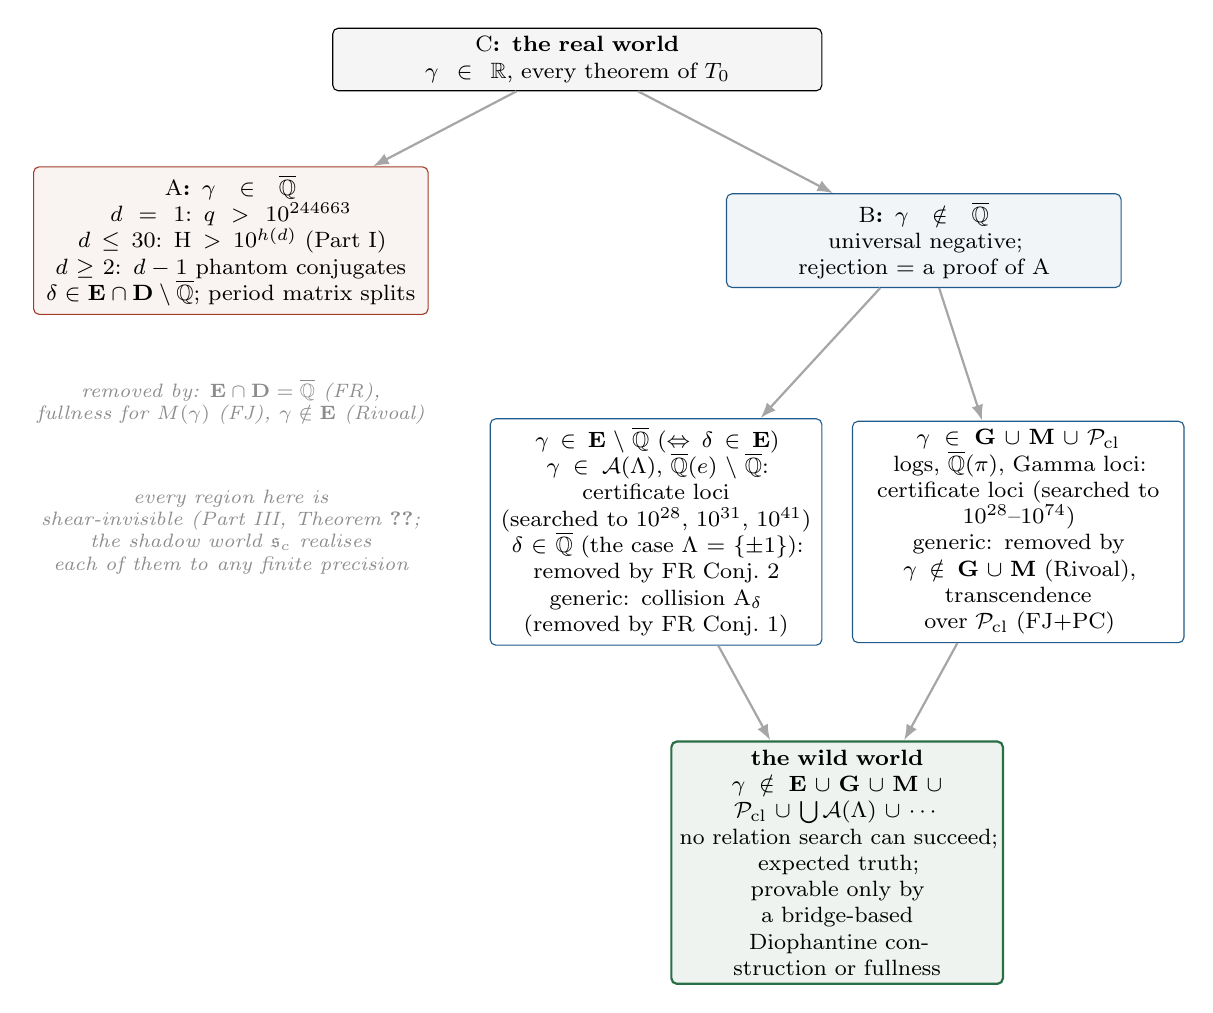
\begin{tikzpicture}[
  every node/.style={font=\footnotesize, align=center},
  box/.style={draw, rounded corners=2pt, inner sep=3pt, text width=#1, fill=white},
  edge/.style={-{Latex[length=2mm]}, thick, gray!70},
  lab/.style={font=\scriptsize\itshape, text=gray!90, align=center}]
\node[box=60mm, fill=gray!8] (C) at (0,0) {\textbf{$\mathrm C$: the real world}\\ $\gamma\in\R$, every theorem of $\Tz$};
\node[box=48mm, draw=aworld, fill=aworld!6] (A) at (-4.4,-2.3) {\textbf{$\mathrm A$: $\gamma\in\Qbar$}\\
  $d=1$: $q>10^{244663}$\\ $d\le30$: $\Ht>10^{h(d)}$ (Part~I)\\ $d\ge2$: $d-1$ phantom conjugates\\
  $\delta\in\EE\cap\DD\setminus\Qbar$; period matrix splits};
\node[box=48mm, draw=bworld, fill=bworld!6] (B) at (4.4,-2.3) {\textbf{$\mathrm B$: $\gamma\notin\Qbar$}\\ universal negative;\\ rejection $=$ a proof of $\mathrm A$};
\node[lab] at (-4.4,-4.35) {removed by: $\EE\cap\DD=\Qbar$ (FR),\\ fullness for $M(\gamma)$ (FJ), $\gamma\notin\EE$ (Rivoal)};
\node[box=40mm, draw=bworld] (BE) at (1.0,-6.0) {\textbf{$\gamma\in\EE\setminus\Qbar$} ($\Leftrightarrow\delta\in\EE$)\\
  $\gamma\in\Aff(\Lambda)$, $\Qbar(e)\setminus\Qbar$: certificate loci\\ (searched to $10^{28}$, $10^{31}$, $10^{41}$)\\
  $\delta\in\Qbar$ (the case $\Lambda=\{\pm1\}$):\\ removed by FR Conj.~2\\
  generic: collision $\mathrm A_\delta$\\ (removed by FR Conj.~1)};
\node[box=40mm, draw=bworld] (BG) at (5.6,-6.0) {\textbf{$\gamma\in\GG\cup\MM\cup\mathcal P_{\mathrm{cl}}$}\\
  logs, $\Qbar(\pi)$, Gamma loci:\\ certificate loci (searched to\\ $10^{28}$--$10^{74}$)\\
  generic: removed by\\ $\gamma\notin\GG\cup\MM$ (Rivoal),\\ transcendence over $\mathcal P_{\mathrm{cl}}$ (FJ+PC)};
\node[box=40mm, draw=wild, fill=wild!8, thick] (W) at (3.3,-10.2) {\textbf{the wild world}\\ $\gamma\notin\EE\cup\GG\cup\MM\cup\mathcal P_{\mathrm{cl}}\cup\bigcup\Aff(\Lambda)\cup\cdots$\\
  no relation search can succeed;\\ expected truth;\\ provable only by a bridge-based\\ Diophantine construction or fullness};
\draw[edge] (C) -- (A);
\draw[edge] (C) -- (B);
\draw[edge] (B) -- (BE);
\draw[edge] (B) -- (BG);
\draw[edge] (BE) -- (W);
\draw[edge] (BG) -- (W);
\node[lab] at (-4.4,-6.0) {every region here is\\ shear-invisible (Part~III, Theorem~\ref{III:thm:density};\\
  the shadow world $\shear_c$ realises\\ each of them to any finite precision};
\end{tikzpicture}
\caption{The map of possible worlds for $\gamma$. Boxes are regions consistent with every
proved theorem; ``certificate'' regions are those in which a proved identity would make $\gamma$
visibly transcendental; ``removed by'' names the conjecture expected to empty a region. $\mathcal P_{\mathrm{cl}}$: classical periods; $\MM$: Mahler values;
$\Aff(\Lambda)$: the $\Ein$-hyperplanes of Proposition~\ref{IV:prop:dual}. The regions
overlap (a logarithm is a $G$-value); the map is a stratification by certificate type,
not a partition.}
\label{IV:fig:map}
\end{figure}

Three features of the map deserve a sentence each. First, the $\mathrm A$-world is a
\emph{single} region, but it is realised to every finite precision by a shadow world
(Section~\ref{IV:sec:A}); it is small in the sense of measure and large in the sense of
evidence. Second, every certificate region is countable, explicit, and searchable, and all
searches to date are negative; the regions are the ``visible'' transcendence of $\gamma$,
and their emptiness below $10^{28}$--$10^{74}$ is the only positive information the
$\mathrm B$-side has produced. Third, the wild world is the complement of everything
explicit; it is where the conjectures put $\gamma$, and it is where no search can reach.
The two-world programme, run for its own sake, ends by drawing this map rather than by
closing it.

\section{A curiosity: the engine ratios of Rivoal's forms}\label{IV:sec:ratios}

Part~III wrote Rivoal's forms as $L_n=\alpha_n+\beta_n\gamma$ with engine coefficients
$\alpha_n=a_n+c_ne\Ein(1)$, $\beta_n=b_n-ec_n$ and asked for sequences of engine ratios
$-\alpha_n/\beta_n$ converging to $\gamma$ with $|L_n|\le H_n^{-1-\varepsilon}$. Rivoal's own
forms provide an empirical sequence, far from that specification.

\begin{proposition}[Engine ratios]\label{IV:prop:ratios}
\textup{(Finite certificate; script \texttt{exp12}.)} The ratios
$r_n:=-\alpha_n/\beta_n\in\Q(e,\Ein(1))$ approach $\gamma$ numerically for $n\le39$,
equivalently $t_n:=e(\Ein(1)-r_n)$ approaches $\delta$, with
\[
 -\log_{10}|\gamma-r_n|=1.89,\ 2.70,\ 3.92,\ 4.89,\ 5.64\quad(n=5,10,20,30,39),
\]
and $-\log_{10}|\gamma-r_n|/\sqrt n$ increases slowly from $0.85$ to $0.90$.
Explicitly, with Rivoal's polynomials at $-1$ and $\rho_n=R_{n+1,0}(-1)/R_{n,0}(-1)$,
\begin{equation}\label{IV:eq:rn}
 r_n=\frac{C_{n+1}-\rho_nC_n}{B_{n+1}-\rho_nB_n},\qquad
 \gamma-r_n=e^{-1}\,\frac{(A_{n+1}-\rho_nA_n)-\delta(B_{n+1}-\rho_nB_n)}{B_{n+1}-\rho_nB_n}.
\end{equation}
Taking $|B_n(-1)|\approx H_n^{1/2}$ as the height of $t_n$, the Stieltjes convergents of
$\delta$ of the same height are far better: at height $10^{103}$, $|\delta-t_{39}|=10^{-5.2}$
against $|\delta-s_{137}/q_{137}|=10^{-13.2}$ (at the full height $H_{39}=10^{208}$ the gap
is larger still).
\end{proposition}
\begin{proof}
With $R_n=e^{-1}A_n+B_nE(-1)+C_n$, $E(-1)=-\Ein(1)$, $P_n=A_n-B_n\delta$, $Q_n=C_n-B_n\gamma$
one has $R_n=e^{-1}P_n+Q_n$, $L_n=P_{n+1}Q_n-P_nQ_{n+1}=e(R_{n+1}Q_n-R_nQ_{n+1})$ and
$\beta_n=e(B_{n+1}R_n-B_nR_{n+1})$ (Part~III, Proposition~\ref{III:prop:rivoal-tie}, eq.~\eqref{III:eq:rivoal-tie}); dividing gives \eqref{IV:eq:rn}
after substituting $Q_n=C_n-B_n\gamma$ and $Q_{n+1}-\rho_nQ_n=-e^{-1}(P_{n+1}-\rho_nP_n)$.
The numbers are the computation at $1300$ digits.
\end{proof}

The observed approach is slow, of the subexponential type $\exp(-c\sqrt n)$ that Part~III
found on the $D$-side (nothing is proved about it: no bound on $|L_n|/|\beta_n|$ is
available), and it is dominated by Stieltjes's convergents by eight orders of magnitude at
comparable height. The $E$-side, once forced to speak about $\gamma$ rather than
about $e\gamma+\delta$, speaks in the $D$-side's voice and less clearly. This is the tie
theorem seen from the other end.

\section{Questions each world asks next}\label{IV:sec:questions}

Questions, not targets. They are what the worlds, left to themselves, want to know.

\paragraph{The $\mathrm A$-world asks.}
\begin{enumerate}[label=(A\arabic*)]
\item What is the degree? Every certificate pushes the height of $P_\gamma$ up
($10^{89.8}$ for $d\le12$ at $1200$ digits, Section~\ref{IV:sec:A}, script \texttt{exp12b}); the
$\mathrm A$-world with $d=1$ has no phantoms and the largest bound ($q>10^{244663}$).
\item Are the phantom conjugates real or complex? Nothing constrains them; the camouflage
of Part~I has one real and ten complex phantoms, all of modulus about $2.7\cdot10^7$
(the eleven other roots of $x^{12}+6.2\cdot10^{81}x-3.6\cdot10^{81}\approx0$ lie near a
circle of radius $\Ht(P_c)^{1/11}$).
\item Where does the period conjecture fail? In the $\mathrm A$-world it fails at
$M(\gamma)$ (Remark~\ref{IV:rem:FJ}(b)), but in $\mathrm A$ the number $\gamma+\log\alpha$ is
transcendental for every algebraic $\alpha\ne1$ (Hermite--Lindemann applied to
$\log\alpha$), so along the family of Euler constants
$\gamma+\log\alpha$---which is the twist family, by Proposition~\ref{IV:prop:twist}(iii)---the
splitting at the level of periods happens at $\alpha=1$ only. Is there a motivic reason why
the split point of the family should be its base point?
\item Does the Galois norm $\Nm(E_1(1))=P_\gamma(\Ein(1))$ have a meaning? It is an
$E$-value with rational coefficients whose irrationality exponent is $2$; the
$\mathrm A$-world knows its degree but not its value.
\item The $p$-adic cousin: Diamond's $p$-adic Euler constant $\gamma_p$ has the same
unknown arithmetic nature, and the $p$-adic theory has a Baker-type statement (for a prime
$q$, at most one of the numbers $\gamma_p$, $\gamma_p(r,q)$, $1\le r<q$, is algebraic
\cite{MurtySaradha}) in place of Rivoal's disjunction.
Does a twist $\Gamma_{p,\tau}$ of Morita's $\Gamma_p$ play the role of
Proposition~\ref{IV:prop:twist} there, and is the $p$-adic two-world problem shear-invisible in
the same sense?
\end{enumerate}

\paragraph{The $\mathrm B$-world asks.}
\begin{enumerate}[label=(B\arabic*)]
\item Is $\delta$ algebraic? This is the one certificate world inside $\gamma\in\EE$ not yet
removed by a theorem (only by Conjecture~2 of \cite{FRmixed}); a relation would give
$\gamma=\Ein(1)-\delta/e$ explicitly.
\item Which certificate locus is most plausible? None is expected to contain $\gamma$; but
the $\Ein$-hyperplanes are the only loci that the $\mathrm A$-world's own theorems point
to.
\item In the wild world, what is the irrationality exponent of $\gamma$? Expected $2$,
consistent with the $2910$ computed partial quotients (Part~I, Table~\ref{I:tab:cf}; no theorem gives
any bound at all.
\item Does the wild world have an internal structure? Part~III's hierarchy
$\mathrm X(V)$ grades it linearly; the twist of Section~\ref{IV:sec:twist} suggests grading it
by which normalisations of $\Gamma$ (functional equation, reflection, multiplication) a
statement uses.
\end{enumerate}

\paragraph{Both worlds ask.} Whether the unipotent matrices $D_\tau$ of
Remark~\ref{IV:rem:FJ}(c) are $\C$-points of the motivic Galois group of the polyexponential
tower. If they are, the two-model theorem is a theorem about the Galois torsor, and the
whole series of notes has been describing a single orbit.

\section{Computations for Part~IV}\label{IV:sec:computations}

Scripts (Python~3.11, \texttt{mpmath}~1.3, \texttt{sympy}~1.14, \texttt{fpylll}~0.6.4),
archived with outputs.
\begin{itemize}[leftmargin=*]
\item \texttt{exp12\_two\_worlds.py}: engine ratios from the exact coefficients of Part~I's
Rivoal forms and Stieltjes convergents of comparable height (Proposition~\ref{IV:prop:ratios});
the shadow world of the degree-$12$ camouflage (root by Newton at $1300$ digits, shadow
constants, $F_c(1)$, blindness of the forms, Galois norm and conjugate shadows, certified
lattice searches on $c$ and $\gamma$); the certificate zoo (Proposition~\ref{IV:prop:zoo}).
\item \texttt{exp12b\_find\_camouflage.py}: certified searches on $c$ and $\gamma$ at
$300$--$1200$ digits, with a candidate relation accepted only if it vanishes to $3p$ digits
and compared exactly with $P_c$.
\item \texttt{exp12c\_camouflage\_duality.py}: the roots $c_p$ of the certificate vectors,
with exact re-verification of the reductions and an irreducibility check of $Q_p$
(Proposition~\ref{IV:prop:duality}). The detector of \texttt{exp12} (inherited from Part~II)
reports only relations with coefficients below $10^6$, which is why its $1100$-digit run on
$c$ prints no relation although $b_1$ is $P_c$; \texttt{exp12b} uses the uncapped test.
\end{itemize}
Lattice reductions use \texttt{fplll} and are re-verified exactly (unimodularity by
Bareiss, the $(0.99,0.51)$ reduction conditions in rational arithmetic) as in Parts~I--II.
The only non-exact inputs are the values of $\gamma$, $e$, $\pi$, $\log p$, $\Gamma(1/3)$,
$\Gamma(1/4)$, $\Ein(\lambda)$, $E_1(1)$ supplied by \texttt{mpmath}. Run times: under ten
minutes in total.


\part{Forgeries, twists and the $\delta$-world}
\begin{partsummary}{V}
Three things from Part~IV are grown here. (1) The camouflage--certificate duality is
extended from the algebraic world to the certificate worlds of the map: at precision $p$,
the lattice vector that certifies ``$\gamma$ is not on this locus below height
$\approx10^{p/(m+1)}$'' is, read backwards, an explicit member of the locus within
$10^{-p}$ of $\gamma$. We exhibit the resulting \emph{gallery of forgeries}: rational,
quadratic and cubic algebraic numbers, a logarithm of an algebraic number, an element of
$\Q+\Q\log2+\dots+\Q\log7$, numbers cubic over $\Q(\pi)$ and over $\Q(e)$, an explicit
$E$-value on an $\Ein$-hyperplane, and an element of $\Q+\Q\pi+\Q\Gamma(\tfrac14)$, all
agreeing with $\gamma$ to $30$ digits with heights of $3$--$14$ digits; the same at $100$
digits, with a degree-$12$ algebraic number added. Their heights obey
$\Ht\approx10^{p/(m+1)}$ uniformly across the worlds, and the approximation exponents of
$\gamma$ by algebraic numbers of degree $d\le12$ are $d+1$ to within $1.1\%$ at $300$
digits: no finite observation prefers any world, quantitatively. (2) The twist $\Gamma_\tau$ is extended to
the incomplete Gamma function and to the mixed values of Fischler--Rivoal: the
residue-normalised twist $\widetilde\Gamma_\tau(a)=e^{-\tau a}\Gamma(a)$ gives
$\widetilde\Gamma_\tau(a,z)=e^{-\tau a}\Gamma(a)-\gamma(a,z)$ with
$\widetilde\Gamma_\tau(0,z)=E_1(z)-\tau$, regular at $a=0$ but, for real $\tau\ne0$, at no
other non-positive integer; in $\Gamma^{(s)}(a)=(-1)^ss!\,E_{a,s+1}(-1)+e^{-1}f_{a,s+1;0}(1)$
the $E$-side is fixed and the $D$-side moves by $e\,(\Gamma_\tau^{(s)}(a)-\Gamma^{(s)}(a))$,
which is $e$ times a $\Q[\tau]$-combination of Gamma derivatives at $a=1$ and involves
$e^{\tau(1-a)}$ elsewhere; for algebraic $\tau$ the twisted mixed values stay in the ring
$\Vring=\Sring\cdot\EE$ of Fischler--Rivoal. On the $\tau$-line, the worlds $\mathrm A$,
``$\delta\in\Qbar$'' and ``$e^\gamma\in\Qbar$'' are the statements that a coordinate of the
twisted system vanishes at some $\tau$ in $\Qbar$, $e^{-1}\Qbar$ or $\log\Qbar^\times$
respectively, and $\gamma+\log\alpha\in\Qbar$ for at most one $\alpha$, unconditionally.
(3) The $\delta$-world ($\delta\in\Qbar$), the one certificate world inside $\gamma\in\EE$
that no theorem removes, is given its certificate ($\delta$ satisfies no relation of degree
$\le12$ below $10^{20.6}$), its forgery, and its phantoms: shears by $\tau\in e^{-1}\Qbar$.
\end{partsummary}


\section{What grows from what}\label{V:sec:intro}

Part~IV, Proposition~\ref{IV:prop:duality}, observed that the lattice vector certifying ``no algebraic
relation of degree $\le12$ for $\gamma$ below height $\approx10^{p/13}$'' is the minimal polynomial
of an algebraic number within $10^{-p}$ of $\gamma$. Part~IV, Section~\ref{IV:sec:B}, listed the
certificate loci of the $\mathrm B$-world. Section~\ref{V:sec:gallery} puts the two together.
Part~IV, Section~\ref{IV:sec:twist}, identified the shear with the twist $\Gamma_\tau$; Section~\ref{V:sec:twist}
lets the twist act on everything else that carries a Gamma function. Part~IV, question
(B1), asked about the $\delta$-world; Section~\ref{V:sec:delta} answers what can be answered.

\section{The gallery of forgeries}\label{V:sec:gallery}

\subsection{Construction}

Fix a \emph{world} $W$ given by a finite list $x_0,\dots,x_m$ of real numbers containing
$\gamma$, or containing the powers of $\gamma$ (or of $e^\gamma$), such that a proved
relation $\sum k_ix_i=0$ with the coefficient of the $\gamma$-part nonzero would exhibit
$\gamma$ as an explicit member of $W$. The certified lattice search of Parts~I--II at $p$
digits returns a first vector $b_1=(k_0,\dots,k_m)$ with $|\sum k_ix_i|\lesssim\|b_1\|/N$,
$N=10^p/2$, and $\|b_1\|\approx10^{p/(m+1)}$. Solving the near-relation for the
$\gamma$-part produces a number $v_W$ of the world $W$ with
\begin{equation}\label{V:eq:forgery}
 |\gamma-v_W|\approx10^{-p},\qquad \Ht(v_W)\approx10^{p/(m+1)} ,
\end{equation}
which we call the \emph{forgery of $\gamma$ in $W$ at precision $p$}. The same vector
$b_1$ certifies that $\gamma$ satisfies no relation in $W$ below height
$\|b_1\|/(\alpha^{m/2}(m+1)\sqrt{m+2})$ (Part~II, Section~\ref{II:sec:probes}, which is $10^{1.5}$ to
$10^{2.5}$ below $\Ht(v_W)$. The forgery is verified to be different from $\gamma$ at
$3p+100$ digits, and it is a transcendental number whenever the theorem attached to $W$
applies to it (checked case by case in Table~\ref{V:tab:gallery30}). For the
$\Ein$-hyperplane $\Aff(\Lambda)$ of Part~IV the search is run on the weight-one basis
$\gamma-\Ein(1)$, $1$, $e^{\pm1}$, $e^{\pm2}$, $\Ein(-1)-\Ein(1)$, $\Ein(2)-\Ein(1)$, so that
the forgery has $\Ein$-weight exactly $1$; the search on the full span $V(\Lambda)$ (the
window of Part~IV's zoo) gives a forgery of weight $\ne1$, also listed.

\begin{table}[t]
\centering\footnotesize
\caption{Forgeries of $\gamma$ at $30$ digits (scripts \texttt{exp13b}, \texttt{exp13c}). $v$ is
the number defined in the second column; $|\gamma-v|$ is computed at $190$ digits. In every
row $v\ne\gamma$.}
\label{V:tab:gallery30}
\begin{tabular}{@{}>{\raggedright\arraybackslash}p{17mm}>{\raggedright\arraybackslash}p{86mm}r>{\raggedright\arraybackslash}p{22mm}@{}}
\toprule
world & forgery $v$ & $\log_{10}|\gamma-v|$ & $v\notin\Qbar$ by\\
\midrule
rational & $12668145165383/21946987817013$ & $-28.4$ & (algebraic)\\
quadratic & root near $0.577$ of $1825589204x^2-2377304883x+763971598$ & $-28.4$ & (algebraic)\\
cubic & root near $0.577$ of $10806397x^3-12006300x^2+5013002x-971587$ & $-28.7$ & (algebraic)\\
exponential & $\log\alpha$, $\alpha$ the real root near $1.781$ of
 $3899x^6-1521x^5+501x^4-6072x^3-15134x^2-13627x+4341$ (irreducible) & $-31.0$ & Hermite--Lindemann\\
logarithmic & $(19275-19985\log2+50615\log3+11986\log5-27071\log7)/47888$ & $-29.8$ & Hermite--Lindemann\\
$\pi$-locus & root near $0.577$ of $170x^3+(334\pi-436)x^2+(116-627\pi-75\pi^2)x$ $+(173-305\pi+113\pi^2+30\pi^3)$ (irreducible in $\Q[x,y]$) & $-30.3$ & Lindemann\\
$e$-locus & root near $0.577$ of $-312x^3-(36+76e)x^2-(383+157e+325e^2)x$ $+(210+742e+292e^2-119e^3)$ (irreducible in $\Q[x,y]$) & $-31.5$ & Hermite\\
$\Ein$-hyperplane (weight $1$) & $\bigl(-2521+721e-1376e^{-1}+106e^{2}+2322e^{-2}$ $+3798\Ein(1)-315\Ein(-1)-1968\Ein(2)\bigr)/1515$ & $-29.6$ & Beukers\\
$\Ein$-span (weight $-593/720$) & $\bigl(281+976e+338e^{-1}-260e^{2}+1407e^{-2}$ $+778\Ein(1)-105\Ein(-1)-1266\Ein(2)\bigr)/720$ & $-29.7$ & Beukers\\
$\Gamma(\tfrac14)$-locus & $\bigl(-25383337+17880293\,\pi-7430501\,\Gamma(\tfrac14)\bigr)/6668499$ & $-29.7$ & Chudnovsky\\
\bottomrule
\end{tabular}
\end{table}

\begin{proposition}[The gallery]\label{V:prop:gallery}
\textup{(Finite certificate; scripts \texttt{exp13}, \texttt{exp13b}, \texttt{exp13c}.)}
Table~\ref{V:tab:gallery30} lists forgeries of $\gamma$ at $30$ digits in ten worlds;
Table~\ref{V:tab:gallery100} the heights at $100$ digits. In each transcendental row the
forgery is a transcendental number, by the theorem named, and in each row $v\ne\gamma$. The
bivariate polynomials of the $\pi$- and $e$-rows are irreducible in $\Q[x,y]$, so those
forgeries have degree exactly $3$ over $\Q(\pi)$, resp.\ $\Q(e)$. The heights follow
\eqref{V:eq:forgery}: at $p=60,100,200,300$ the ratio $p/\log_{10}\Ht(v_W)$ equals $m+1$ to
within $3\%$ for $p\ge100$ (Table~\ref{V:tab:law}).
\end{proposition}
\begin{proof}
The construction and the verification at $3p$ digits are the computation. Transcendence:
$\log\alpha$ with $\alpha\ne1$ algebraic is transcendental (Hermite--Lindemann);
so is $q_0+q_1\log r$ for rational $q_0$, $q_1\ne0$ and rational $r\ne1$ (here
$q_1=1/47888$ and $r=2^{-19985}3^{50615}5^{11986}7^{-27071}$);
a root $v$ of $P(x,\pi)=0$ is algebraic only if $P(v,y)\equiv0$, i.e.\ only if the minimal
polynomial of $v$ divides every coefficient of $P$ as a polynomial in $y$, which is excluded
by irreducibility (same for $e$); the two $\Ein$ forgeries are $\Q$-linear combinations of
$1,e^{\pm1},e^{\pm2},\Ein(\pm1),\Ein(2)$ with nonzero $\Ein$ coefficients, hence not
algebraic, because these eight numbers are linearly independent over $\Qbar$ (Part~IV,
Lemma~\ref{IV:lem:multipoint} with $\Lambda=\{1,-1,2\}$, $M=\{\pm1,\pm2\}$, and Beukers' theorem
\cite{Beukers}); the Gamma forgery is algebraic only if $17880293\pi-7430501\Gamma(\tfrac14)$
is, contradicting the algebraic independence of $\pi$ and $\Gamma(\tfrac14)$ \cite{Chudnovsky}.
\end{proof}

\begin{table}[t]
\centering\small
\caption{Heights of the forgeries at $100$ digits (script \texttt{exp13}); $m+1$ is the
number of basis elements, $p/(m+1)$ the Dirichlet prediction for $\log_{10}\Ht$.}
\label{V:tab:gallery100}
\begin{tabular}{@{}lrrrr@{}}
\toprule
world & $m+1$ & $\log_{10}\Ht(v)$ & $p/(m+1)$ & $\log_{10}|\gamma-v|$\\
\midrule
rational & 2 & 49.6 & 50.0 & $-100.3$\\
quadratic & 3 & 33.1 & 33.3 & $-100.3$\\
degree $12$ & 13 & 7.5 & 7.7 & $-99.0$\\
exponential (degree $\le6$) & 7 & 14.2 & 14.3 & $-100.6$\\
logarithmic & 6 & 16.6 & 16.7 & $-99.4$\\
$\pi$-locus (degree $\le3$) & 10 & 9.9 & 10.0 & $-100.4$\\
$e$-locus (degree $\le3$) & 10 & 9.9 & 10.0 & $-100.3$\\
$\Ein$-hyperplane (weight $1$) & 8 & 12.4 & 12.5 & $-99.3$\\
$\Ein$-span & 9 & 10.8 & 11.1 & $-99.7$\\
$\Gamma(1/4)$-locus & 4 & 24.6 & 25.0 & $-98.9$\\
\bottomrule
\end{tabular}
\end{table}

\begin{table}[t]
\centering\small
\caption{The law $\Ht(v_W)\approx10^{p/(m+1)}$: the ratio $p/\log_{10}\Ht(v_W)$ at four
precisions (scripts \texttt{exp13}, \texttt{exp13c}), to be compared with $m+1$.}
\label{V:tab:law}
\begin{tabular}{@{}lrrrrr@{}}
\toprule
world & $m+1$ & $p=60$ & $p=100$ & $p=200$ & $p=300$\\
\midrule
quadratic & 3 & 3.13 & 3.02 & 3.04 & 3.01\\
degree $12$ & 13 & 13.53 & 13.34 & 13.22 & 13.13\\
exponential & 7 & 7.23 & 7.04 & 7.04 & 7.02\\
logarithmic & 6 & 6.13 & 6.04 & 6.05 & 6.04\\
$\Ein$-hyperplane (weight $1$) & 8 & 8.09 & 8.07 & 8.04 & 8.05\\
$\Ein$-span & 9 & 9.00 & 9.25 & 9.08 & 9.11\\
$\Gamma(1/4)$-locus & 4 & 4.06 & 4.06 & 4.00 & 4.02\\
\bottomrule
\end{tabular}
\end{table}

\subsection{What the gallery says}

Part~I's symmetry of finite observations (Theorem~\ref{I:thm:symmetry} there) was a statement about the
algebraic world. The gallery is its quantitative form for every world at once: at
precision $p$, $\gamma$ is a member of each world $W$ at the cost $10^{p/(m+1)}$, the cost
depends on $W$ only through the dimension $m+1$ of its basis, and no world is cheaper than
its dimension predicts. A world in which $\gamma$ \emph{really} lived would announce itself
by a forgery far cheaper than $10^{p/(m+1)}$---a coefficient vector that stops growing as
$p$ increases. Table~\ref{V:tab:law} shows no such world among its seven to $300$ digits,
and Table~\ref{V:tab:gallery100} none among the ten to $100$ digits.

\begin{proposition}[Approximation exponents of $\gamma$]\label{V:prop:wirsing}
\textup{(Finite certificate; script \texttt{exp13}.)} For $1\le d\le12$ let $H_d$ be the
height of the degree-$d$ forgery at $p=300$ and $w_d:=300/\log_{10}H_d$. Then
\[
 (w_d)_{d=1}^{12}=2.00,\ 3.01,\ 4.02,\ 5.03,\ 6.03,\ 7.07,\ 8.08,\ 9.10,\ 10.09,\ 11.10,\ 12.13,\ 13.13 ,
\]
i.e.\ $w_d=d+1$ to within $1.1\%$. In Koksma's normalisation ($|\gamma-c|\le\Ht(c)^{-w^*_d-1}$)
this reads $w_d^*(\gamma)=d$, which is the value for almost every real number
(Sprind\v zuk; see \cite{Bugeaud}); $\gamma$ behaves, to $300$ digits and degree $12$,
like almost every real number. ($H_d$ is the LLL height, an upper bound for the minimal
height within the factor $\alpha^{d/2}\sqrt{d+1}$, about $10^{2.5}$ at $d=12$; the
conclusion is insensitive to this, since a world in which $\gamma$ really lived would show
a vector that stops growing with $p$.)
\end{proposition}

The two worlds read this differently and agree on its content. In $\mathrm B$ (wild), the
expected value is $w_d=d+1$ for all $d$: $\gamma$ is expected to be an $S$-number of type $1$
in Mahler's classification, like almost all reals. In $\mathrm A$ with $[\Q(\gamma):\Q]=d_0$,
Schmidt's theorem on the approximation of algebraic numbers by algebraic numbers of bounded
degree \cite{Schmidt1971} gives $w_d=d+1$ for $d<d_0$, while for $d\ge d_0$ the polynomial
$P_\gamma$ itself is a forgery of infinite precision and the finite-$p$ ratio
$p/\log_{10}H_d$ would grow without bound; the table therefore says $d_0>12$ or
$\Ht(P_\gamma)>10^{20.6}$ (the certified bound at $300$ digits), which is weaker than the
$1200$-digit certificate of Part~IV. Neither world is contradicted, and neither could be:
the table is the shadow of $\mathrm A$ and of $\mathrm B$ alike.

\section{The twist, extended}\label{V:sec:twist}

Part~IV defined $\Gamma_\tau(s)=\Gamma(s)e^{\tau(1-s)}$, with $\Gamma_\tau(1)=1$, Euler
constant $\gamma+\tau$, and functional equation $\Gamma_\tau(s+1)=se^{-\tau}\Gamma_\tau(s)$.
Here it acts on the incomplete Gamma function, on the mixed values of Fischler--Rivoal, and
on the whole twisted system as a line.

\subsection{The incomplete Gamma function}

Write $\gamma(a,z)=\int_0^zt^{a-1}e^{-t}dt=z^a\sum_{n\ge0}(-z)^n/(n!(a+n))$ for the lower
incomplete Gamma function (meromorphic in $a$, poles at $a=-n$ with residues $(-1)^n/n!$),
so that $\Gamma(a,z)=\Gamma(a)-\gamma(a,z)$ is entire in $a$ and $\Gamma(0,z)=E_1(z)$.

\begin{proposition}[Twisted incomplete Gamma]\label{V:prop:incgamma}
Let $\widetilde\Gamma_\tau(a):=e^{-\tau a}\Gamma(a)=e^{-\tau}\Gamma_\tau(a)$ (residue $1$ at
$a=0$) and $\widetilde\Gamma_\tau(a,z):=\widetilde\Gamma_\tau(a)-\gamma(a,z)$. Then:
\begin{enumerate}[label=(\roman*)]
\item $\widetilde\Gamma_\tau(a,z)$ is regular at $a=0$ and
$\widetilde\Gamma_\tau(0,z)=E_1(z)-\tau=-(\gamma+\tau)-\log z+\Ein(z)$: the twisted
$E_1$ is the sheared $Z_\lambda$ of Part~I, and the connection formula
$\Ein(z)=(\gamma+\tau)+\log z+\widetilde\Gamma_\tau(0,z)$ holds with the twisted Euler
constant.
\item At $a=-n$, $n\ge1$, $\widetilde\Gamma_\tau(a,z)$ has a simple pole with residue
$(-1)^n(e^{\tau n}-1)/n!$, nonzero for real $\tau\ne0$: the twist respects the Stokes
structure of the incomplete Gamma function at $a=0$ only. Within the family of twists $f(a)\Gamma(a)$ with constant
functional-equation factor $f(a+1)/f(a)=c$, regularity of $f\Gamma-\gamma(\cdot,z)$ at all
$a\in-\mathbb N$ forces $f(-n)=1$ for all $n$, hence $c=1$: such a twist cannot change
the functional-equation constant, and if it shifts the Euler constant it does so through a
$1$-periodic factor, which by Bohr--Mollerup destroys log-convexity.
\item The residue normalisation ($\Res_{a=0}=1$) and the value normalisation
($\Gamma_\tau(1)=1$) differ by the constant $e^{\tau}$; for real $\tau$ they agree only
for $\tau=0$, which is the functional equation $\Gamma(1)=\Res_{a=0}\Gamma(a)$ once more.
\end{enumerate}
\end{proposition}
\begin{proof}
(i) $e^{-\tau a}\Gamma(a)=(1-\tau a+O(a^2))(a^{-1}-\gamma+O(a))=a^{-1}-\gamma-\tau+O(a)$ and
$\gamma(a,z)=a^{-1}+\log z-\Ein(z)+O(a)$ (from $z^a/a=a^{-1}+\log z+O(a)$ and the series
with $n\ge1$); subtract. (ii) The residue of $e^{-\tau a}\Gamma(a)$ at $-n$ is
$e^{\tau n}(-1)^n/n!$, that of $\gamma(a,z)$ is $(-1)^n/n!$. If $f$ is meromorphic, regular
at $-\mathbb N$, and $f(a)\Gamma(a)$ satisfies $f(a+1)/f(a)=c$, regularity of
$f\Gamma-\gamma(\cdot,z)$ at $-n$ means
$f(-n)(-1)^n/n!=(-1)^n/n!$, so $f(-n)=1$ for all $n\ge0$ and $c=f(-n+1)/f(-n)=1$; then
$f$ is $1$-periodic with $f(1)=1$, and the Euler constant of $f\Gamma$ is $\gamma-f'(1)$.
(iii) is the definition.
\end{proof}

The numerical check of (i) is in script \texttt{exp13}: at $a=10^{-24}$ the difference
$\widetilde\Gamma_\tau(a,z)-(E_1(z)-\tau)$ is $2.8\cdot10^{-25}$ ($\tau=0.3$, $z=1.7$).

\subsection{The mixed values of Fischler--Rivoal}

Recall (Part~II, Theorem~\ref{II:thm:FR2018}(iii)) the decomposition
\begin{equation}\label{V:eq:mixed}
 \Gamma^{(s)}(a)=(-1)^ss!\,E_{a,s+1}(-1)+e^{-1}f_{a,s+1;0}(1),\qquad
 E_{a,s}(z)=\sum_{n\ge0}\frac{z^n}{n!\,(n+a)^s},\quad f_{a,s+1;0}(1)\in\DD ,
\end{equation}
for rational $a>0$ and $s\ge0$; at $(a,s)=(1,1)$ it is $\gamma=\Ein(1)-e^{-1}\delta$.

\begin{proposition}[The twist on mixed values]\label{V:prop:mixed}
Under $\Gamma\mapsto\Gamma_\tau$, the $E$-side of \eqref{V:eq:mixed} is unchanged and the
$D$-side becomes
\begin{equation}\label{V:eq:Dshift}
 f^\tau_{a,s+1;0}(1)=f_{a,s+1;0}(1)+e\bigl(\Gamma_\tau^{(s)}(a)-\Gamma^{(s)}(a)\bigr),\qquad
 \Gamma_\tau^{(s)}(a)=e^{\tau(1-a)}\sum_{j=0}^s\binom sj(-\tau)^j\,\Gamma^{(s-j)}(a).
\end{equation}
At $a=1$ the shift is $e$ times the $\Q[\tau]$-combination $\sum_{j\ge1}\binom sj(-\tau)^j\Gamma^{(s-j)}(1)$;
for $(a,s)=(1,1)$ it is $-e\tau$, i.e.\ $\delta\mapsto\delta-e\tau$, the shear. For $a\ne1$
it involves the factor $e^{\tau(1-a)}$. Consequently, for algebraic $\tau$ and rational $a$,
the twisted values $\Gamma_\tau^{(s)}(a)$ lie in $\Vring=\Sring\cdot\EE$ (an element of
$\Sring$ times an $E$-value), and the twisted mixed values $f^\tau_{a,s+1;0}(1)$ stay in
$\Vring$: Fischler--Rivoal's containment $\DD\subset\Vring$ (Part~II, Theorem~\ref{II:thm:FR2018}(i)) is
twist-compatible. Nothing places the twisted values in $\Sring$ itself.
\end{proposition}
\begin{proof}
Leibniz' rule for $\Gamma(a)e^{\tau(1-a)}$; then solve \eqref{V:eq:mixed} for $f$. The ring
statement: $\Gamma^{(k)}(a)\in\Sring$, $e^{\tau(1-a)}\in\EE$ for algebraic $\tau$ and
rational $a$, $e\in\EE$, $f\in\DD\subset\Vring$, and $\Vring$ is a ring.
\end{proof}

The identity in \eqref{V:eq:Dshift} is verified numerically at $a=1$ for $s=1,2,3$ at $60$
digits in script \texttt{exp13}. Its meaning is the one Part~I assigned to the shear in the language
of Stokes framings \cite{K002}: the $E$-functions $E_{a,s}$ are the ``series side'' and are
fixed; the Gamma derivatives are the ``Stokes side'' and move. In the $\mathrm A$-world with
$\tau=\sigma(\gamma)-\gamma$, the conjugate mixed values at $a=1$ are $\Qbar$-combinations of
the true ones, consistent with $\Gamma^{(s)}(1)\in\Q[\gamma,\zeta(2),\zeta(3),\dots]$; at
$a\ne1$ they pick up the $E$-values $e^{\tau(1-a)}$: the phantom Gamma functions have
phantom values at the rationals which are true Gamma values times exponentials of algebraic
numbers.

\subsection{The $\tau$-line}

The twisted system is a line through the true system:
\[
 \tau\ \longmapsto\ \Bigl(\gamma+\tau,\ \ \delta-e\tau,\ \ E_1(\lambda)-\tau,\ \ \Gamma(a)e^{\tau(1-a)},\ \
 \omega_{\lambda,r}\text{ with }P_r(\lambda e^{\tau};\gamma)\Bigr),\qquad\tau\in\C .
\]
Each coordinate is an affine, exponential or polynomial function of $\tau$, every
connection identity holds along the whole line, and Part~I's two-model theorem says that
the established theorems hold along the real segment of the line permitted by the
enclosures they use, and along the whole line when they use only the connection
identities. The worlds of the map (Part~IV, Figure~\ref{IV:fig:map} are
statements about \emph{where on the line a coordinate vanishes}:
\begin{itemize}[leftmargin=*]
\item $\mathrm A$: the $\gamma$-coordinate vanishes at some $\tau\in\Qbar$.
\item the $\delta$-world ($\delta\in\Qbar$): the $\delta$-coordinate vanishes at some
$\tau\in e^{-1}\Qbar$.
\item the exponential certificate world ($e^\gamma\in\Qbar$): the $\gamma$-coordinate
vanishes at some $\tau\in\log\Qbar^\times\setminus\{0\}$.
\item the $\Ein$-hyperplane worlds: the $\gamma$-coordinate vanishes at some
$\tau\in-\Aff(\Lambda)$.
\end{itemize}
The sets $\Qbar$, $e^{-1}\Qbar$, $\log\Qbar^\times$, $\Aff(\Lambda)$ are countable with real
points dense in $\R$, and they are pairwise disjoint away from $0$ whenever a theorem says
so:
$\Qbar\cap\log\Qbar^\times=\{0\}$ (Hermite--Lindemann), $\Qbar\cap e^{-1}\Qbar=\{0\}$
(Hermite), $\Qbar\cap\Aff(\Lambda)=\varnothing$ (Beukers); whether
$e^{-1}\Qbar$ meets $\log\Qbar^\times$ is open (it asks whether $e^{\alpha/e}$ can be
algebraic). One unconditional consequence deserves its own line.

\begin{proposition}\label{V:prop:oneshift}
There is at most one $\alpha\in\Qbar^\times$ with $\gamma+\log\alpha\in\Qbar$. If it exists
and $\alpha=1$, world $\mathrm A$ holds; if it exists and $\alpha\ne1$, world $\mathrm B$
holds with the certificate $e^{\gamma}\in\Qbar^\times e^{\Qbar}$.
\end{proposition}
\begin{proof}
Two such $\alpha,\alpha'$ give $\log(\alpha/\alpha')\in\Qbar$, hence $\alpha=\alpha'$ by
Hermite--Lindemann. If $\alpha\ne1$ and $\gamma+\log\alpha=\beta\in\Qbar$, then
$\gamma=\beta-\log\alpha$ is transcendental, since otherwise $\log\alpha$ would be algebraic.
\end{proof}

\section{The $\delta$-world}\label{V:sec:delta}

The world ``$\delta\in\Qbar$'' is the one certificate region inside $\gamma\in\EE$ that no
proved theorem removes (Part~IV, Figure~\ref{IV:fig:map}: Rivoal's theorem removes only its intersection
with $\mathrm A$, and Fischler--Rivoal's Corollary~1 removes it under their Conjecture~2.
In it, $\gamma=\Ein(1)-\delta e^{-1}$ is an explicit $E$-value with coefficients in
$\Q(\delta)$, hence transcendental by Beukers' theorem, and the whole linear theory of
$\gamma$ against $E$-values is governed by the functional relations of the $E$-function
$F(z)=\Ein(z)-\delta e^{-z}$.

\begin{proposition}[The $\delta$-world's certificate, forgery and phantoms]\label{V:prop:delta}
\begin{enumerate}[label=(\roman*)]
\item \textup{(Finite certificate; script \texttt{exp13}.)} $\delta$ satisfies no integer
relation of degree $\le12$ with height below $10^{20.6}$ ($300$ digits). The certifying
vector is the (irreducible) minimal polynomial of a degree-$12$ algebraic number of height
$10^{22.8}$ within $10^{-298.8}$ of $\delta$: the $\delta$-world has its forgeries at the
same price as the others.
\item In the $\delta$-world with $d=[\Q(\delta):\Q]$, the Galois conjugates of the system
are the twists by $\tau_\sigma=(\delta-\sigma(\delta))e^{-1}\in e^{-1}\Qbar$: the conjugate
Euler constants $\gamma^{(\sigma)}=\Ein(1)-\sigma(\delta)e^{-1}$ are $E$-values, and they are
the Euler constants of $\Gamma_{\tau_\sigma}$, whose values at the integers are
$n!\exp\bigl(-n(\delta-\sigma(\delta))/e\bigr)$.
\item The $\delta$-world implies $\gamma\notin\Qbar$ (Rivoal), $\gamma\in\EE$,
$\gamma\in\Aff(\{1,-1\})$, and $\mathrm X(W)$ of Part~III fails; it is consistent with
$\EE\cap\DD=\Qbar$ (the collision $\delta\in\EE\cap\DD$ is at an algebraic point); of the
conjectures of \cite{FRmixed} it contradicts only Conjecture~2, and it contradicts Rivoal's
expectation $\gamma\notin\EE$ \cite{Rivoal2017}.
\end{enumerate}
\end{proposition}
\begin{proof}
(i) is the computation. (ii) $\gamma^{(\sigma)}-\gamma=(\delta-\sigma(\delta))e^{-1}=\tau_\sigma$,
and Part~IV, Proposition~\ref{IV:prop:twist}. (iii) $\gamma=\Ein(1)-\delta e^{-1}$ has $\Ein$-weight $1$ in
$V(\{1,-1\})$; the rest is Part~III, Theorem~\ref{III:thm:hierarchy} and Part~II, Definition~\ref{II:def:dichotomy}.
\end{proof}

The $\delta$-world is thus the mirror image of $\mathrm A$: there the phantoms are
algebraic shifts, here they are algebraic multiples of $e^{-1}$; there $\delta$ is a
transcendental $E$-value and $\gamma$ algebraic, here $\gamma$ is a transcendental $E$-value
and $\delta$ algebraic; the two worlds are exchanged by the connection formula and cannot
both hold (Rivoal's theorem). The $\mathrm A$-world's shadow systems and Galois norm have
their $\delta$-world counterparts ($P_\delta(e\Ein(1))=e^d\prod_\sigma\gamma^{(\sigma)}$, a
nonzero element of $\Q[e\Ein(1)]$); the $\delta$-world's Beukers theory is different in
shape, since there $\Ein(1)-\gamma\in\Qbar e^{-1}$ makes the family of Part~IV,
Theorem~\ref{IV:thm:Aworld}, dependent as soon as $-1\in\Lambda$.

\section{Questions}\label{V:sec:questions}

\begin{enumerate}[label=(Q\arabic*)]
\item Is there a world in which the forgeries are cheap? A finite basis $x_0,\dots,x_m$ of
explicit constants for which $p/\log_{10}\Ht(v)$ stays clearly above $m+1$ as $p$ grows
would be a discovery, whatever the world; the gallery is a template for looking, and the
$34$-element and $78$-monomial windows of Part~II are its largest instances so far
($\gamma$ has forgeries there of the predicted cost, and no cheaper).
\item The twist respects the Stokes structure of $\Gamma(a,z)$ at $a=0$ only
(Proposition~\ref{V:prop:incgamma}(ii)). Is there a deformation of the whole incomplete Gamma
family, non-constant in $a$, that shifts every Stokes constant consistently, and what
replaces the Euler constant along it?
\item The twisted Gamma values and mixed values land in $\Vring=\Sring\cdot\EE$
(Proposition~\ref{V:prop:mixed}), and nothing places them in $\Sring$. Is the
twist-compatibility of $\DD\subset\Vring$ a hint about which ring the $D$-values
``really'' live in?
\item Proposition~\ref{V:prop:oneshift} says that at most one algebraic rescaling
$\alpha$ makes $\gamma+\log\alpha$ algebraic. Is there any statement of the same shape for
the $\Ein$-hyperplanes, i.e.\ at most one point of $\bigcup_\Lambda\Aff(\Lambda)$ can equal
$\gamma$? (Yes, trivially, but the interesting version asks for a bound on the height of
that point in terms of $\Lambda$, which would be a Diophantine statement about $\gamma$ of
the kind Part~III found blocked.)
\end{enumerate}

\section{Computations for Part~V}\label{V:sec:computations}

Scripts (Python~3.11, \texttt{mpmath}~1.3, \texttt{sympy}~1.14, \texttt{fpylll}~0.6.4),
archived with outputs.
\begin{itemize}[leftmargin=*]
\item \texttt{exp13\_forgeries.py}: forgeries in nine worlds at $100$ digits with verification
at $300$ digits (Table~\ref{V:tab:gallery100}); the height law at $p=60,100,200,300$
(Table~\ref{V:tab:law}); Wirsing exponents $w_d$, $d\le12$, at $300$ digits
(Proposition~\ref{V:prop:wirsing}); the $\delta$-world certificate and forgery
(Proposition~\ref{V:prop:delta}); numerical checks of Propositions~\ref{V:prop:incgamma}(i)
and~\ref{V:prop:mixed}. All lattice reductions are re-verified exactly (unimodularity,
$(0.99,0.51)$ conditions) as in Parts~I--II; irreducibility and the absence of factors in
$x$ alone are checked with \texttt{sympy}.
\item \texttt{exp13b\_small\_forgeries.py}: the printable $30$-digit forgeries of
Table~\ref{V:tab:gallery30}, verified at $190$ digits.
\item \texttt{exp13c\_hyperplane\_forgery.py}: the weight-one $\Ein$-hyperplane forgeries at
$p=30$--$300$ and the irreducibility of the bivariate polynomials of the $\pi$- and
$e$-rows.
\end{itemize}
Run time: about $15$ minutes in total.


\part*{Conclusion}
\addcontentsline{toc}{part}{Conclusion}

\section{What the two worlds taught}\label{sec:conclusion}

The programme was to build inside $\mathrm A$ and inside $\mathrm B$ until the real
world rejected something. It did not, and Lemma~\ref{III:lem:bookkeeping} says why it
could not have done so cheaply: a rejection inside a world is a proof of the other world
under another name. What the programme produced instead is a description of the tools.

The description has one centre. Every established arithmetic theorem about $\gamma$ that
we could find reaches $\gamma$ through a connection formula, and is therefore blind to the
one-parameter family of \emph{twisted Gamma functions} $\Gamma_\tau(s)=\Gamma(s)e^{\tau(1-s)}$,
whose Euler constants $\gamma+\tau$ fill the real line. The two-model theorem
(Theorem~\ref{I:thm:two-models}) is the logical form of this blindness; the density
obstruction (Theorem~\ref{III:thm:density}) is its extension to every arithmetic class;
the tie theorem (Theorem~\ref{III:thm:tie}) is its quantitative form on linear forms,
where it caps the exponent of shear-invariant families at $1$ and explains why Rivoal's
forms sit at $\tfrac12$ with $b_n/c_n\to e$; the twist (Proposition~\ref{IV:prop:twist})
is its function-theoretic form, in which the only things pinning $\tau=0$ are the
normalisations of the Gamma function---$\Gamma(2)=1$, the reflection and multiplication
constants, Stirling's formula, the exponential in Euler's integral---none of which enters
the transcendence machinery. In the language of Fischler and Rivoal, the twist fixes the
$E$-side and moves the $D$-side; in the language of the companion manuscript \cite{K002},
it is the Stokes-framing shear on numbers; in the language of Fres\'an and Jossen, it is
a $\C$-linear change of de Rham basis that fixes the period $\Ein(1)$ of the cycle
$\sigma_1+\sigma_2$, and the $\mathrm A$-world is the statement that a $\Qbar$-linear one
exists which kills the period of $\sigma_1$ while, by their theorem, the motive itself
does not split.

Around this centre the worlds grew. The $\mathrm A$-world has honest $E$-values for all
its shadow constants, a Galois theory with phantom conjugates that are Euler constants of
twisted Gamma functions without an analytic definition of their own, a Galois norm, and
a Beukers theory whose sentences $\mathrm C$ cannot at present prove; its Diophantine
consequences---the floor, the forced approximations along the definitions, the rigidity
$\mu(\delta)=2$---are all expected to be true, and its non-Diophantine
consequences---$\delta\in\EE\cap\DD$, the split period matrix, the collision in the
tower---are all expected to be false, each rejected by a standing conjecture evaluated at
one element. The $\mathrm B$-world is a universal negative whose only positive content
is the list of certificate loci dual to the $\mathrm A$-world's theorems; on each of them
$\gamma$ has a forgery at the uniform price $\Ht\approx10^{p/(m+1)}$ and no cheaper, and
the certified searches find $\gamma$ on none of them. The expected truth is the wild
world, in which every finite search is a search of an empty region.

Three things would change this picture, and they are the targets the programme leaves
behind. A sequence of integer forms in $1,\gamma,\delta$ smaller than its own tie defect,
with a proof that reaches $\gamma$ through a bridge (Specification~\ref{III:spec}), would
be the first Diophantine construction that the shear does not neutralise; the
$E$-side produces tied forms, the $D$-side untied but large ones, and the two have not
been combined. The point conjecture $\mathrm B_\delta$: $\delta\in\EE\Rightarrow\delta\in\Qbar$
(Definition~\ref{II:def:dichotomy}, Proposition~\ref{II:prop:position}) would reject the
collision and, with $\delta\notin\Qbar$, give the middle term of the linear hierarchy of
Theorem~\ref{III:thm:hierarchy}. Fullness of the period realisation for the
Euler--Mascheroni motive would reject the split period matrix. Below all three sits the
weakest unproved sentence above $\mathrm B$, the linear independence of $1,e,e\gamma$
over $\Qbar$, for which the ledger records no route at all.

We end where the session ended: not with a proof, but with a map on which the proof would
have to be found, drawn to the precision the available instruments allow.

\appendix

\section{Computational archive}\label{app:archive}

All computations were performed with Python~3.11, \texttt{mpmath}~1.3, \texttt{sympy}~1.14
and \texttt{fpylll}~0.6.4 (\texttt{fplll}~5), on one core. Lattice reductions are
re-verified exactly (unimodularity by Bareiss, the $(0.99,0.51)$ reduction conditions in
rational arithmetic) and the height bounds are those of Part~I, Section~\ref{I:sec:computations},
and Part~II, Section~\ref{II:sec:probes}. The only non-exact inputs are the values of the
classical constants supplied by \texttt{mpmath} at $300$--$1660$ digits; all heights,
coefficients and continued-fraction data are exact integers. The archive (scripts,
logs, JSON outputs, and the \LaTeX\ sources of the five parts) accompanies this paper.

\begin{footnotesize}
\begin{longtable}{@{}>{\raggedright\arraybackslash}p{47mm}>{\raggedright\arraybackslash}p{77mm}>{\raggedright\arraybackslash}p{24mm}@{}}
\caption{Scripts of the archive.}\label{tab:archive}\\
\toprule
script & content & used in\\
\midrule
\endfirsthead
\toprule
script & content & used in\\
\midrule
\endhead
\texttt{exp01\_identities.py} & identity certificates: $\Ein(1)=\gamma+\delta/e$, $\delta=eE_1(1)$, the connection formula, Rivoal's normalisation ($80$ digits) & Part~I\\
\texttt{exp02\_linear\_forms.py} & naive Hermite--Pad\'e forms for $(1,e^{-z},\Ein z)$ (comparison only) & Part~I\\
\texttt{exp03\_rivoal\_forms.py} & Rivoal's polynomials $A_n,B_n,C_n$ reconstructed exactly; integer forms $L_n$ in $1,\gamma,\delta$ and their exponents & Part~I, Table~\ref{I:tab:rivoal}; Parts~III--IV\\
\texttt{exp04\_delta\_cf.py} & Stieltjes convergents of $\delta$; simple continued fractions of $\delta$ and $\gamma$ from $3000$ digits & Part~I, Table~\ref{I:tab:cf}\\
\texttt{exp05\_camouflage.py} & the degree-$12$ camouflage with full local root counts & Proposition~\ref{I:prop:degree12}; Part~IV\\
\texttt{exp06\_lll\_certificate.py} & exact LLL certificates: no relation of degree $\le D\le30$ below explicit heights & Part~I, Table~\ref{I:tab:lll}\\
\texttt{exp07\_tower\_identities.py} & $\omega_{\lambda,r}=e^\lambda\Ein_r(\lambda)-e^\lambda P_r(\lambda)$ by quadrature; $g_j$ against the Taylor coefficients of $\Gamma(1-t)$ & Theorem~\ref{II:thm:spectrum}\\
\texttt{exp08\_collision\_probes.py} & certified probes at $1660$ digits: $8$ targets against $34$ $E$-values; $E$--$D$, $E$--$\Sring$, $D$--$\Sring$ windows & Part~II, Section~\ref{II:sec:probes}\\
\texttt{exp09\_quadratic\_window.py} & $\gamma$ and $\delta$ against $78$ quadratic monomials in $11$ core $E$-values & Part~II, Section~\ref{II:sec:probes}\\
\texttt{exp10\_aworld\_profiles.py} & forced approximations along the definitions (Euler--Maclaurin, Kummer, Mertens); Stieltjes forms $q_k\delta-s_k$ & Table~\ref{III:tab:forced}, Proposition~\ref{III:prop:stieltjes}\\
\texttt{exp11\_tie\_defect.py} & tie defect of Rivoal's forms; LLL-reduced shear-invariant forms and their provable bounds & Table~\ref{III:tab:tie}\\
\texttt{exp12\_two\_worlds.py} & engine ratios; the shadow world of the camouflage; the certificate zoo & Propositions~\ref{IV:prop:ratios}, \ref{IV:prop:zoo}; Section~\ref{IV:sec:A}\\
\texttt{exp12b\_find\_camouflage.py} & certified searches on $c$ and $\gamma$ at $300$--$1200$ digits; recovery of $P_c$ at $1080$ digits & Section~\ref{IV:sec:A}\\
\texttt{exp12c\_camouflage\_duality.py} & the roots $c_p$ of the certificate vectors, exact re-verification, irreducibility & Proposition~\ref{IV:prop:duality}\\
\texttt{exp13\_forgeries.py} & forgeries in nine worlds at $100$ digits; the height law; approximation exponents $w_d$; the $\delta$-world; checks of the twisted incomplete Gamma and the Leibniz shift & Part~V\\
\texttt{exp13b\_small\_forgeries.py} & the printable $30$-digit forgeries & Table~\ref{V:tab:gallery30}\\
\texttt{exp13c\_hyperplane\_forgery.py} & weight-one $\Ein$-hyperplane forgeries; irreducibility of the bivariate forgery polynomials & Tables~\ref{V:tab:gallery30}--\ref{V:tab:law}\\
\bottomrule
\end{longtable}
\end{footnotesize}

\begin{thebibliography}{99}\small
\bibitem{M} KEIO, \emph{Euler's Constant: Complete Integrated Research Manuscript},
cumulative edition, 10 September 2026 (source
\texttt{KEIO\_Gamma\_Complete\_Integrated\_20260910.tex}).
\bibitem{K001} KEIO, \emph{Exponential-Integral Periods across Arithmetic, Pad\'e, Hankel,
Reciprocal Geometry, and Frobenius Framing}, companion manuscript [001], Version 6.3,
31 August 2026.
\bibitem{K002} KEIO, \emph{The Polyexponential Trace-Tower Program: Moving Levels, Faber
and Inverse Monodromy, Positive Spectra, and Arithmetic Barriers}, companion manuscript
[002], Version 3.1, 1 September 2026.
\bibitem{AR} B.~Adamczewski and T.~Rivoal, Exceptional values of $E$-functions at
algebraic points, \emph{Bull. Lond. Math. Soc.} \textbf{50} (2018), 697--708.
\url{https://rivoal.perso.math.cnrs.fr/articles/Eexceptional.pdf}.
\bibitem{Beukers} F.~Beukers, A refined version of the Siegel--Shidlovskii theorem,
\emph{Ann. of Math.} (2) \textbf{163} (2006), 369--379.
\bibitem{BRS} A.~Bostan, T.~Rivoal and B.~Salvy, Minimization of differential equations
and algebraic values of $E$-functions, \emph{Math. Comp.} \textbf{93} (2024), 1427--1472.
\bibitem{Fischler} S.~Fischler, Nesterenko's criterion when the small linear forms
oscillate, arXiv:1201.2651.
\bibitem{FR2016} S.~Fischler and T.~Rivoal, Arithmetic theory of $E$-operators,
\emph{J. \'Ec. polytech. Math.} \textbf{3} (2016), 31--65.
\url{https://rivoal.perso.math.cnrs.fr/articles/ateo.pdf}.
\bibitem{FRliouville} S.~Fischler and T.~Rivoal, Values of $E$-functions are not
Liouville numbers, \emph{J. \'Ec. polytech. Math.} \textbf{11} (2024), 1--18.
\url{https://rivoal.perso.math.cnrs.fr/articles/liouville.pdf}.
\bibitem{FRmixed} S.~Fischler and T.~Rivoal, Relations between values of arithmetic
Gevrey series, and applications to values of the Gamma function, \emph{J. Number Theory}
\textbf{261} (2024), 36--54.
\bibitem{FRexponent} S.~Fischler and T.~Rivoal, Rational approximations to values of
$E$-functions, preprint (2023), 34 pp., arXiv:2312.12043.
\url{https://rivoal.perso.math.cnrs.fr/articles/Eexponent.pdf}. (Preprint input.)
\bibitem{FJ} J.~Fres\'an and P.~Jossen, \emph{Exponential Motives}, monograph manuscript,
\S12.8 (the Euler--Mascheroni constant), \url{http://javier.fresan.perso.math.cnrs.fr/expmot.pdf}.
\bibitem{Nesterenko} Yu.~V.~Nesterenko, On the linear independence of numbers,
\emph{Moscow Univ. Math. Bull.} \textbf{40} (1985), 69--74.
\bibitem{Powers2025} M.~R.~Powers, On the algebraic independence of a set of generalized
constants, arXiv:2508.12123 (2025); Transcendence results for $\Gamma^{(n)}(1)$ and related
sequences of generalized constants, arXiv:2511.01849. (Preprint input; used only in the
inventory of Remark~\ref{I:rem:inventory}.)
\bibitem{Rivoal2012} T.~Rivoal, On the arithmetic nature of the values of the Gamma
function, Euler's constant and Gompertz's constant, \emph{Michigan Math. J.} \textbf{61}
(2012), 239--254. \url{https://rivoal.perso.math.cnrs.fr/articles/gammater.pdf}.
\bibitem{Rivoal2017} T.~Rivoal, Is Euler's constant a value of an arithmetic special
function?, note (2017), 10 pp. \url{https://rivoal.perso.math.cnrs.fr/articles/cteuler.pdf}.
\bibitem{Roth} K.~F.~Roth, Rational approximations to algebraic numbers,
\emph{Mathematika} \textbf{2} (1955), 1--20.
\bibitem{LLL} A.~K.~Lenstra, H.~W.~Lenstra Jr.\ and L.~Lov\'asz, Factoring polynomials with
rational coefficients, \emph{Math. Ann.} \textbf{261} (1982), 515--534; \texttt{fplll}
development team, \emph{fplll, a lattice reduction library}, version 5.
\bibitem{BM} R.~P.~Brent and E.~M.~McMillan, Some new algorithms for high-precision
computation of Euler's constant, \emph{Math. Comp.} \textbf{34} (1980), 305--312.
\bibitem{FR2014} S.~Fischler and T.~Rivoal, On the values of $G$-functions,
\emph{Comment. Math. Helv.} \textbf{89} (2014), 313--341.
\bibitem{FR2018} S.~Fischler and T.~Rivoal, Microsolutions of differential operators and
values of arithmetic Gevrey series, \emph{Amer. J. Math.} \textbf{140} (2018), 317--348.
\url{https://rivoal.perso.math.cnrs.fr/articles/mdo.pdf}.
\bibitem{Lagarias} J.~C.~Lagarias, Euler's constant: Euler's work and modern developments,
\emph{Bull. Amer. Math. Soc.} \textbf{50} (2013), 527--628.
\bibitem{MZ} T.~Matala-aho and W.~Zudilin, Euler's factorial series and global relations,
\emph{J. Number Theory} \textbf{186} (2018), 202--210.
\bibitem{Davis} C.~S.~Davis, Rational approximations to $e$, \emph{J. Austral. Math. Soc.
Ser.~A} \textbf{25} (1978), 497--502.
\bibitem{Marcovecchio} R.~Marcovecchio, The Rhin--Viola method for $\log2$,
\emph{Acta Arith.} \textbf{139} (2009), 147--184.
\bibitem{Schmidt} W.~M.~Schmidt, \emph{Diophantine Approximation}, Lecture Notes in Math.
785, Springer, 1980.
\bibitem{Sondow} J.~Sondow, Criteria for irrationality of Euler's constant,
\emph{Proc. Amer. Math. Soc.} \textbf{131} (2003), 3335--3344.
\bibitem{Sondow2005} J.~Sondow, Double integrals for Euler's constant and $\ln(4/\pi)$
and an analog of Hadjicostas's formula, \emph{Amer. Math. Monthly} \textbf{112} (2005),
61--65.
\bibitem{Chudnovsky} G.~V.~Chudnovsky, Algebraic independence of constants connected with
the exponential and the elliptic functions, \emph{Dokl. Akad. Nauk Ukrain. SSR Ser.~A}
\textbf{8} (1976), 698--701; \emph{Contributions to the Theory of Transcendental Numbers},
Math. Surveys Monogr.~19, AMS, 1984.
\bibitem{FJtalk} J.~Fres\'an, Euler's constant and exponential motives, lecture notes.
\url{http://javier.fresan.perso.math.cnrs.fr/beijing.pdf}.
\bibitem{MurtySaradha} M.~Ram Murty and N.~Saradha, Transcendental values of the $p$-adic
digamma function, \emph{Acta Arith.} \textbf{133} (2008), 349--362.
\url{https://mast.queensu.ca/~murty/p-adic-digamma.pdf}.
\bibitem{Bugeaud} Y.~Bugeaud, \emph{Approximation by Algebraic Numbers}, Cambridge Tracts
in Math.~160, Cambridge Univ. Press, 2004.
\bibitem{Schmidt1971} W.~M.~Schmidt, Approximation to algebraic numbers, \emph{Enseign. Math.}
(2) \textbf{17} (1971), 187--253.
\end{thebibliography}
\end{document}
